\documentclass[a4paper]{report}

\newcommand\TBW{({\em to be written})}

\addtolength{\textwidth}{+1.5in}
\addtolength{\oddsidemargin}{-0.75in}
\addtolength{\evensidemargin}{-0.75in}
\addtolength{\textheight}{+1.5in}
\addtolength{\topmargin}{-0.75in}

\usepackage{amsmath}
\usepackage{amssymb}
\usepackage{multind}
\usepackage{url}
\usepackage{graphicx}
\usepackage{booktabs}
\usepackage{array}
\usepackage{listings}
\usepackage{enumitem}
\usepackage{hyperref}
\usepackage{txfonts}
\usepackage{prettyref}

\hypersetup{colorlinks=true,linkcolor=blue,citecolor=blue,urlcolor=blue}
\setlist[description]{style=unboxed}
\setlength{\emergencystretch}{2em}
\makeatletter
\renewcommand*\l@section{\@dottedtocline{1}{1.5em}{2.8em}}% room for 10.10, 10.11
\makeatother
\newcolumntype{P}[1]{>{\raggedright\arraybackslash}p{#1}}

\newcommand{\myimp}{\verb+ :- +}
\newcommand{\q}{\hspace*{1em}}
\newcommand{\algrule}{\noindent\rule{\textwidth}{0.1mm}}
\newcommand{\mysubsubsection}[1]{\subsubsection{$\diamond$ #1}}
\newcommand{\defined}{\stackrel{\mathrm{def}}{=}}
\newcommand{\bvec}[1]{\boldsymbol{#1}}
\newcommand{\vE}{\bvec{E}}
\newcommand{\valpha}{\alpha}
\newcommand{\kldiv}[2]{\mathrm{KL}(#1\;||\;#2)}
\newcommand{\argmax}{\operatornamewithlimits{argmax}}
\newcommand{\argmin}{\operatornamewithlimits{argmin}}
\newcommand{\noargs}{{\footnotesize [{\it no args}]\ }}

\newcommand{\conindex}[1]{\index{concept}{#1}}
\newcommand{\predindex}[1]{\index{predicate}{#1@{\tt #1}}}
\newcommand{\declindex}[1]{\index{predicate}{#1@{\tt #1} (declaration)}}
\newcommand{\optindex}[1]{\index{predicate}{#1@{\tt #1} ({\tt prism/2} option)}}
\newcommand{\flagindex}[1]{\index{predicate}{#1@{\tt #1} (execution flag)}}
\newcommand{\statindex}[1]{\index{predicate}{#1@{\tt #1} (statistic)}}
\newcommand{\commindex}[1]{\index{predicate}{#1@{\tt #1} (system command/file)}}
\newcommand{\envindex}[1]{\index{predicate}{#1@{\tt #1} (environment variable)}}
\newcommand{\bpindex}[1]{\index{predicate}{#1@{\tt #1} (B-Prolog built-in)}}
\newcommand{\distindex}[1]{\index{predicate}{#1@{\tt #1} (built-in distribution)}}
\newcommand{\pcindex}[1]{\index{predicate}{#1@{\tt #1} (built-in pseudo counts)}}
\newcommand{\exindex}[1]{\index{example}{#1}}
\newcommand{\progindex}[1]{\index{example}{#1@{\tt #1}}}
\newcommand{\secref}[1]{\S\ref{#1}}
\newcommand{\tablestart}{\mathit{table\_start}}
\newcommand{\memo}{\mathit{memo}}
\newcommand{\chkcmpl}{\mathit{check\_complete}}
\newcommand{\lb}{\linebreak[3]}
\newcommand{\data}{\bvec{G}}
\newcommand{\Hburn}{H_{\mbox{\footnotesize burn-in}}}
\newcommand{\Hskip}{H_{\mbox{\footnotesize skip}}}

\newcommand{\vlambda}{\lambda}
\newcommand{\vtheta}{\theta}
\newcommand{\va}{a}
\newcommand{\vd}{d}
\newcommand{\vx}{x}
\newcommand{\vy}{y}
\newcommand{\qdb}{q}
\newcommand{\db}{\mathit{DB}}
\newcommand{\weight}{w}

%%% 2.3
\newcommand{\vw}{\bvec{w}}
\newcommand{\vB}{\bvec{B}}
\newcommand{\vG}{\bvec{G}}
%%%
\newcommand{\mvec}[1]{\mathbf{#1}}
\newcommand{\mset}[1]{\mathbf{#1}}
\newcommand{\mmat}[1]{\mathbf{#1}}
\newcommand{\commentsize}{\footnotesize}
\newcommand{\Pre}{\mathbf{\rm Pre}}
\newcommand{\sitepath}[1]{{\sf #1}}
\newcommand{\action}[1]{{\tt #1}}
\newcommand{\nonterminal}[1]{{\sf #1}}
\newcommand{\method}[1]{{\sf #1}}

\newcommand{\defeq}{\ensuremath{\stackrel{\mathrm{def}}{=}}}

\newcommand{\pdb}{P_\mathit{DB}}
\newcommand{\msw}{\mbox{\tt msw}}
\newcommand{\tensor}{\mbox{\tt tensor}}
\newcommand{\indexfunc}{T}
\newcommand{\einsum}{\mbox{einsum}}
\newcommand{\minx}{\mbox{min}_1}

%%% program listings
\lstdefinestyle{tprism}{
  basicstyle=\ttfamily\small,
  columns=fullflexible,
  keepspaces=true,
  showstringspaces=false,
  upquote=true,
  frame=lines,
  framesep=3pt,
  xleftmargin=1.5em,
  numberstyle=\tiny,
  numbersep=8pt,
  breaklines=true,
  keywordstyle={},
  commentstyle={},
  stringstyle={},
}
\lstnewenvironment{prologcode}[1][]{\lstset{style=tprism,language=Prolog,#1}}{}
\lstnewenvironment{pythoncode}[1][]{\lstset{style=tprism,language=Python,#1}}{}
\lstnewenvironment{shellcode}[1][]{\lstset{style=tprism,#1}}{}
% command lines and logs are short: keep each of them on one page
\makeatletter
\newenvironment{keeptogether}{\par\noindent\begin{minipage}{\linewidth}\vspace*{\medskipamount}}{\vspace*{0pt}\end{minipage}\par\global\@endpetrue}
\makeatother
% for listings with long lines (URLs and logs)
\newcommand{\smalllisting}{basicstyle=\ttfamily\footnotesize}

\bibliographystyle{plain}
\makeindex{concept}
\makeindex{predicate}
\makeindex{example}

\newrefformat{chap}{Chapter~\ref{#1}}
\newrefformat{sec}{Section~\ref{#1}}
\newrefformat{fig}{Figure~\ref{#1}}
\newrefformat{tab}{Table~\ref{#1}}
\newrefformat{eq}{Eq.~(\ref{#1})}
\begin{document}
	\begin{center}
		\par\vspace*{3cm}\par
		{\Huge\bf T-PRISM User's Manual}\par\vspace*{1cm}\par
		{\Large T-PRISM 1.1 \ (PRISM 2.4.2a)}\par\vspace*{0.5cm}\par
		{\large October 2026}\par\vspace*{10cm}\par
	\end{center}
	\thispagestyle{empty}
	\setcounter{page}{0}%% quick hack for hyperref
	\clearpage


	\pagenumbering{roman}
\section*{Preface}

PRISM is a declarative probabilistic logic programming language based on
the distribution semantics \cite{Sato95}.  It computes probabilities of
goals efficiently by dynamic programming over {\em explanation graphs},
i.e., propositional formulas representing all proofs of the goals found
by tabled search.

T-PRISM (Tensorized PRISM) \cite{kojima2019tensorized} extends PRISM by
replacing probabilities with tensors (multidimensional arrays).  The
semantics of T-PRISM, called the {\em tensorized semantics}, assigns
tensors to ground atoms.  A T-PRISM program defines tensor equations by
logical rules: a conjunction of atoms corresponds to a sum-product
operation written in Einstein's notation and a disjunction corresponds
to the sum of tensors.  Non-linear functions such as the sigmoid and
softmax functions can be inserted into the equations, which enables us
to write neural networks as logic programs.

In the T-PRISM system, the symbolic part of program execution, such as
unification and (recursive) search for all proofs, is carried out by the
PRISM system, whereas the numerical part, i.e., the tensor computation
and parameter learning, is carried out by PyTorch
\cite{paszke2019pytorch}.  The two parts are connected by explanation
graphs: a T-PRISM program is first compiled into an explanation graph by
PRISM, and the explanation graph is then converted into a computational
graph of PyTorch, which can be evaluated on large tensors and trained by
gradient-based optimization.  This combination allows us to write a
variety of models in a uniform way: matrix and tensor computations such
as matrix and tensor decompositions, knowledge graph embeddings,
recursive models such as Markov chains, transitive closures computed
from cyclic explanation graphs, neural networks including user-defined
layers, neuro-symbolic models such as MNIST addition, and PRISM-like
probabilistic models.

This manual assumes that the reader is familiar with PRISM.  Please
refer to the PRISM User's Manual for PRISM programs, built-in predicates
and execution flags.

\subsection*{Overall structure of the T-PRISM system}
The T-PRISM system consists of three layers (\prettyref{fig:tprismsystem} in
\prettyref{sec:architecture}):
\begin{enumerate}
	\item the {\em programming layer}, in which users write a T-PRISM program
	and, optionally, Python code and options of the {\tt tprism} command;
	\item the {\em intermediate-data layer}, i.e., the files exported from a
	T-PRISM program by the {\tt upprism} command: the explanation graph, the
	execution flags, input data for placeholders and tensors (embeddings);
	\item the {\em computation layer}, in which the {\tt tprism} command or the
	Python API converts the explanation graph into tensor equations and computes
	them with PyTorch, including parameter learning with a loss function.
\end{enumerate}
A typical session therefore runs {\tt upprism} once to export the
intermediate data and then {\tt tprism train} and {\tt tprism test}.

\subsection*{Organization of this manual}
\begin{itemize}
	\item \prettyref{chap:install} describes the installation and a quick start.
	\item \prettyref{chap:tprism_semantics} introduces the tensorized semantics and the main concepts of T-PRISM.
	\item \prettyref{chap:language} describes how to write T-PRISM programs.
	\item \prettyref{chap:system} describes the architecture of the T-PRISM system, the built-in predicates for exporting data, and the execution flags.
	\item \prettyref{chap:tprism_command} describes the {\tt tprism} command.
	\item \prettyref{chap:loss_op} describes loss functions and operators, including user-defined ones.
	\item \prettyref{chap:python_api} describes the Python API.
	\item \prettyref{chap:intermediate_data} describes the formats of the intermediate files.
	\item \prettyref{chap:tprism_sample} explains the sample programs in {\tt exs/tensor}.
	\item \prettyref{chap:tutorial} summarizes the examples of the T-PRISM tutorial notebook.
\end{itemize}
In terms of the three layers, Chapters \ref{chap:language} and
\ref{chap:system} describe the programming layer (T-PRISM programs and the
predicates exporting the intermediate data), \prettyref{chap:intermediate_data}
the intermediate-data layer, and Chapters \ref{chap:tprism_command},
\ref{chap:loss_op} and \ref{chap:python_api} the computation layer and how to
control it.  \prettyref{chap:tprism_semantics} gives the semantics of the
tensor equations computed in the computation layer.

\subsection*{Resources}
\begin{itemize}
	\item Source code, pre-built packages and issue tracker: \url{https://github.com/prismplp/prism}
	\item T-PRISM tutorial notebook (Google Colaboratory), linked from {\tt README.md} of the repository: \\
	\url{https://colab.research.google.com/drive/16yzyaglTq0nTvgzZS_nJHEPleddYgxfB?usp=sharing}
	\item API documents of the T-PRISM Python package: \url{https://prismplp.github.io/prism/tprism/tprism.html}
	\item Sample programs: {\tt exs/tensor} in the PRISM package
\end{itemize}

\subsection*{Changes from earlier versions}
Readers of earlier versions of this manual should note the following changes:
\begin{itemize}
	\item The computation layer is implemented with PyTorch instead of TensorFlow.
	\item In the {\tt tprism} command, {\tt -{}-input} replaces {\tt -{}-intermediate\_data\_prefix},
	and {\tt -{}-dataset} replaces {\tt -{}-data} (the old options are still accepted).
	New options and modes include {\tt -{}-const\_embedding}, the optimizer options,
	{\tt -{}-debug\_verb}, and the {\tt prepare} mode (\prettyref{chap:tprism_command}).
	\item Tensors and placeholder data can be exported in the NumPy ({\tt npy}) format,
	which is available in the pre-built packages (\prettyref{sec:formats}).
	\item New language features: integer indices and slicing of tensors
	(\prettyref{sec:slicing}), the special tensor atom {\tt get/2} and the two-argument
	{\tt onehot/2} (\prettyref{sec:special_tensor}), constrained and regularized tensors
	declared by {\tt tensor\_atom/3} (\prettyref{sec:tensor_type}), operators with
	arguments and trainable parameters (\prettyref{sec:custom_op}), and probabilistic
	tensors (\prettyref{sec:prob_tensor}, experimental).
	\item Training supports minibatches, validation data split at the record level or at the
	goal level, early stopping, and several optimizers, all controlled by execution
	flags (\prettyref{sec:flags}).
	\item A Python API is provided for building, training and inspecting models in Python
	programs and notebooks (\prettyref{chap:python_api}).
\end{itemize}

\tableofcontents
\clearpage
\pagenumbering{arabic}

%%%%%%%%%%%%%%%%%%%%%%%%%%%%%%%%%%%%%%%%%%%%%%%%%%%%%%%%%%%%%%%%%%%%%%%%%%%
\chapter{Installation and quick start}
\label{chap:install}

The T-PRISM system consists of two parts: the PRISM system, which runs
T-PRISM programs and exports explanation graphs, and the T-PRISM Python
package {\tt tprism}, which performs the tensor computation and
parameter learning with PyTorch.  This chapter describes how to install
both parts and shows a small example.

\section{Requirements}
\label{sec:requirements}

The following software is required:
\begin{itemize}
	\item PRISM 2.4.2a or later built with the T-PRISM extension (the pre-built packages below include it)
	\item Python $\geq$ 3.10
	\item PyTorch (\url{https://pytorch.org/})
	\item NumPy, h5py and scikit-learn
	\item protobuf $\geq$ 4.21.12 ($\geq$ 5.27.0 on Python 3.14 or later)
\end{itemize}
The following packages are optional:
\begin{itemize}
	\item geotorch \cite{lezcano2019trivializations}: constrained tensors (\prettyref{sec:tensor_type})
	\item networkx and matplotlib, or pyvis and IPython: drawing computational explanation graphs (\prettyref{sec:api_plot})
	\item PyPRISM (\url{https://github.com/prismplp/pyprism}): running PRISM programs from Python (\prettyref{sec:pyprism}).
	The tutorial notebook uses it.
\end{itemize}

\section{Installing PRISM}
\label{sec:install_prism}

\subsection*{Pre-built package}
The latest development version of PRISM, which includes T-PRISM, is built
automatically from the GitHub repository and published as a pre-release
package on the release page (\url{https://github.com/prismplp/prism/releases}).
It can be installed as follows:
\begin{keeptogether}
\begin{shellcode}[basicstyle=\ttfamily\footnotesize]
$ URL="https://github.com/prismplp/prism/releases/download/v2.4.2a(T-PRISM)-prerelease"
$ wget "$URL/prism_linux_dev.auto.tar.gz"
$ tar xvf prism_linux_dev.auto.tar.gz
$ export PATH=<current directory>/prism/bin:${PATH}
\end{shellcode}
\end{keeptogether}
The package contains the executables ({\tt prism/bin}), the source code
({\tt prism/src}) and the example programs ({\tt prism/exs}).  In
particular, {\tt prism} starts the interactive mode and {\tt upprism}
runs a program in batch mode (see the PRISM User's Manual).

For Google Colaboratory, a package built on the same OS version as
Colaboratory is provided.  The tutorial notebook installs it in a code cell as follows
(\verb|{url}| in a shell command is replaced by the Python variable):
\begin{keeptogether}
\begin{shellcode}[basicstyle=\ttfamily\footnotesize]
url = "https://github.com/prismplp/prism/releases/download/v2.4.2a(T-PRISM)-prerelease"
!wget "{url}/prism_linux_dev4colab.auto.zip"
!unzip -q -o prism_linux_dev4colab.auto.zip
\end{shellcode}
\end{keeptogether}
The commands are then available as {\tt ./prism/bin/upprism}, etc.

The pre-built packages are compiled with the build option {\tt USE\_NPY=1}
only (see below).  Therefore, the {\tt json} and {\tt npy} formats are
available for exporting tensors and placeholder data, but the {\tt hdf5}
format is not (\prettyref{sec:formats}).

\subsection*{Building from source}
The C part has to be built and installed first, because the Prolog part
is compiled with the installed binary:
\begin{keeptogether}
\begin{shellcode}
$ git clone https://github.com/prismplp/prism.git
$ cd prism/src/c
$ USE_NPY=1 make -f Makefile.gmake
$ USE_NPY=1 make -f Makefile.gmake install
$ cd ../prolog
$ make
$ make install
$ export PATH=<prism directory>/bin:${PATH}
\end{shellcode}
\end{keeptogether}
The build options related to T-PRISM are given on the {\tt make}
command line (e.g., {\tt USE\_NPY=1 USE\_H5=1 make -f Makefile.gmake}):

\begin{center}
	\begin{tabular}{lP{11cm}}
		\toprule
		Option & Effect \\
		\midrule
		{\tt USE\_NPY=1} & enables the {\tt npy} format (the library is bundled; used in the pre-built packages) \\
		{\tt USE\_H5=1} & enables the {\tt hdf5} format; requires the HDF5 C++ library (e.g., {\tt libhdf5-dev} on Ubuntu) \\
		{\tt USE\_PB=1} & enables the protocol buffers formats {\tt pb} and {\tt pbtxt}; requires libprotobuf.
		The bundled generated code matches protoc 3.21.12; for other versions of libprotobuf,
		run {\tt sh src/c/external/generate.sh} before building (see {\tt doc/devel/protoc.txt}) \\
		{\tt PLATFORM=...} & target platform: {\tt linux} (default), {\tt darwin} or {\tt cygwin} \\
		\bottomrule
	\end{tabular}
\end{center}
The {\tt json} format is always available.

\section{Installing the T-PRISM Python package}
\label{sec:install_tprism}

The T-PRISM Python package provides the {\tt tprism} command and the
Python module {\tt tprism}.  The {\tt pip} command below does not install
the dependencies; please install PyTorch following
\url{https://pytorch.org/} and then the other packages beforehand:
\begin{keeptogether}
\begin{shellcode}
$ pip install numpy h5py scikit-learn "protobuf>=4.21.12"
$ pip install "git+https://github.com/prismplp/prism.git#egg=t-prism&subdirectory=bin"
\end{shellcode}
\end{keeptogether}
The package can also be installed from a local copy of the repository
by {\tt pip install .} in the {\tt bin} directory.  The optional packages
are installed, e.g., as follows:
\begin{keeptogether}
\begin{shellcode}
$ pip install geotorch                    # constrained tensors
$ pip install networkx matplotlib pyvis   # drawing explanation graphs
$ pip install "git+https://github.com/prismplp/pyprism.git"   # PyPRISM
\end{shellcode}
\end{keeptogether}
If the protobuf runtime causes errors (e.g., on Google Colaboratory),
setting the environment variable {\tt
	PROTOCOL\_BUFFERS\_PYTHON\_IMPLEMENTATION=python} may help; the
tutorial notebook does so.

\section{Checking the installation}

Running {\tt upprism} without arguments prints the banner of PRISM and
the error message ``{\tt batch file not specified}''; this shows that the
PRISM system works.  The {\tt tprism} command shows its usage with {\tt -h}:
\begin{keeptogether}
\begin{shellcode}
$ tprism -h
usage: tprism [-h] [--config CONFIG] [--data DATA [DATA ...]]
              [--dataset DATASET [DATASET ...]]
              [--intermediate_data_prefix INTERMEDIATE_DATA_PREFIX]
              [--input INPUT] [--expl_graph EXPL_GRAPH] [--flags FLAGS]
              [--model MODEL] [--vocab VOCAB]
              [--embedding EMBEDDING [EMBEDDING ...]]
              [--const_embedding CONST_EMBEDDING [CONST_EMBEDDING ...]]
              ...
              mode

positional arguments:
  mode                  train/test
...
\end{shellcode}
\end{keeptogether}
If {\tt geotorch} is not installed, the message ``{\tt [geotorch] disabled}''
is displayed; this is harmless unless constrained tensors are used.

\section{Quick start}
\label{sec:quickstart}

\begin{figure}[tb]
\begin{prologcode}[numbers=left]
%%  Declarations of tensor atoms
tensor_atom(a,[7,7]).
tensor_atom(b,[7,7]).
tensor_atom(r,[7,7]).

%%  A binary relation given by facts
rel(a,a). rel(b,b). rel(c,c). rel(d,d). rel(e,e). rel(f,f). rel(g,g).
rel(a,b). rel(b,c). rel(c,a).
rel(d,e). rel(e,f). rel(f,g). rel(g,d).

%%  Modeling part
goal_ab :- tensor(a,[i,j]), tensor(b,[j,k]).  % (AB)_ik = sum_j A_ij B_jk
goal_r  :- tensor(r,[i,k]).                    % R_ik

%%  Main
prism_main([]) :-
    save_embedding_from_pattern([X,Y],rel(X,Y),tensor(r),'quickstart_tmp/r',npy),
    save_expl_graph('quickstart_tmp/expl.json','quickstart_tmp/flags.json',
                    [[goal_ab,goal_r]]).
\end{prologcode}
\caption{A T-PRISM program for matrix factorization ({\tt quickstart.psm})}
\label{fig:quickstart}
\end{figure}

As a first example, let us approximate a $7\times 7$ binary matrix $R$ by
the product of two matrices $A$ and $B$, i.e., let us find $A$ and $B$
minimizing the root mean squared error between $AB$ and $R$.  The
T-PRISM program in \prettyref{fig:quickstart} represents this problem.
\begin{itemize}
	\item Lines 2--4 declare three tensor atoms {\tt a}, {\tt b} and {\tt r}
	associated with $7\times 7$ matrices.
	\item Lines 7--9 define a binary relation {\tt rel/2} over seven entities.
	\item Line 12 defines a goal {\tt goal\_ab} by the conjunction of two tensor atoms.
	The index {\tt j} occurs twice in the body and is summed out, whereas
	the indices {\tt i} and {\tt k} remain, so {\tt goal\_ab} denotes the
	matrix product $(AB)_{ik}=\sum_j A_{ij}B_{jk}$.  Line 13 defines
	{\tt goal\_r} denoting $R_{ik}$.
	\item In the main part, {\tt save\_embedding\_from\_pattern/5} constructs
	the matrix $R$ from the facts of {\tt rel/2} ($R_{xy}=1$ if {\tt rel(x,y)} holds and
	$R_{xy}=0$ otherwise) and saves it in the NumPy format.  Since a value
	is given to {\tt r}, it is a constant, whereas {\tt a} and {\tt b} are trainable
	parameters.  {\tt save\_expl\_graph/3} saves the explanation graph for the
	goal group {\tt [goal\_ab,goal\_r]} together with the execution flags.
\end{itemize}
The program is executed with {\tt upprism}, and then the parameters
are trained and the goals are evaluated with {\tt tprism}:
\begin{keeptogether}
\begin{shellcode}
$ mkdir -p quickstart_tmp
$ upprism quickstart.psm
$ tprism train --input quickstart_tmp/ --const_embedding quickstart_tmp/r.npy.json \
      --sgd_loss rmse_pair --max_iterate 1000 --sgd_learning_rate 0.01
$ tprism test --input quickstart_tmp/ --const_embedding quickstart_tmp/r.npy.json \
      --sgd_loss rmse_pair --output quickstart_out.npy
\end{shellcode}
\end{keeptogether}
The option {\tt -{}-input quickstart\_tmp/} specifies the directory
containing the explanation graph and the flags, {\tt -{}-const\_embedding}
gives the value of {\tt r}, and the loss function {\tt rmse\_pair}
computes the root mean squared error between the first and second goals
of each goal group, i.e., between $AB$ and $R$.  During training, the
loss is displayed for each epoch:
\begin{keeptogether}
\begin{shellcode}
[   1]  train-loss: 0.537
...
[1000]  train-loss: 0.001
\end{shellcode}
\end{keeptogether}
The trained parameters are saved in {\tt quickstart\_tmp/model.best.model}
(and {\tt model.last.model}).  In the test mode, {\tt tprism} loads them,
evaluates the goals and saves the result in {\tt quickstart\_out.npy},
an array of shape $(1,2,7,7)$ (goal groups $\times$ goals $\times$ the
matrix).  For example, {\tt numpy.load("quickstart\_out.npy")[0][0]} is
the product $AB$, which is almost equal to $R$.

The same computation can be written with the Python API
(\prettyref{chap:python_api}):
\begin{pythoncode}
from tprism.loader import load_explanation_graph
from tprism.model import TprismModel
from tprism.loss import RMSEPair

graph, tensor_shapes, flags = load_explanation_graph(
    "quickstart_tmp/expl.json", "quickstart_tmp/flags.json")
flags.const_embedding = ["quickstart_tmp/r.npy.json"]
flags.vocab = "quickstart_tmp/vocab.pkl"
flags.model = "quickstart_tmp/model"
flags.max_iterate = 1000
flags.sgd_learning_rate = 0.01

model = TprismModel(flags, tensor_shapes, graph, loss_cls=RMSEPair)
model.build(input_data=None, load_vocab=False, embedding_key="train")
evaluator = model.fit()             # training
labels, out = model.pred()          # prediction
print(out[0][0])                    # AB
print(out[0][1])                    # R
\end{pythoncode}
In terms of the architecture of the T-PRISM system
(\prettyref{sec:architecture}), {\tt quickstart.psm} and the options of {\tt
	tprism} belong to the programming layer, the files written in {\tt
	quickstart\_tmp/} by {\tt upprism} form the intermediate-data layer, and {\tt
	tprism train} and {\tt tprism test} (or the Python program above) run the
computation layer.

%%%%%%%%%%%%%%%%%%%%%%%%%%%%%%%%%%%%%%%%%%%%%%%%%%%%%%%%%%%%%%%%%%%%%%%%%%%
\chapter{Tensorized semantics and concepts}
\label{chap:tprism_semantics}

\section{Tensorized least model semantics}
\label{sec:semantics}

T-PRISM's   semantics,  ``tensorized   least   model  semantics''   or
``tensorized semantics'' for short,  is a tensorized generalization of
the  distribution semantics  \cite{Sato95}, i.e.,  the existing  PRISM
semantics.  In  PRISM, the  semantics  assigns  probability masses  to
ground atoms  in the Herbrand base  for a program whereas  in T-PRISM,
tensors containing real values are assigned to them.
We first describe formally a class of primitive programs of T-PRISM to
explain the  tensorized semantics,  and then describe  actual programs
and implementation.

Formally,   a   primitive   program    is   a   quadruple   $\left\langle
F,C,T,q_F\right\rangle$. A primary part of the program $\db=F \cup C $
is a pure Prolog (definite clause) program  where $F$ is a set of {\em
	tensor atom\/}s  (see below),  and $C$  is a  set of  definite clauses
whose head contains no tensor  atom. Theoretically, we always equate a
set of clauses  with the set of all ground  instances, and allow $\db$
to be countably infinite.

In addition to this  setting, we introduce a set of  tensors $T$ and a
specific type of atoms called  {\em tensor atom\/}s having a predicate
name  {\tt  tensor/2}  to  identify  a  tensor  called  {\em  embedded
	tensor\/} in $T$.  A  tensor atom also has an {\em  index\/} as a list
of Prolog  constants at the second  argument to access entries  of the
identified tensor.   For example  ${\tt tensor(x,[i,j])}$ is  a tensor
atom  having a  ground  atom {\tt  x}  and an  index  {\tt [i,j]}.  It
declares a  second-order tensor  (matrix) specified  by {\tt  x} whose
index $(i,j)$ is expressed by {\tt [i,j]}. To make this correspondence
rigorous,  we define  a  function $q_F(\cdot)$  from  tensor atoms  to
embedded  tensors such  that  $q_F({\tt tensor(x,[i,j])})=x_{ij}$.  In
general,  an  index  of  an  $n$-order tensor  is  represented  as  an
$n$-length  list  of  Prolog  constants. When  a  tensor  atom  occurs
multiple times  in a  program, different  indices may  be used  in the
program to access its entries,  for example, {\tt tensor(x,[i,j])} and
{\tt  tensor(x,[k,l])} may  occur in  the program  to access  the same
embedded tensor {\tt x}.  To specify the size of an embedded tensor, a
special  predicate {\tt  tensor\_atom/2}  is used.  For example,  {\tt
	tensor\_atom(x,[20,20])}  means  that  a  $20  \times  20$  matrix  is
associated with all tensor atoms like {\tt tensor(x,\_)}.

In  this manual,  as already  shown, we  use italic  fonts for  indices
appearing  in mathematical  expressions to  distinguish them  from the
corresponding ones appearing  in a program. So for  a matrix specified
by {\tt x}, we write an entry $x_{ij}$ for the index {\tt [i,j]}.

Once a T-PRISM program is given, a set of {\it tensor equation\/}s are
determined from the program. Consider a  clause having a head $H$. Let
$H  \leftarrow  W_{\ell}  (\ell  =1,\ldots,L)$ be  an  enumeration  of
clauses   about  $H$   in   the  program.   For   each  $H$,   logical
equations\footnote{
	%
	Logical equivalence seems a more appropriate term, but we use equation
	for intuitiveness.
	%
} of the following form are derived that hold in the least model of
the program.
%
\begin{align} \nonumber
H &\Leftrightarrow W_{1} \vee W_{2} \vee ... \vee W_{L} \\
W_{\ell} &\defeq B_{1\ell} \wedge B_{2\ell} \wedge ... \wedge B_{M_\ell \ell}
\label{eq:logic_eqs}
\end{align}
%
where $B_{*\ell}$ is a ground atom in the body $W_{\ell}$.

The  tensorized  semantics  is   obtained  by  expanding  the  mapping
$q_F(\cdot)$ over $F$  to $q(\cdot)$ for the entire  Herbrand base. It
assigns various orders  of tensors to atoms as  their denotation. They
are inductively defined,  starting from tensor atoms,  by applying two
rules below to \prettyref{eq:logic_eqs}.
\begin{description}
	\item [Disjunction rule]
	Given a disjunction of tensor atoms, its embedding
	is defined as the summation of the tensor atoms, $A$ and $B$:
	%
	\[q(A \vee B) \defeq q(A)+ q(B).\]
	%
	The disjuncts must have the same set of free indices (see below).
	\item [Conjunction rule]
	Given a conjunction of tensor atoms with associated multi-dimensional
	arrays for embedding, embeddings of the conjunction is defined by the
	{\em Einstein's notation\/} rule\footnote{
		%
		Although a general formulation of Einstein's notation distinguishes
		between covariance and contravariance, indicated by subscript and
		superscript indices respectively, their distinction is irrelevant to
		our semantics, and hence ignored in this manual.
		%
	}.  In the case where subscripts overlap in the same term, the rule is
	to take a sum for that subscript. We call the overlapping index a {\em
		dummy  index\/}  whereas  a  non-overlapping  index  as  a  {\em  free
		index\/}. A  set of free indices  is assigned to the  whole term. When
	the index is  empty, the resulting value is a  scalar (number) and the
	value of  a conjunction of  scalar embedding  atoms is the  product of
	their values.
\end{description}
%
By applying  these rules  to \prettyref{eq:logic_eqs}  recursively, we
can derive a  set of tensor equations, and the  working sample program
in \prettyref{sec:distmult01} is written with the definitions introduced
so far.

For more flexible modeling  and concise descriptions, T-PRISM introduces
also the following concepts and conventions:

\begin{description}
	\item [Tensor subgoal]
	An index  of the ground  atoms except  for tensor atoms  is implicitly
	determined  by  the above  rules.  When  the  same ground  atoms  with
	different   indices  occur   multiple  times   however,  an   explicit
	description is  required.  We  introduce a  meta description  for such
	explicit  index   specification  ${\tt  subgoal(g,[i,j])}$   which  is
	interpreted  logically as  ${\tt subgoal(g,  [i, j])}  \Leftrightarrow
	{\tt g}$ but  implementationally as $q({\tt subgoal(g,[i,j])})=g_{ij}$
	for numerical calculation.  This process can be  regarded as rewriting
	the free indices not bounded by the clause.

	\item [Non-linear operation]
	Non-linear  operations   are  prerequisites   for  a  wide   range  of
	applications including  deep neural networks. To  make them available,
	T-PRISM provides  {\tt operator/1} indicating a  non-linear operation,
	e.g.,  {\tt operator(sigmoid)}  represents  a  sigmoid function.  This
	built-in predicate occurs in the equation similarly to {\tt tensor/2}.
	For example, let $A$ and $B$ be atoms.  $B \Leftrightarrow {\tt
		operator}(f) \wedge {\tt operator}(g) \wedge A$ is interpreted as
	$q(B) = g(f(q(A))) = g \circ f (q(A))$ where $\circ$ represents
	function composition, i.e., the operators are applied in the order of
	their appearance in the clause body.  While ${\tt operator}(f)\wedge
	{\tt operator}(g) \wedge A$ and ${\tt operator}(g)\wedge {\tt
		operator}(f) \wedge A$ are logically equivalent, they are interpreted
	as different equations: $g(f(q(A)))$ and $f(g(q(A)))$, respectively.

	\item [Non-tensor fact and predicate]
	Although the above formulation does not include (non-tensorized) facts
	in the  logic programming,  a fact  can be regarded  as a  tensor atom
	assigned one (a scalar value) like existing PRISM.  Furthermore, a
	non-tensor  predicate, which  does not  contain any  tensor atom  like
	Prolog standard built-in predicates, also  can be regarded as having a
	scalar value one assignment like  PRISM. In the actual implementation,
	these  predicates are  proved by  Prolog engine  and omitted  from the
	equation.
\end{description}

By applying these rules to \prettyref{eq:logic_eqs} recursively, we
can derive the following tensor equations:
%
\begin{align}\nonumber
q(H) & = q(W_1) + q(W_2) + ... + q(W_{L}) \\
q(W_{\ell}) & = op_{O_\ell} \circ \cdots \circ op_{2} \circ op_{1}
\left(\einsum_{q,T}(q(B_{1\ell}), q(B_{2\ell}), \ldots, q(B_{M'_\ell \ell}))\right)
\label{eq:tprism_eqs}
\end{align}
%
where $\einsum_{q,T}$ is a sum-product operation indicated by the
Einstein's notation, $op_1, op_2, \ldots, op_{O_\ell}$ are the non-linear
operations in the body $W_\ell$ in the order of their appearance, and
$\{B_{1\ell}, B_{2\ell},\ldots, B_{M'_\ell \ell}\}$ are
ground atoms except for {\tt operator/1}, including tensor atoms. We
consider the derived set of tensor equations as the {\em formal
	denotation\/} of the given T-PRISM program in the tensorized
semantics.
In this manual, we assume \prettyref{eq:tprism_eqs} is well-defined,
i.e., there is no mismatch of tensor dimensions.

\section{Concepts in T-PRISM}
\label{sec:concepts}
Theoretically T-PRISM is an implementation of the tensorized semantics
with a specific execution mechanism: the symbolic part of program
execution including recursion is processed by Prolog search, and the
numerical and parallel part such as the sum-product computation is
carried out by PyTorch.  The division of labor is interfaced by
explanation graphs.  This section describes the main concepts of the
implementation.

\subsection*{Tensorized explanation graphs}
More  concretely  in  T-PRISM,  a  program is  first  compiled  to  an
explanation   graph   representing   a  set   of   logical   equations
like   \prettyref{eq:logic_eqs}.  Next,   the  explanation   graph  is
translated      to      a       set      of      tensor      equations
like  \prettyref{eq:tprism_eqs}. By  converting  the tensor  equations
into a  computational graph of PyTorch, the  parameter training and  inference are
carried out efficiently by parallelization.

Let $G$ be a top goal.  The first step for generating tensor equations
is  to  construct  an  explanation graph  by  exhaustive  search  that
represents the  set of  all proof trees  for $G$ as  a set  of logical
equations.  To efficiently  calculate  this set,  T-PRISM adopts  {\em
	tabled search\/} in  the exhaustive search for all  proofs and applies
dynamic  programming  to them.  The  tabled  search is  a  memoization
technique specialized for Prolog  search \cite{Zhou08}.  It stores the
results of successful  calls of a goal and returns  the stored answers
when  the same  goal  occurs  later again.   When  all predicates  are
selected for  tabling, the resulting  set of tensor  equations exactly
corresponds to  the set of  logical equations representing  all proofs
for $G$ in \prettyref{eq:tprism_eqs}.  We  call it the {\em tensorized
	explanation  graph\/} for  $G$.   By  removing redundant  repetitions,
Einstein's notation  enables sum-product computation much  faster than
that in PRISM.  Hereafter, we simply call it explanation graph.
In the computation layer, each equation of \prettyref{eq:tprism_eqs}
is evaluated by {\tt torch.einsum} followed by the operators, in a
bottom-up manner from the leaves of the explanation graph.  We call the
resulting PyTorch graph the {\em computational explanation graph}.

We here remark on an  optional assumption on explanation graphs called
the {\it  acyclic condition\/}  \cite{Sato08a}.  When  the explanation
graph is cyclic,  it is converted to a set  of recursive equations and
T-PRISM can compute  its least fixed point by  iteratively solving the
set of equations (\prettyref{sec:cyclic}).  Note that various efficient inference and parameter
training   algorithms    are   available   for    cyclic   explanation
graphs \cite{sato2014infinite,kojimaprefix} and it is shown that cycle
explanation   graphs  bring   about   flexible   modeling  of   cyclic
relations \cite{kojima2015goal} in PRISM.  A sample program using a
cyclic explanation graph that computes a transitive closure, following
the linear algebraic approach \cite{sato2017linear}, is described in
\prettyref{sec:transitive_closure01}.

\subsection*{Parameter training}
\label{sec:training_concept}

To train parameters in embedded tensors, T-PRISM supports (stochastic)
gradient  descent algorithms  using the automatic differentiation mechanism  in
PyTorch.  The available optimizers are Adam \cite{kingma2014adam},
AdaDelta \cite{zeiler2012adadelta} and the plain stochastic gradient descent.
We compute the loss of a dataset $D$ represented as a set
of  goals to  learn parameters.   T-PRISM  assumes the  total loss  is
defined   to    be   the average  of    individual   goal    losses:
\begin{equation}
Loss(D)=\frac{1}{|D|}\sum_{G \in D} Loss(G),
\end{equation}
to which optional terms such as regularization terms are added.
Usually, $Loss(G)$ is a function of $q(G)$. For example, when
parameter training uses a negative log likelihood loss function, the
goal loss function is defined as $Loss(G)=-\log q(G)$
where $q(G)$ stands for the likelihood of $G$.
In general, a loss function can take a {\em goal group}, i.e., a tuple of
goals, as a unit; for example, a loss function for preference learning
compares the values of a positive goal and a negative goal
(\prettyref{sec:goal_group}).

Here is the case of supervised learning in which $G$ is represented as
$goal(y,x)$ where $x$ is an input data and $y$ is a label.
\begin{equation}
Loss(goal(y,x))=loss(y,q(goal(\_,x)))
\label{eq:loss_supervision}
\end{equation}
where $\_$ is a dummy variable and $loss$ is a loss function such as
cross-entropy loss and mean square loss, where the first argument is a
correct output and the second argument is an output of the model. For
the convenience of modeling, the T-PRISM system offers built-in loss
functions and allows custom loss functions written in Python
(\prettyref{chap:loss_op}).  A loss function can be specified as an
execution flag or a command-line argument for parameter training.
Utilizing this T-PRISM system based on tensorized semantics with non-linear operators,
various models including matrix computation, deep neural networks, and the models written by recursive programs can be designed.

\subsection*{Batched explanation graphs}
\label{sec:batched_eg}

The  minibatch  method  is  essential   in  deep  learning  and  other
optimization  problems  from  the  viewpoint  of  learning  speed  and
performance    \cite{Goodfellow-et-al-2016}.      A    straightforward
implementation thereof uses subgraphs of an explanation graph, and the
current     PRISM    system     adopts     this    naive     minibatch
method \cite{kojima2018ijar}.  However it  can further be optimized by
simultaneously conducting computations  on multiple explanation graphs
with isomorphic structure in a minibatch.

To help  the calculation  by isomorphic structure  in a  minibatch, we
introduce  {\em  batched explanation  graph\/}s,  where  the size  and
structure of explanation graphs in  a minibatch is common, independent
on  inputs.   We  use  a   meta  variable  for  inputs,   called  {\em
	placeholder}.  For  example, suppose  the proof trees  are constructed
for  {\tt  goal(P)},  where  {\tt  P}  is  a  dummy  variable.   After
constructing an  explanation graph,  actual terms are  substituted for
the dummy variable. The important thing here is that this substitution
preserves   the  explanation   graph   in  size   and  structure   and
parallelization  is made  possible by  adopting a  batched explanation
graph and converting it to computational graphs in which the tensors
for the placeholders have an additional axis for the minibatch
(\prettyref{sec:placeholder}).

\subsection*{Simulating PRISM}

Suppose the embedded tensors are scalar. Then it is possible to define
categorical  distributions using  $q_F(\cdot)$ and  some of  T-PRISM's
operations.   So  the  tensorized  semantics can  simulate  the  PRISM
semantics where  the disjunction rule  is reduced to the  summation of
probability  of exclusive  events  under the  exclusive assumption  in
PRISM \cite{Sato08a} and the conjunction rule is reduced to product of
probabilities of independent events.
Hence, the new semantics can be  considered as a generalization of the
distribution semantics. Although we cannot expect such a simulation to
be sped  up by  parallelization because of  scalar calculation,  it is
sometimes useful  to be able to construct a  T-PRISM program including
PRISM parts.
Concrete method to implementation of simulating PRISM is described in \prettyref{sec:simulated_msw}.

%%%%%%%%%%%%%%%%%%%%%%%%%%%%%%%%%%%%%%%%%%%%%%%%%%%%%%%%%%%%%%%%%%%%%%%%%%%
\chapter{Writing T-PRISM programs}
\label{chap:language}

This chapter describes the elements of T-PRISM programs.  A T-PRISM
program is a PRISM program (a file with the extension {\tt .psm}) that
declares tensor atoms and uses them in clause bodies.

\section{Structure of a T-PRISM program}
\label{sec:program_structure}

\begin{figure}[tb]
\begin{prologcode}[numbers=left]
%%  Declarations of tensor atoms
tensor_atom(w(0),[10,256]).   % 10 output classes
tensor_atom(w(1),[256,784]).  % 256 nodes in the hidden layer
tensor_atom(in(_),[784]).     % 28x28 input image

%%  Modeling part
output(X,Y) :- tensor(w(0),[i,j]), layer1(X,Y).
layer1(X,Y) :- operator(sigmoid), tensor(w(1),[j,k]), layer2(X,Y).
layer2(X,Y) :- tensor(in(X),[k]).

%%  Main part
prism_main([train]) :-
    load_clauses('./mnist/mnist.train.dat',Gs),
    GoalPlaceholder=[output(_,_)],
    save_placeholder_goals('./mnist_tmp/mnist_data.train',npy,GoalPlaceholder,Gs),
    save_expl_graph('./mnist_tmp/mnist.expl.json','./mnist_tmp/mnist.flags.json',
                    GoalPlaceholder).
\end{prologcode}
\caption{A typical T-PRISM program (a multi-layer perceptron)}
\label{fig:structure}
\end{figure}

A T-PRISM program usually consists of the following three parts,
as shown in \prettyref{fig:structure}:
\begin{description}
	\item[Declarations]
	The tensor atoms used in the program are declared with their shapes by
	{\tt tensor\_atom/2,3} (\prettyref{sec:tensor_atom}).  Index symbols
	are declared by {\tt index\_atoms/1} if necessary (\prettyref{sec:index}).
	\item[Modeling part]
	Definite clauses define tensor equations.  Their bodies contain tensor
	atoms ({\tt tensor/2}), operators ({\tt operator/1}), tensor subgoals
	({\tt subgoal/2}) and ordinary Prolog goals.
	\item[Main part]
	{\tt prism\_main/1} exports the explanation graph of the goals, the
	execution flags and, optionally, the input data and tensors to the
	intermediate files read by {\tt tprism} (\prettyref{chap:system}).
\end{description}

A T-PRISM program is executed in batch mode by {\tt upprism}:
{\tt upprism prog.psm $a_1$ $a_2$ \ldots} loads {\tt prog.psm} and calls
{\tt prism\_main([$a_1$,$a_2$,\ldots])}, where the arguments are given as
atoms (use {\tt parse\_atom/2} to convert, e.g., {\tt '100'} into a number).
For example, {\tt upprism mnist.psm train} calls {\tt prism\_main([train])}.

When a program is loaded, the translator of PRISM rewrites the
tensor-related atoms into PRISM's switches: {\tt tensor($X$,$I$)} is
translated into {\tt msw(tensor($X$),$I$)}, and {\tt operator($O$)} into a
special switch representing the operator.  Consequently, the tensor atoms
and operators used in each proof are recorded in the explanation graph.
The built-in predicate {\tt probf/1} of PRISM displays such explanation
graphs and is useful to check the structure of the tensor equations:
\begin{keeptogether}
\begin{shellcode}
?- probf(rel(1,3,0)).
rel(1,3,0)
   <=> tensor(v(1),[i]) & tensor(v(3),[i]) & tensor(r(0),[i])
\end{shellcode}
\end{keeptogether}

\section{Declaring tensor atoms}
\label{sec:tensor_atom}

Every tensor atom used in a program must be declared by {\tt tensor\_atom/2} or {\tt tensor\_atom/3}.
\begin{description}
	\item[{\tt tensor\_atom({\it Atom},{\it Shape})}]
	declares that each ground instance of {\it Atom} is associated with a
	tensor of shape {\it Shape}, a list of positive integers.
	\item[{\tt tensor\_atom({\it Atom},{\it Shape},{\it Type})}]
	declares a tensor atom with a type {\it Type} for constraints and
	regularization (\prettyref{sec:tensor_type}).  {\tt tensor\_atom/2}
	is equivalent to the type {\tt no}.
\end{description}
For example:
\begin{prologcode}
tensor_atom(w(0),[10,256]).        % a 10 x 256 matrix w(0)
tensor_atom(v(_),[20]).            % vectors v(0), v(1), ... of size 20
tensor_atom(rel1,[N,N]) :- dim(N). % the shape can be computed by a clause body
\end{prologcode}
Different ground instances such as {\tt v(0)} and {\tt v(1)} denote
different tensors, whereas all occurrences of the same ground tensor atom
in a program denote the same tensor; parameters are shared in this way.
It is recommended to write the declarations together, because B-Prolog
warns about predicates that are not defined contiguously.

In the computation layer, the tensor associated with a tensor atom is determined as follows:
\begin{enumerate}
	\item The special tensor atoms {\tt onehot/1,2} and {\tt get/2} are
	associated with the tensors described in \prettyref{sec:special_tensor}.
	\item A tensor atom whose value is given by an embedding file is
	associated with the given tensor, which is not trained
	(\prettyref{sec:embedding_file}).  Embedding files are given by the
	options {\tt -{}-embedding} and {\tt -{}-const\_embedding} of {\tt tprism}.
	\item The other tensor atoms are associated with trainable parameters.
	They are initialized randomly: matrices by the Kaiming uniform
	initialization and the other tensors by the uniform distribution on
	$[-0.1,0.1]$.
\end{enumerate}
Tensors are identified by names derived from the tensor atoms, e.g.,
{\tt tensor\_w\_0\_} for {\tt w(0)}, in embedding files and model files
(\prettyref{sec:tensor_name}).

\section{Tensor atoms in clause bodies}
\label{sec:einsum}

{\tt tensor({\it Atom},{\it Index})} in a clause body refers to the tensor
of {\it Atom} with an index {\it Index}, a list whose length equals the
order of the tensor.  Each element of the list is an index symbol, an
integer or a range (\prettyref{sec:slicing}).  {\tt vector/2} and {\tt
	matrix/2} are synonyms of {\tt tensor/2}, which may improve
readability.

The value of a clause body is computed as follows:
\begin{enumerate}
	\item Ordinary Prolog goals (built-in predicates, facts, etc.) are
	executed by Prolog as usual.  They do not contribute to the tensor
	computation, i.e., they have the value one.
	\item The tensor atoms and the tensor-valued subgoals in the body are
	combined by the sum-product operation of Einstein's notation (computed by
	{\tt torch.einsum}): an index symbol occurring more than once in the body
	is summed out, and the symbols occurring once are the free indices of
	the result.
	\item The result is multiplied by the values of the scalar-valued subgoals.
	\item The operators in the body are applied to the result (\prettyref{sec:operator}).
\end{enumerate}
The values of all the clauses used to prove a goal, i.e., all the
explanations of the goal, are summed.  These values must have the same
free indices; otherwise the warning ``{\tt missmatch indices}'' is displayed.
Some examples are shown below:
\begin{center}
	\begin{tabular}{ll}
		\toprule
		Clause & Equation \\
		\midrule
		{\tt x :- tensor(m,[i,j]), tensor(v,[j]).} & $x_i=\sum_j m_{ij}v_j$ \\
		{\tt x :- tensor(a,[i,j]), tensor(b,[j,k]).} & $x_{ik}=\sum_j a_{ij}b_{jk}$ \\
		{\tt x :- tensor(u,[i]), tensor(v,[j]).} & $x_{ij}=u_i v_j$ \\
		{\tt x :- tensor(u,[i]), tensor(v,[i]).} & $x=\sum_i u_i v_i$ \\
		{\tt x :- tensor(u,[i]), tensor(v,[i]), tensor(w,[i]).} & $x=\sum_i u_i v_i w_i$ \\
		{\tt x :- tensor(u,[i,j]), tensor(d,[j]), tensor(v,[j,k]).} & $x_{ik}=\sum_j u_{ij} d_j v_{jk}$ \\
		{\tt x :- tensor(m,[j,i]).} & $x_{ij}=m_{ji}$ \\
		{\tt x :- tensor(a,[i,j]), y.} \quad {\tt y :- tensor(b,[j,k]).} & $x_{ik}=\sum_j a_{ij}y_{jk}$, \ $y_{jk}=b_{jk}$ \\
		{\tt x :- tensor(m,[i,j]).} \quad {\tt x :- tensor(n,[i,j]).} & $x_{ij}=m_{ij}+n_{ij}$ \\
		\bottomrule
	\end{tabular}
\end{center}

\section{Index symbols}
\label{sec:index}

Index symbols are Prolog atoms such as {\tt i}, {\tt j} and {\tt a1}.
Note the following points:
\begin{itemize}
	\item {\bf Scope:} the free indices of a subgoal keep the names given
	in its definition, and they are matched by name with the indices of the
	calling clause.  In {\tt x :- tensor(a,[i,j]), y.} with {\tt y :-
		tensor(b,[j,k]).}, the index {\tt j} of {\tt y} is shared with {\tt a}
	and summed out.  The dummy indices of {\tt y} are local to the clauses
	of {\tt y}, since they are already summed out.  Use {\tt subgoal/2} to
	rename the free indices of a subgoal (\prettyref{sec:subgoal}).
	\item {\bf Axis order:} the tensor of a goal is stored as an array whose
	axes are its free indices sorted as strings (in the order of the
	character codes, e.g., {\tt a1}, {\tt a2}, {\tt i}, {\tt i10}, {\tt i2},
	{\tt j}).  This order does not change the meaning of the equations,
	because each axis is identified by its index symbol: {\tt x :-
		tensor(m,[j,i]).} denotes $x_{ji}=m_{ji}$, and {\tt y :- x,
		tensor(v,[j]).} gives $y_i=\sum_j m_{ji}v_j$.  The array of {\tt x},
	however, has the axes {\tt (i,j)}, i.e., it is the transpose of the
	array of {\tt m}.  The order of the axes matters only where axes are
	handled by their positions: the tensors of goals taken out to Python
	(e.g., the outputs of the test mode and {\tt pred}), operators depending
	on the axes, such as {\tt softmax} (applied along the last axis, i.e.,
	the alphabetically last free index) and custom operators, the renaming
	by {\tt subgoal/2} (\prettyref{sec:subgoal}), and loss functions
	comparing two goals elementwise, such as {\tt rmse\_pair}.
	\item {\bf Reserved symbol:} the symbol {\tt b} is reserved for the axis
	of minibatches (\prettyref{sec:placeholder}); do not use {\tt b} as an index symbol.
\end{itemize}

\subsection*{Declaring index atoms: {\tt index\_atoms/1}}
The translator collects the index symbols written in the tensor atoms of
clause bodies, and only these symbols can be used in the index lists of
tensor atoms.  When an index list is not written in a clause body but
passed through a variable, as in
\begin{prologcode}
prob_tensor_msw(X,Index) :- operator(softmax), tensor(X,Index).
\end{prologcode}
the symbols cannot be collected automatically, and they must be declared by {\tt index\_atoms/1}:
\begin{prologcode}
index_atoms([i,j]).
\end{prologcode}
The declared symbols are added to the collected ones.  Integers passed
as indices through variables (\prettyref{sec:slicing}) must be declared
as well, e.g., {\tt index\_atoms([i,j,k|N]) :- N @= [X : X in 0..4].}
If an index symbol is neither collected nor declared, the call of the
tensor atom simply fails, and the corresponding proofs are missing from the
explanation graph.

\section{Integer indices and slicing}
\label{sec:slicing}

An element of an index list can also be an integer or a range:
\begin{itemize}
	\item An integer $n$ fixes the position along the axis to $n$ (0-based)
	and removes the axis.  For a third-order tensor {\tt x}, {\tt
		tensor(x,[1,i,j])} denotes the matrix $x_{1ij}$ with the free indices
	$i$ and $j$, and {\tt tensor(x,[1,2,3])} denotes the scalar $x_{123}$.
	\item {\tt r({\it Sym},{\it Start},{\it End})} and {\tt r({\it Sym},{\it
			Start},{\it End},{\it Step})} select the range from {\it Start} to {\it
		End} with the step {\it Step} (default: 1) along the axis and assign the
	index symbol {\it Sym} to it, like the slice {\it Start}{\tt :}{\it End}{\tt
		:}{\it Step} of Python (NumPy).  As in Python, {\it End} is exclusive, and
	negative values count from the end of the axis.  The atom {\tt -} denotes
	an omitted bound, i.e., the beginning of the axis for {\it Start} and the
	end of the axis for {\it End}: {\tt r(i,1,-)} corresponds to the slice
	{\tt 1:} and {\tt r(i,-,5)} to {\tt :5}.  {\tt r({\it Sym},{\it Start})}
	is equivalent to {\tt r({\it Sym},{\it Start},-)}.
\end{itemize}
For example, for a $100\times 100 \times 100$ tensor {\tt x}, {\tt
	tensor(x,[r(i,0,10),r(j,0,20),r(k,0,30)])} denotes a $10\times 20\times 30$
subtensor with the indices $i$, $j$ and $k$.  For a $7\times 7\times 3$
tensor {\tt relx}:
\begin{prologcode}
goal :- tensor(relx,[i,j,k]).          % shape (7,7,3)
goal :- tensor(relx,[i,3,1]).          % shape (7): relx[:,3,1]
goal :- tensor(relx,[i,r(j,0,3),1]).   % shape (7,3): relx[:,0:3,1]
\end{prologcode}
The index expressions can be checked in Python with the module {\tt tprism.tensor\_index}:
\begin{pythoncode}
import torch
from tprism.tensor_index import parse_tensor_index, extract_tensor
X = torch.zeros((100, 100, 100))
index = [parse_tensor_index(s) for s in ["i", "r(i,10,20)", "r(j,-,20)"]]
A, _, _ = extract_tensor(X, index)
print(A.shape)    # torch.Size([100, 10, 20])
\end{pythoncode}

\section{Operators}
\label{sec:operator}

{\tt operator({\it Op})} in a clause body applies the operator {\it Op}
to the value of the body, i.e., to the result of the sum-product
operation of the tensor atoms and subgoals in the body.  The built-in
operators are listed in \prettyref{sec:builtin_op}; for example:
\begin{prologcode}
layer1(X,Y) :- operator(sigmoid), tensor(w(1),[j,k]), layer2(X,Y).
\end{prologcode}
denotes $q({\tt layer1(X,Y)})_j=\sigma(\sum_k w^{(1)}_{jk}\, q({\tt layer2(X,Y)})_k)$.
Note the following points:
\begin{itemize}
	\item When a clause body contains several operators, they are applied
	in the order of their appearance: the body {\tt operator(f), operator(g),
		$A$} denotes $g(f(q(A)))$.  Each operator name may occur at most once in
	a clause; to compose more operators, define auxiliary predicates, one
	for each layer, as in \prettyref{fig:structure}.
	\item An operator may have arguments, e.g., {\tt operator(conv\_block(1,3,l1))}.
	The arguments are passed to the implementation of the operator as
	strings (\prettyref{sec:custom_op}).
	\item An operator is instantiated once for each combination of a name
	and arguments; all occurrences of the same operator term share the same
	instance and hence the same parameters if the operator has trainable
	parameters.  To use different parameters, add an argument that
	distinguishes them, as {\tt l1} above.
	\item An operator may occur in a clause without tensor atoms.  Then its
	input is the constant one; this is useful for operators that generate
	tensors by themselves (\prettyref{sec:tutorial_encoder}).
\end{itemize}

\section{Tensor subgoals}
\label{sec:subgoal}

{\tt subgoal({\it Goal},{\it Index})} calls {\it Goal} and renames the
free indices of its tensor to {\it Index}: the $n$-th free index of {\it
	Goal} in the alphabetical order is renamed to the $n$-th element of {\it
	Index}.  Logically, {\tt subgoal({\it Goal},{\it Index})} is equivalent to
{\it Goal}.  Tensor subgoals are needed, in particular, in recursive
definitions, where the same predicate is used with different index
names.  For example, in the Markov chain program
(\prettyref{sec:markov_chain}),
\begin{prologcode}
transition(T,0) :- observe_state(T,[i]).
transition(T,N) :-
    N>0, NextN is N-1,
    prob_tensor_msw(tr,[i,j]),
    subgoal(transition(T,NextN),[j]).
\end{prologcode}
the free index {\tt i} of {\tt transition(T,NextN)} is renamed to {\tt j}
so that it is multiplied by the transition matrix and summed out:
$q({\tt transition(T,N)})_i=\sum_j P_{ij}\,q({\tt transition(T,N-1)})_j$.
{\tt subgoal/2} is implemented with the internal operator {\tt reindex}.

\section{Special tensor atoms}
\label{sec:special_tensor}

\subsection*{One-hot vectors: {\tt onehot/1,2}}
A tensor atom {\tt onehot($V$)} with an integer $V$ denotes the one-hot
vector whose $V$-th element (0-based) is one and the other elements are zero.
The size is given by the declaration:
\begin{prologcode}
tensor_atom(onehot(_),[10]).
observe_state(S,Index) :- tensor(onehot(S),Index).
\end{prologcode}
For example, {\tt onehot(0)} denotes $(1,0,\ldots,0)$ and {\tt onehot(3)}
denotes $(0,0,0,1,0,\ldots,0)$.  An inner product with a one-hot vector
extracts an element: $\sum_i p_i\,{\rm onehot}(V)_i=p_V$.  To use one-hot
vectors of different sizes in a program, use {\tt onehot($V$,{\it Tag})},
whose second argument only distinguishes the declarations:
\begin{prologcode}
tensor_atom(onehot(_,10),[10]).
tensor_atom(onehot(_,19),[19]).
\end{prologcode}
The value $V$ must be an integer; it cannot be a placeholder.

\subsection*{Slices of given tensors: {\tt get/2}}
A tensor atom {\tt get({\it Name},$N$)} denotes the $N$-th slice (0-based)
along the first axis of the tensor {\it Name} given by an embedding
file.  For example, when an embedding file contains a $1000\times 784$
array for {\tt in} (the dataset name {\tt tensor\_in\_}), {\tt
	get(in,5)} denotes the 784-dimensional vector in the sixth row.  The
declaration specifies the shape of a slice:
\begin{prologcode}
tensor_atom(get(in,_),[784]).
layer2(X,Y) :- tensor(get(in,X),[k]).
\end{prologcode}
This is convenient for a dataset stored as one array, such as images
(\prettyref{sec:mlp1}).  The tensor {\it Name} must be given by an
embedding file.

\section{Tensor types: constraints and regularization}
\label{sec:tensor_type}

{\tt tensor\_atom({\it Atom},{\it Shape},{\it Type})} declares a
tensor atom with a type.  The following types constrain the trainable
parameter of the tensor atom to a manifold using geotorch
\cite{lezcano2019trivializations}, which must be installed (\prettyref{sec:install_tprism}):
\begin{center}
	\begin{tabular}{ll}
		\toprule
		Type & Constraint \\
		\midrule
		{\tt symmetric} & symmetric matrices \\
		{\tt skew} & skew-symmetric matrices \\
		{\tt sphere} & tensors of unit norm \\
		{\tt orthogonal} & orthogonal matrices (orthonormal rows or columns) \\
		{\tt almost\_orthogonal} & matrices whose singular values are close to one \\
		{\tt grassmannian} & points of a Grassmannian manifold \\
		{\tt low\_rank($R$)} & matrices of rank at most $R$ (default: 1) \\
		{\tt fixed\_low\_rank($R$)} & matrices of rank $R$ (default: 1) \\
		{\tt invertible} & invertible matrices \\
		{\tt sln} & matrices of determinant one \\
		{\tt positive\_definite} & positive definite matrices \\
		{\tt positive\_semidefinite} & positive semidefinite matrices \\
		{\tt positive\_semidefinite\_low\_rank($R$)} & positive semidefinite matrices of rank at most $R$ \\
		{\tt positive\_semidefinite\_fixed\_low\_rank} & positive semidefinite matrices of a fixed rank \\
		\bottomrule
	\end{tabular}
\end{center}
The following types add a regularization term to the loss:
\begin{center}
	\begin{tabular}{ll}
		\toprule
		Type & Regularization \\
		\midrule
		{\tt sparse} & the $L_1$ norm of the tensor \\
		{\tt sparse($C$)} & $C$ times the $L_1$ norm of the tensor \\
		\bottomrule
	\end{tabular}
\end{center}
The regularization terms are displayed in the training log, e.g., as
{\tt train-sparse\_tensor\_m\_-loss}.  For example, the singular value
decomposition $X\approx UDV$ is represented with orthogonal matrices $U$
and $V$ and a vector $d$ of singular values (\prettyref{sec:tutorial_svd}):
\begin{prologcode}
tensor_atom(u,[7,7],orthogonal).
tensor_atom(v,[7,7],orthogonal).
tensor_atom(d,[7]).
goal_udv :- tensor(u,[i,j]), tensor(d,[j]), tensor(v,[j,k]).
\end{prologcode}

\section{Placeholders and batched explanation graphs}
\label{sec:placeholder}

A {\em placeholder} is a special atom {\tt \$placeholder$N$\$} ($N=1,2,\ldots$)
that represents an input value in an explanation graph
(\prettyref{sec:batched_eg}).  Placeholders are introduced by {\tt
	save\_placeholder\_goals/2-4} (\prettyref{sec:save_placeholder}).  In
the main part of \prettyref{fig:structure},
\begin{prologcode}
    load_clauses('./mnist/mnist.train.dat',Gs),   % Gs=[output(0,5),output(1,0),...]
    GoalPlaceholder=[output(_,_)],
    save_placeholder_goals('./mnist_tmp/mnist_data.train',npy,GoalPlaceholder,Gs),
    save_expl_graph('./mnist_tmp/mnist.expl.json','./mnist_tmp/mnist.flags.json',
                    GoalPlaceholder).
\end{prologcode}
{\tt save\_placeholder\_goals/4} matches the goals {\tt Gs} with the
pattern {\tt output(\_,\_)}, saves the values of the variables in each
matched goal as a {\em record}, and binds the variables to placeholders:
after the call, {\tt GoalPlaceholder} is {\tt
	[output('\$placeholder1\$','\$placeholder2\$')]}.  Then {\tt
	save\_expl\_graph/3} constructs the explanation graph only once for the
pattern, instead of once for each goal.  The records are given to {\tt
	tprism} by the option {\tt -{}-dataset}.

In the computation, a tensor atom containing a placeholder, e.g., {\tt
	in('\$placeholder1\$')}, denotes a batch of tensors: its tensor has an
additional first axis {\tt b} for the minibatch, whose size is given by the
flag {\tt sgd\_minibatch\_size}, and the tensors of the goals depending on it
also have this axis.  The records are fed to the placeholders minibatch by
minibatch.  A tensor atom containing a placeholder is associated with
tensors as follows:
\begin{itemize}
	\item If no embedding file gives the tensor, the tensor atom denotes a
	trainable {\em embedding table}: for each value of the placeholder, a
	different vector (or tensor) is used.  For example, the tensor atom
	{\tt v('\$placeholder1\$')} in DistMult (\prettyref{sec:distmult02})
	selects the vector of an entity by its identifier.  The correspondence
	between the values and the rows of the table is stored in the
	vocabulary file, which is created in training and reused in test.
	\item If an embedding file gives the tensor, e.g., an array {\tt
		tensor\_in\_} of images for {\tt in(X)}, the value of the placeholder
	selects a row of the array (0-based) as {\tt get/2} does: for a record
	with the value 5 of {\tt X}, {\tt in(X)} denotes the sixth row.  The
	values are used as the row numbers directly, without the vocabulary file.
	In {\tt exs/tensor/mlp}, the goal {\tt output($k$,$y_k$)} refers to the
	$k$-th image (\prettyref{sec:nn}).
\end{itemize}
The following restrictions apply in the current version:
\begin{itemize}
	\item The values of placeholders must be integers.
	\item A tensor atom may contain at most one placeholder.
	\item A placeholder that does not occur in any tensor atom, such as the
	label {\tt Y} of {\tt output(X,Y)}, is allowed and can be used by a loss
	function, e.g., {\tt ce\_pl} (\prettyref{sec:builtin_loss}).  For such a placeholder,
	{\tt tprism} displays the warning ``{\tt no conversion from values to indices}'', which is harmless.
\end{itemize}
The patterns can be grouped as goal groups (\prettyref{sec:goal_group}):
for example, {\tt [[rel(\_,\_,0),rel(\_,\_,0)]]} introduces four
placeholders for pairs of a positive and a negative example.

\section{Combining T-PRISM with PRISM}
\label{sec:with_prism}

Since a T-PRISM program is a PRISM program, the features of PRISM and
Prolog can be used together:
\begin{itemize}
	\item Ordinary Prolog predicates and facts are evaluated by Prolog and
	have the value one in the tensor equations.  They can be used to compute
	indices and names of tensor atoms, to enumerate candidates (e.g., {\tt
		member/2}), to load data ({\tt load\_clauses/2,3}), and so on.
	\item An ordinary random switch {\tt msw/2} may occur in a T-PRISM
	program, but its probability is exported as a constant factor when the
	explanation graph is saved, and it is not trained by {\tt tprism}.  To
	use trainable categorical distributions, represent them by tensors as
	{\tt simulated\_msw/2} in \prettyref{sec:simulated_msw}.
\end{itemize}

\section{Cyclic explanation graphs}
\label{sec:cyclic}

When a goal depends on itself, as in the transitive closure program
(\prettyref{sec:transitive_closure01}):
\begin{prologcode}
:- set_prism_flag(error_on_cycle,off).
rel2 :- operator(min1), rel2_helper.
rel2_helper :- tensor(rel1,[i,j]), subgoal(rel2,[j,k]).
rel2_helper :- tensor(rel1,[i,k]).
\end{prologcode}
the explanation graph is cyclic.  Set the PRISM flag {\tt error\_on\_cycle}
to {\tt off} to construct cyclic explanation graphs.  The resulting tensor
equations are solved by fixed-point iteration: starting with zero tensors
for the goals on cycles, the equations are evaluated repeatedly until the
values do not change (the squared change becomes less than $10^{-20}$) or
the number of iterations reaches the flag {\tt max\_iterate}, whose default
in {\tt tprism} is 10.  Use the option {\tt -{}-cycle} of {\tt tprism}:
in the test mode, the solution is saved as the output
(\prettyref{sec:transitive_closure01}), whereas the train mode only runs the
iteration.  In Python, call {\tt TprismModel.solve()} (\prettyref{sec:api_train}).  In the current version, the
parameters are not trained for cyclic explanation graphs: the tensors are
given by embedding files and only the solution of the equations is computed.

\section{Probabilistic tensors (experimental)}
\label{sec:prob_tensor}

{\tt prob\_tensor(normal,[{\it Mean},{\it Var}])} in a clause body denotes a
sample $z$ from the normal distribution ${\cal N}(\mu,{\rm diag}(\sigma^2))$
drawn by the reparameterization trick \cite{kingma2014auto}, where
$\mu=q({\it Mean})$ and $\sigma^2={\rm softplus}(q({\it Var}))$ (computed
elementwise).  {\it Mean} and {\it Var} are goals whose tensors have the same
shape, and the sample has the free indices of {\it Mean}.  In training, the
Kullback-Leibler divergence $\kldiv{{\cal N}(\mu,{\rm diag}(\sigma^2))}{{\cal N}(0,I)}$
is added to the loss, as in variational autoencoders:
\begin{prologcode}
tensor_atom(m,[4]).
tensor_atom(s,[4]).
tensor_atom(w,[2,4]).
mu    :- tensor(m,[i]).
sigma :- tensor(s,[i]).
out   :- tensor(w,[j,i]), prob_tensor(normal,[mu,sigma]).
\end{prologcode}
This feature is experimental, and {\tt normal} is the only supported
distribution.  Since the name {\tt prob\_tensor/2} is reserved for this
feature, do not define a predicate {\tt prob\_tensor/2} in programs.

%%%%%%%%%%%%%%%%%%%%%%%%%%%%%%%%%%%%%%%%%%%%%%%%%%%%%%%%%%%%%%%%%%%%%%%%%%%
\chapter{The T-PRISM system}
\label{chap:system}

\section{Architecture}
\label{sec:architecture}

\begin{figure}[tb]
	\centering
	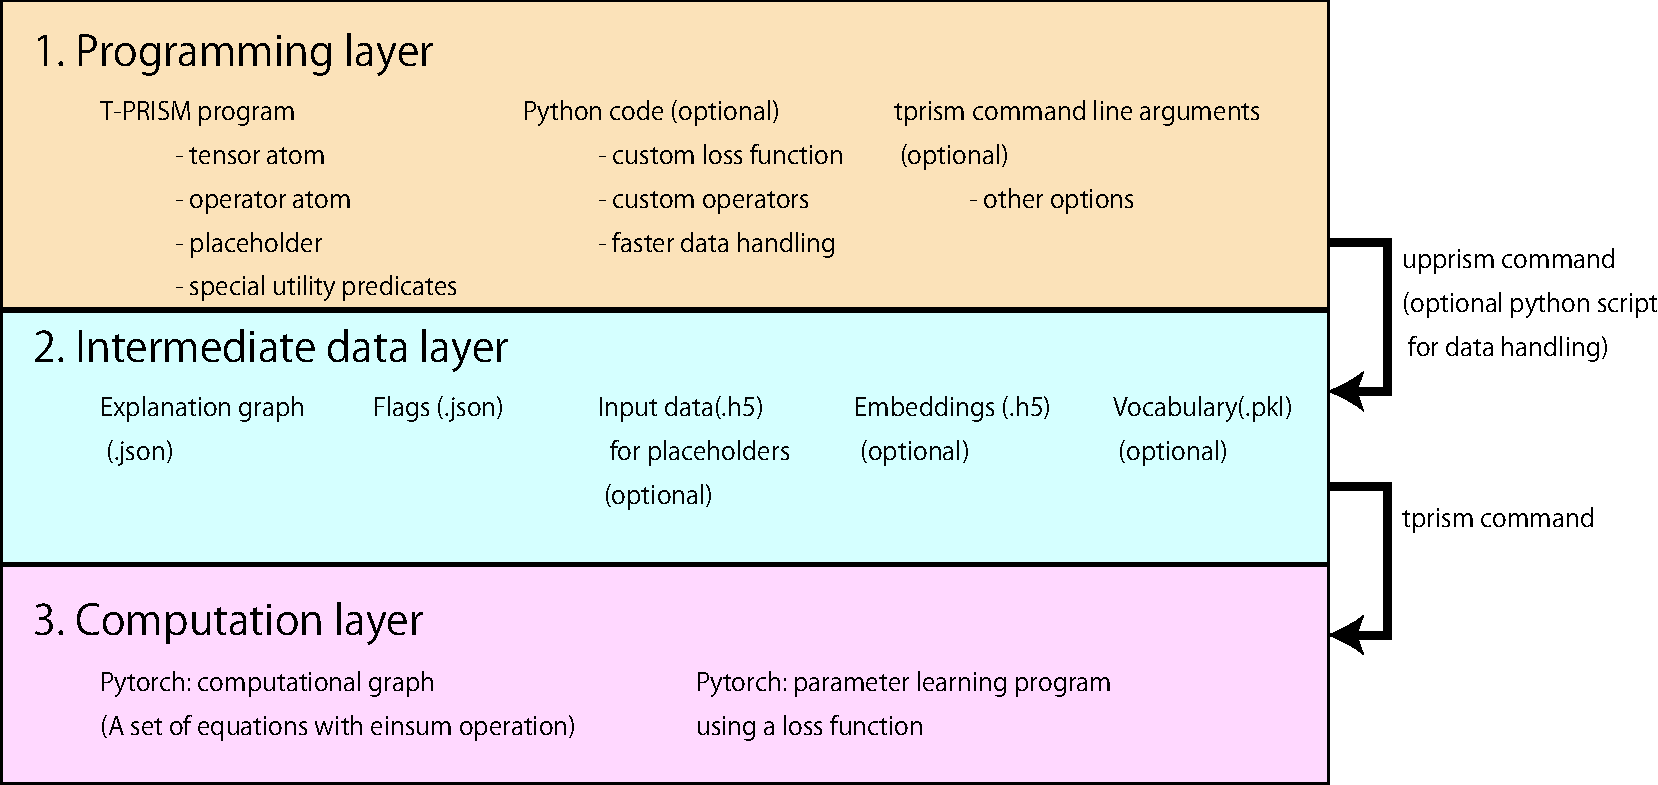
\includegraphics[width=\linewidth]{tprism_system.pdf}
	\caption{Architecture of the T-PRISM system}
	\label{fig:tprismsystem}
\end{figure}

The architecture of the T-PRISM system is shown in
\prettyref{fig:tprismsystem}.  The system consists of three layers: the
{\em programming layer}, where users write programs and settings, the {\em
	intermediate-data layer}, which consists of files, and the {\em computation
	layer}, where PyTorch carries out the tensor computation.  The {\tt upprism}
command connects the programming layer to the intermediate-data layer, and the
{\tt tprism} command (or the Python API) connects the intermediate-data layer
to the computation layer.  This division corresponds to the two parts of the
execution of a T-PRISM program: the symbolic part, i.e., the search for all
proofs of the goals by PRISM, and the numerical part, i.e., the computation of
the tensor equations derived from the proofs.  Since the layers communicate only
through files, each step can be run separately, and the files can be inspected or
produced by other programs such as Python scripts.  Although users directly
operate only the programming layer, they should understand the entire flow.

\subsection*{1. Programming layer}
In the programming layer, users write the following three kinds of inputs.
Only the T-PRISM program is mandatory.
\begin{description}
	\item[T-PRISM program] a PRISM program ({\tt .psm}) defining the model by
	logic.  It contains {\em tensor atoms} declared by {\tt tensor\_atom/2,3} and
	used by {\tt tensor/2}, {\em operator atoms} ({\tt operator/1}) for
	non-linear functions, {\em placeholders} for input data, and calls of the
	{\em special utility predicates}, such as {\tt save\_expl\_graph/3}, which
	export the intermediate data (\prettyref{chap:language} and this chapter).
	Execution flags for training can also be set in the program
	(\prettyref{sec:flags}).
	\item[Python code (optional)] custom loss functions and custom operators,
	which are loaded in the computation layer (\prettyref{chap:loss_op}), and
	scripts for faster data handling, which write tensors and placeholder data
	directly in the intermediate-data layer (\prettyref{chap:intermediate_data}).
	The Python API (\prettyref{chap:python_api}) can be used instead of the {\tt
		tprism} command to control the computation layer from Python programs and
	notebooks.
	\item[{\tt tprism} command-line arguments (optional)] the locations of the
	intermediate files and other options such as training settings
	(\prettyref{chap:tprism_command}).  Options with the same names as execution
	flags override the flags set in the T-PRISM program.
\end{description}

\subsection*{2. Intermediate-data layer}
The intermediate-data layer contains the files listed in
\prettyref{tab:intermediate_files}.  The figure shows their typical formats;
the other available formats are listed in \prettyref{sec:formats} and
\prettyref{chap:intermediate_data}.
\begin{table}[tb]
	\centering
	\small
	\begin{tabular}{P{2.7cm}P{4.6cm}P{6.6cm}}
		\toprule
		File & Created by & Content and use \\
		\midrule
		Explanation graph ({\tt .json}) & {\tt save\_expl\_graph/0-5} & the explanation graph of the goals with tensor atoms and operators, i.e., the structure of the tensor equations \\
		Flags ({\tt .json}) & {\tt save\_expl\_graph/0-5} & the execution flags, and the shapes and types of the tensor atoms \\
		Input data for placeholders ({\tt .h5}, {\tt .json}, {\tt .npy}; optional) & {\tt save\_placeholder\_goals/2-4}, {\tt save\_placeholder\_data/2-4}, or Python & records of values fed to placeholders (option {\tt -{}-dataset}); needed only for programs with placeholders \\
		Embeddings ({\tt .h5}, {\tt .npy}; optional) & {\tt save\_embedding\_\allowbreak from\_pattern/4,5} and its variant, or Python & tensors given to tensor atoms, e.g., input images and fixed matrices (options {\tt -{}-embedding} and {\tt -{}-const\_embedding}) \\
		Vocabulary ({\tt .pkl}; optional) & {\tt tprism} (train and prepare modes) & the correspondence between the values of placeholders and the rows of embedding tables; created automatically and reused in the test mode \\
		\bottomrule
	\end{tabular}
	\caption{Files in the intermediate-data layer}
	\label{tab:intermediate_files}
\end{table}
In addition, the computation layer writes its results, i.e., the model files
with the trained parameters and the output files with the predicted tensors
(\prettyref{sec:tprism_output}).

\subsection*{3. Computation layer}
The computation layer is implemented with PyTorch in the T-PRISM Python package.
\begin{description}
	\item[Computational graph] The explanation graph is converted into a set of
	tensor equations (\prettyref{eq:tprism_eqs}), and each equation is computed
	by {\tt einsum} and the operators, from the tensor atoms at the leaves of the
	explanation graph up to the goals (\prettyref{sec:concepts}).  Tensor atoms
	with placeholders give tensors with a minibatch axis
	(\prettyref{sec:placeholder}), and cyclic explanation graphs are solved by
	fixed-point iteration (\prettyref{sec:cyclic}).
	\item[Parameter learning] A loss function (\prettyref{chap:loss_op}) computes
	the loss of each goal group from the tensors of the goals, the gradients are
	computed by automatic differentiation, and an optimizer updates the
	trainable tensors and the parameters of custom operators
	(\prettyref{sec:training_procedure}).
\end{description}

\subsection*{Commands connecting the layers}
\begin{description}
	\item[{\tt upprism}] runs the T-PRISM program in batch mode: PRISM searches
	for all proofs of the goals by tabled search and constructs the explanation
	graph, and the utility predicates called in {\tt prism\_main/1} save it with
	the other intermediate data.  Python scripts may write tensors and placeholder
	data directly instead (``optional python script for data handling'' in the figure).
	\item[{\tt tprism}] (or the Python API) reads the intermediate files, builds
	the computational graph, and carries out training or prediction.
\end{description}
A standard procedure is executed by the following commands:
\begin{keeptogether}
\begin{shellcode}
$ upprism <T-PRISM program> [arguments ...]
$ tprism train [options ...]
$ tprism test [options ...]
\end{shellcode}
\end{keeptogether}
The search by Prolog is carried out only once by {\tt upprism}.  As long as
the program and the goals are the same, the training can be repeated with
different options without running {\tt upprism} again, and the placeholder data
and embeddings can be replaced by other files of the same structure; for
example, the training data and the test data of {\tt exs/tensor/mlp} share one
explanation graph (\prettyref{sec:nn}).

\subsection*{Example: the quick start in the three layers}
The quick start in \prettyref{sec:quickstart} goes through the layers as follows:
\begin{center}
	\small
	\begin{tabular}{P{3.0cm}P{11.0cm}}
		\toprule
		Layer or command & Quick start \\
		\midrule
		Programming layer & {\tt quickstart.psm}: the tensor atoms {\tt a}, {\tt b}, {\tt r}, the goals
		{\tt goal\_ab} and {\tt goal\_r}, and {\tt prism\_main/1} calling
		{\tt save\_embedding\_from\_pattern/5} and {\tt save\_expl\_graph/3};
		the options {\tt -{}-sgd\_loss rmse\_pair -{}-max\_iterate 1000 \ldots} \\
		{\tt upprism} & {\tt upprism quickstart.psm} \\
		Intermediate-data layer & {\tt quickstart\_tmp/expl.json}, {\tt flags.json}, and the embedding of
		{\tt r} ({\tt r.npy}, {\tt r.npy.json}) \\
		{\tt tprism} & {\tt tprism train \ldots} and {\tt tprism test \ldots} \\
		Computation layer & $(AB)_{ik}=\sum_j A_{ij}B_{jk}$ by {\tt einsum}; the RMSE between $AB$ and $R$;
		the updates of $A$ and $B$ by Adam.  The results are {\tt model.best.model},
		{\tt vocab.pkl} and {\tt quickstart\_out.npy} \\
		\bottomrule
	\end{tabular}
\end{center}

\subsection*{Where to change what}
\begin{center}
	\small
	\begin{tabular}{P{5.2cm}P{8.8cm}}
		\toprule
		Purpose & What to change \\
		\midrule
		change the model (the equations) & the T-PRISM program (\prettyref{chap:language}); run {\tt upprism} again \\
		change the goals & the goals given to {\tt save\_expl\_graph} (\prettyref{sec:save_expl_graph}); run {\tt upprism} again \\
		change the input data & the placeholder data or the embeddings (\prettyref{sec:save_placeholder}, \prettyref{sec:save_embedding}, \prettyref{chap:intermediate_data}) \\
		change the training settings & the options of {\tt tprism} (\prettyref{chap:tprism_command}) or the execution flags (\prettyref{sec:flags}) \\
		add a non-linear function or a neural network layer & a custom operator (\prettyref{sec:custom_op}) \\
		use another loss function & a built-in or custom loss function (\prettyref{chap:loss_op}) \\
		analyze or reuse the results in Python & the Python API (\prettyref{chap:python_api}) \\
		\bottomrule
	\end{tabular}
\end{center}

JSON (extension {\tt .json}) is mainly used for structured data, and
NumPy ({\tt .npy}) and HDF5 ({\tt .h5}) files are used for
multidimensional arrays.  The schema of the structured data is defined by
protocol buffers ({\tt src/c/external/expl.proto}); hence the structured
data can also be saved in the protocol buffers formats, which can be read
from other programming languages.  The formats are described in
\prettyref{chap:intermediate_data}.

\section{Exporting explanation graphs}
\label{sec:save_expl_graph}

The following predicates construct the explanation graph of the goals
and save it, together with the execution flags and the shapes and types of
the tensor atoms:
\begin{description}
	\item[{\tt save\_expl\_graph}]
	saves the explanation graph as {\tt expl.json} and the flags as {\tt
		flags.json}.  The goals are read from the data file specified by the
	flag {\tt data\_source} (by default, the file declared by {\tt data/1}),
	as in {\tt learn/0} of PRISM.
	\item[{\tt save\_expl\_graph({\it Goals})}]
	saves the explanation graph for {\it Goals} as {\tt expl.json} and the flags as {\tt flags.json}.
	\item[{\tt save\_expl\_graph({\it ExplFile},{\it FlagFile})}]
	saves them as {\it ExplFile} and {\it FlagFile}, where the goals are read from the data file.
	\item[{\tt save\_expl\_graph({\it ExplFile},{\it FlagFile},{\it Goals})}]
	saves the explanation graph for {\it Goals} as {\it ExplFile} and the flags as {\it FlagFile}.
	\item[{\tt save\_expl\_graph({\it ExplFile}, {\it FlagFile}, {\it ExplMode}, {\it FlagMode}, {\it Goals})}]
	specifies also the formats: {\tt json} (default), {\tt pb} (protocol
	buffers binary) or {\tt pbtxt} (protocol buffers text).  The formats
	{\tt pb} and {\tt pbtxt} require the build option {\tt USE\_PB=1}.
\end{description}
{\it Goals} is a list of goals or {\em goal groups}, i.e., lists of goals.
A goal that is not in a list forms a goal group by itself.  For example,
{\tt [g1,g2,g3]} gives three goal groups, and {\tt [[g1,g2],[g3,g4]]} gives
two goal groups of pairs.  The explanation graph contains all the goals,
and the goal groups are recorded as the {\em root list}.  Loss functions
are computed for each goal group (\prettyref{sec:goal_group}).  For example,
the following saves the explanation graph for the goals in {\tt sample.dat}:
\begin{prologcode}
prism_main([]) :-
    load_clauses('sample.dat',Gs),
    save_expl_graph('sample_tmp/expl.json','sample_tmp/flags.json',Gs).
\end{prologcode}
The directory of the output files must exist.  While saving, {\tt upprism}
prints messages such as {\tt \#goals: 0(2)} (the progress of the search and the
number of goals in parentheses) and {\tt [SAVE:json]} followed by the name of
each saved file.  If PRISM cannot find any proof of a goal, the execution stops
with an error (\prettyref{sec:troubleshooting}).

\subsection*{Saving only the flags}
The following predicates save the current values of the execution flags
as {\it FlagFile} (default: {\tt flags.json}) in the format {\it FlagMode}
(default: {\tt json}):
\begin{itemize}
	\item {\tt save\_flags}
	\item {\tt save\_flags({\it FlagFile})}
	\item {\tt save\_flags({\it FlagFile},{\it FlagMode})}
\end{itemize}
Note that the flag files written by these predicates do not contain the
shapes of the tensor atoms, which {\tt tprism} requires; use the flag file
written by {\tt save\_expl\_graph}.

\section{Exporting placeholder data}
\label{sec:save_placeholder}

The following predicates construct placeholders and records of their
values from goals (\prettyref{sec:placeholder}) and save the records as
{\it Filename} in the format {\it Mode}:
\begin{itemize}
	\item {\tt save\_placeholder\_goals({\it PlaceholderGoals},{\it Goals})}
	\item {\tt save\_placeholder\_goals({\it Filename},{\it PlaceholderGoals},{\it Goals})}
	\item {\tt save\_placeholder\_goals({\it Filename},{\it Mode},{\it PlaceholderGoals},{\it Goals})}
\end{itemize}
{\it Mode} is one of {\tt npy}, {\tt json}, {\tt hdf5}, {\tt pb} and {\tt pbtxt}.
The default file name and format are {\tt data.h5} and {\tt hdf5}, which
require the build option {\tt USE\_H5=1}; with the pre-built packages, use
{\tt npy} or {\tt json}.

{\it PlaceholderGoals} is a list of patterns, i.e., goals (or goal groups)
containing variables, and {\it Goals} is a list of ground goals (or goal
groups).  For each pattern, the elements of {\it Goals} matching the
pattern are collected, and the values of the variables in each matched
element form a record.  The records of the $n$-th pattern are saved as the
$n$-th goal (with the goal ID $n-1$) in the file.  Finally, the variables
in {\it PlaceholderGoals} are bound to the placeholder atoms {\tt
	'\$placeholder1\$'}, {\tt '\$placeholder2\$'}, \ldots in the order of
appearance, so that the explanation graph can be constructed for the
patterns.  For example:
\begin{prologcode}
prism_main([]) :-
    Goals=[pred(1),pred(2),pred(3),pred(5),pred(8)],
    PlaceholderGoals=[pred(_)],
    save_placeholder_goals('data',npy,PlaceholderGoals,Goals).
\end{prologcode}
Here, {\tt PlaceholderGoals} becomes {\tt [pred('\$placeholder1\$')]}, and
the records $(1), (2), (3), (5), (8)$ are saved for {\tt \$placeholder1\$}.
For a more complex example with two predicates:
\begin{prologcode}
prism_main([]) :-
    Goals=[pred1(1,4),pred1(2,3),pred1(3,2),pred2(5,1),pred2(8,0)],
    PlaceholderGoals=[pred1(_,_),pred2(_,_)],
    save_placeholder_goals('data',npy,PlaceholderGoals,Goals),
    save_expl_graph('expl.json','flags.json',PlaceholderGoals).
\end{prologcode}
{\tt PlaceholderGoals} becomes
\begin{prologcode}
[pred1('$placeholder1$','$placeholder2$'),pred2('$placeholder3$','$placeholder4$')]
\end{prologcode}
and the following records are saved:
\begin{center}
	\begin{tabular}{llll}
		\toprule
		goal ID & pattern & placeholders & records \\
		\midrule
		0 & {\tt pred1(\_,\_)} & {\tt \$placeholder1\$}, {\tt \$placeholder2\$} & $(1,4),(2,3),(3,2)$ \\
		1 & {\tt pred2(\_,\_)} & {\tt \$placeholder3\$}, {\tt \$placeholder4\$} & $(5,1),(8,0)$ \\
		\bottomrule
	\end{tabular}
\end{center}
The output files depend on the format:
\begin{description}
	\item[{\tt npy}] {\it Filename} is a directory, which is created if necessary.
	The records of the goal $k$ are saved as an integer matrix (the number of records
	$\times$ the number of placeholders) in {\it Filename}{\tt /placeholder\_}$k${\tt .npy},
	and the list of the files and placeholders is saved in {\it Filename}{\tt /placeholder.npy.json}.
	Give the latter to {\tt tprism}.
	\item[{\tt json}, {\tt pb}, {\tt pbtxt}] The records are saved in a file whose name is
	{\it Filename} followed by a suffix {\tt $n$\_$m$} (e.g., {\tt data.json1\_0} for
	{\it Filename} {\tt data.json} and one pattern), and a large number of records is
	split into several files.  Use the extension {\tt .json} for {\it Filename} in
	the {\tt json} format so that {\tt tprism} recognizes the files.
	\item[{\tt hdf5}] The records are saved in an HDF5 file {\it Filename}
	with a group for each goal (\prettyref{sec:placeholder_file}).
\end{description}

\subsection*{Low-level predicates}
The following predicates directly save a list of placeholders and their records without pattern matching:
\begin{itemize}
	\item {\tt save\_placeholder\_data({\it Placeholders},{\it Data})}
	\item {\tt save\_placeholder\_data({\it Filename},{\it Placeholders},{\it Data})}
	\item {\tt save\_placeholder\_data({\it Filename},{\it Mode},{\it Placeholders},{\it Data})}
\end{itemize}
{\it Placeholders} is a list (one element for each goal) of lists of
placeholder atoms, and {\it Data} is a list (one element for each goal) of
lists of records, each of which is a list of values.  For example, the two
examples above correspond to the following arguments, respectively:
\begin{prologcode}
Placeholders=[['$placeholder1$']],
Data=[[[1],[2],[3],[5],[8]]]

Placeholders=[['$placeholder1$','$placeholder2$'],['$placeholder3$','$placeholder4$']],
Data=[[[1,4],[2,3],[3,2]],[[5,1],[8,0]]]
\end{prologcode}

\section{Exporting tensors}
\label{sec:save_embedding}

The following predicates construct a tensor from the solutions of a goal
and save it as an embedding file, which gives the tensor to a tensor atom:
\begin{itemize}
	\item {\tt save\_embedding\_from\_pattern({\it Vars},{\it Pattern},{\it Target},{\it FileNameBase})}
	\item {\tt save\_embedding\_from\_pattern({\it Vars},{\it Pattern},{\it Target},{\it FileNameBase},{\it Mode})}
	\item {\tt save\_embedding\_from\_pattern\_with\_value({\it Vars},{\it Val},{\it Pattern},{\it Target},{\it FileNameBase})}
	\item {\tt save\_embedding\_from\_pattern\_with\_value({\it Vars},{\it Val},{\it Pattern},{\it Target},{\it FileNameBase},{\it Mode})}
\end{itemize}
{\tt save\_embedding\_from\_pattern} collects the instances of the list of
variables {\it Vars} for which the goal {\it Pattern} succeeds (as {\tt
	findall/3}), and constructs a tensor whose axes correspond to the
elements of {\it Vars}: for each axis, the distinct values of the
corresponding variable are sorted in the standard order of terms and
numbered from 0.  The element at the position of each instance is set to
one, and the other elements are zero.  {\tt
	save\_embedding\_from\_pattern\_with\_value} sets the element to the value
of {\it Val} instead of one.  {\it Target} is a term {\tt tensor({\it
		Name})}, which specifies the tensor atom {\it Name} to which the tensor is
given.  {\it Mode} is {\tt hdf5} (default) or {\tt npy}.

For example, given the facts
\begin{prologcode}
rel1(a,a). rel1(b,b). rel1(c,c).
rel1(a,b). rel1(b,c). rel1(c,a).
\end{prologcode}
{\tt save\_embedding\_from\_pattern([X,Y],rel1(X,Y),tensor(rel1),'tmp/embedding',npy)}
constructs a $3\times 3$ binary matrix (the adjacency matrix of the
relation) whose $(x,y)$ element is one if and only if {\tt rel1($x$,$y$)}
holds, and associates it with the tensor atom {\tt rel1}.  The relation
does not have to be given by facts; any goal, e.g., a rule computing a
relation, can be used as {\it Pattern} (\prettyref{sec:tutorial_construction}).
Note that the shape of the tensor is the number of distinct values for each
axis, which must agree with the declaration by {\tt tensor\_atom/2}.  The
lists of the values are displayed, e.g., {\tt [[a,b,c],[a,b,c]]}.

The output files are as follows:
\begin{description}
	\item[{\tt npy}] the tensor is saved in {\it FileNameBase}{\tt .npy}, and
	its metadata (the file name, the group {\tt train}, the dataset name and
	the shape) in {\it FileNameBase}{\tt .npy.json}.  Give the latter to {\tt tprism}.
	\item[{\tt hdf5}] the tensor is saved in the group {\tt train} of {\it
		FileNameBase}{\tt .h5}.  This format supports only vectors and matrices
	and requires the build option {\tt USE\_H5=1}.
\end{description}
In both formats, the table of the values for each axis is saved in {\it
	FileNameBase}{\tt .txt}, a tab-separated file with the columns {\tt axis},
{\tt index} and {\tt label}.  The dataset name of the tensor is derived from
{\it Target}, e.g., {\tt tensor\_rel1\_} (\prettyref{sec:tensor_name}).

\section{File formats and build options}
\label{sec:formats}

The formats supported by the built-in predicates depend on the build options of PRISM (\prettyref{sec:install_prism}):
\begin{center}
	\begin{tabular}{P{6.4cm}llll}
		\toprule
		Predicates & {\tt json} & {\tt npy} & {\tt hdf5} & {\tt pb}, {\tt pbtxt} \\
		\midrule
		{\tt save\_expl\_graph/0-5} & default & -- & -- & {\tt USE\_PB} \\
		{\tt save\_flags/0-2} & default & -- & -- & {\tt USE\_PB} \\
		{\tt save\_placeholder\_goals/2-4}, \newline {\tt save\_placeholder\_data/2-4} & yes & {\tt USE\_NPY} & default ({\tt USE\_H5}) & {\tt USE\_PB} \\
		{\tt save\_embedding\_from\_pattern/4,5}, \newline {\tt save\_embedding\_from\_pattern\_\allowbreak with\_value/5,6} & -- & {\tt USE\_NPY} & default ({\tt USE\_H5}) & -- \\
		\bottomrule
	\end{tabular}
\end{center}
The pre-built packages are built with {\tt USE\_NPY=1}; hence, specify
{\tt npy} (or {\tt json} for placeholder data) explicitly.  When a format
is not available, an error message such as ``{\tt [ERROR] hdf5 format is
	not implemented (please compile prism with the USE\_H5 option)}'' is
displayed.  Note that the {\tt tprism} command reads HDF5 files by h5py, so
HDF5 files created by Python scripts can be used regardless of the build
options.

\section{Execution flags}
\label{sec:flags}

The training and computation in {\tt tprism} are controlled by execution
flags of PRISM.  They are set in a program by {\tt set\_prism\_flag/2}, e.g.,
\begin{prologcode}
:- set_prism_flag(sgd_learning_rate,0.01).
prism_main([]) :-
    set_prism_flag(max_iterate,100),
    set_prism_flag(sgd_loss,ce_pl('$placeholder2$')),
    ...
    save_expl_graph('tmp/expl.json','tmp/flags.json',Goals).
\end{prologcode}
and the values at the time of {\tt save\_expl\_graph} are exported to the
flag file.  The same settings can be given to {\tt tprism} as
command-line options with the same names (e.g., {\tt -{}-sgd\_learning\_rate
	0.01}).  The values are merged in the following order (weakest first): the
defaults of {\tt tprism}, the values in the flag file, and the
command-line options.  The flags related to T-PRISM are listed below:
\begin{center}
	\small
	\begin{tabular}{lll}
		\toprule
		Flag & Default & Description \\
		\midrule
		{\tt sgd\_minibatch\_size} & 1 & the number of records in a minibatch (with placeholder data) \\
		{\tt max\_iterate} & 10 & the maximum number of epochs (iterations for cyclic programs) \\
		{\tt sgd\_learning\_rate} & 0.0001 & the learning rate \\
		{\tt sgd\_loss} & {\tt base\_loss} & the loss function (\prettyref{sec:specify_loss}) \\
		{\tt sgd\_optimizer} & {\tt adam} & the optimizer: {\tt adam}, {\tt adadelta} or {\tt sgd} \\
		{\tt sgd\_weight\_decay} & 0.01 & the weight decay (the coefficient of the $L_2$ penalty) \\
		{\tt sgd\_adam\_beta} & 0.9 & $\beta_1$ of Adam \\
		{\tt sgd\_adam\_gamma} & 0.999 & $\beta_2$ of Adam \\
		{\tt sgd\_adam\_epsilon} & $10^{-8}$ & $\epsilon$ of Adam \\
		{\tt sgd\_adadelta\_gamma} & 0.95 & $\rho$ of AdaDelta \\
		{\tt sgd\_adadelta\_epsilon} & $10^{-8}$ & $\epsilon$ of AdaDelta \\
		{\tt sgd\_patience} & 3 & early stopping: epochs allowed without improvement \\
		{\tt sgd\_valid\_ratio} & 0.1 & the ratio of validation records (0 disables validation) \\
		{\tt sgd\_goal\_valid\_ratio} & 0.0 & the ratio of validation goals (0 disables it) \\
		\bottomrule
	\end{tabular}
\end{center}
Note the following points:
\begin{itemize}
	\item The defaults of {\tt sgd\_learning\_rate}, {\tt sgd\_weight\_decay}
	and {\tt sgd\_optimizer} are those of PRISM, which are always exported to
	the flag file.  The other flags are exported as {\tt default} (unset)
	unless they are set in the program, and then the defaults of {\tt tprism} apply.
	\item {\tt max\_iterate} accepts {\tt inf}.  The option {\tt -{}-epoch} of {\tt tprism} is an alias of {\tt -{}-max\_iterate}.
	\item {\tt sgd\_penalty} is the old name of {\tt sgd\_weight\_decay} and is still accepted.
	\item Some of the flags are also used by the learning procedures of PRISM; see the PRISM User's Manual.
	\item A placeholder in a loss function must be quoted in programs, as
	{\tt ce\_pl('\$placeholder2\$')} above, because B-Prolog does not accept
	{\tt \$placeholder2\$} unquoted.  A float in a compound term,
	e.g., {\tt ce(0.1)}, is exported with six digits after the decimal point.
	\item The PRISM flag {\tt error\_on\_cycle} must be {\tt off} for cyclic programs (\prettyref{sec:cyclic}).
\end{itemize}

%%%%%%%%%%%%%%%%%%%%%%%%%%%%%%%%%%%%%%%%%%%%%%%%%%%%%%%%%%%%%%%%%%%%%%%%%%%
\chapter{The {\tt tprism} command}
\label{chap:tprism_command}

The {\tt tprism} command reads the files in the intermediate-data layer
and carries out training and prediction.  It is executed in the following format:
\begin{keeptogether}
\begin{shellcode}
$ tprism <mode> [options ...]
\end{shellcode}
\end{keeptogether}

\section{Modes}
\label{sec:tprism_mode}

\begin{description}
	\item[{\tt train}]
	builds the computational explanation graph and trains the parameters.
	Without placeholder data, all goals are evaluated at once in each epoch
	(full-batch training).  With placeholder data ({\tt -{}-dataset}), the
	parameters are trained by minibatches with validation and early stopping
	(\prettyref{sec:training_procedure}); after the training, the goals are
	evaluated on the training data, and the test loss is displayed.  With the
	option {\tt -{}-cycle}, the fixed point of the tensor equations of a cyclic
	program is computed instead of training (\prettyref{sec:cyclic}).  The
	vocabulary file and, except with {\tt -{}-cycle}, the model files are created.
	\item[{\tt test} (or {\tt pred})]
	loads the vocabulary file and the trained parameters ({\it
		model}{\tt .best.model} if it exists), evaluates the goals, and saves the
	outputs (\prettyref{sec:tprism_output}).  The loss is displayed if a loss
	function is given.  With the option {\tt -{}-cycle}, the fixed point of the
	tensor equations of a cyclic program is computed and saved as the output
	(\prettyref{sec:cyclic}).  With placeholder data, the vocabulary file
	created in the training phase is required (the {\tt prepare} mode creates
	it without training); without placeholder data, the vocabulary file is
	created if it does not exist.
	\item[{\tt prepare}]
	creates only the vocabulary file.
\end{description}

\section{Input files}
\label{sec:tprism_input}

\begin{description}
	\item[{\tt -{}-input} {\it INPUT}, {\tt -I} {\it INPUT}]
	specifies the location of the intermediate files.  If {\it INPUT} is an
	existing directory (e.g., {\tt -{}-input tmp} or {\tt -{}-input tmp/}),
	the default file names in it are used.  Otherwise, {\it INPUT} is
	regarded as a prefix of the file names, and a dot is inserted:
	\begin{center}
		\begin{tabular}{lll}
			\toprule
			File & {\tt -{}-input dir/} & {\tt -{}-input dir/name} \\
			\midrule
			explanation graph & {\tt dir/expl.json} & {\tt dir/name.expl.json} \\
			flags & {\tt dir/flags.json} & {\tt dir/name.flags.json} \\
			model & {\tt dir/model} & {\tt dir/name.model} \\
			vocabulary & {\tt dir/vocab.pkl} & {\tt dir/name.vocab.pkl} \\
			\bottomrule
		\end{tabular}
	\end{center}
	The model name is a base name: the files {\it model}{\tt .best.model}
	and {\it model}{\tt .last.model} are written in training.
	\item[{\tt -{}-expl\_graph} {\it FILE}, {\tt -{}-flags} {\it FILE}, {\tt -{}-model} {\it FILE}, {\tt -{}-vocab} {\it FILE}]
	specify the explanation graph, the flag file, the model name and the
	vocabulary file individually, overriding {\tt -{}-input}.
	\item[{\tt -{}-dataset} {\it FILE} \ldots]
	specifies the placeholder data: HDF5 files ({\tt .h5}), JSON files
	({\tt .json} and the files with a suffix such as {\tt .json1\_0}), or
	{\tt .npy.json} files (\prettyref{sec:placeholder_file}).  Multiple files
	are merged: the records of the same goal ID are concatenated.
	\item[{\tt -{}-embedding} {\it FILE} \ldots]
	specifies embedding files ({\tt .h5} or {\tt .npy.json}) giving
	tensors to tensor atoms (\prettyref{sec:embedding_file}).  The group of
	the files is selected by the mode: {\tt train} in the train mode and {\tt
		test} in the test mode.  For tensor atoms with placeholders, the values of
	the placeholders select the rows of the arrays (\prettyref{sec:placeholder}).
	\item[{\tt -{}-const\_embedding} {\it FILE} \ldots]
	specifies constant embedding files, which are the same as {\tt
		-{}-embedding} except that the group {\tt train} is always used
	regardless of the mode.  Use this option for fixed tensors that do not
	depend on the phase, such as adjacency matrices.  Since the files created by {\tt
		save\_embedding\_from\_pattern} have only the group {\tt train}, give
	them by this option to use them in the test mode.
	\item[{\tt -{}-intermediate\_data\_prefix} {\it PREFIX}, {\tt -{}-data} {\it FILE} \ldots]
	are deprecated aliases.  The former sets the files {\it PREFIX}{\tt
		expl.json}, {\it PREFIX}{\tt flags.json}, {\it PREFIX}{\tt model} and
	{\it PREFIX}{\tt vocab.pkl} (without inserting a separator), and the
	latter is equivalent to {\tt -{}-dataset}.
\end{description}

\section{Training options}
\label{sec:tprism_training_option}

The following options correspond to the execution flags with the same
names (\prettyref{sec:flags}) and override the values in the flag file:
\begin{keeptogether}
\begin{shellcode}
--sgd_minibatch_size N     --max_iterate N (--epoch N)   --sgd_learning_rate R
--sgd_loss TERM            --sgd_optimizer NAME          --sgd_weight_decay R
--sgd_adam_beta R          --sgd_adam_gamma R            --sgd_adam_epsilon R
--sgd_adadelta_gamma R     --sgd_adadelta_epsilon R      --sgd_patience N
--sgd_valid_ratio R        --sgd_goal_valid_ratio R
\end{shellcode}
\end{keeptogether}
A loss function with arguments must be quoted so that the shell does not
expand {\tt \$}, e.g., {\tt -{}-sgd\_loss 'ce\_pl(\$placeholder2\$)'}.  In
addition, {\tt -{}-cycle} enables the computation of cyclic explanation graphs (\prettyref{sec:cyclic}).

\section{Other options}
\begin{description}
	\item[{\tt -{}-output} {\it FILE}]
	the file for the outputs in the test mode, saved by {\tt numpy.save}
	(the extension {\tt .npy} is appended if it is missing).  The default is
	{\tt ./output.pkl}, i.e., {\tt ./output.pkl.npy} is created.
	\item[{\tt -{}-config} {\it FILE}]
	a JSON file of option values whose keys are the option names without
	{\tt -{}-}, e.g.,
\begin{keeptogether}
\begin{shellcode}
{"max_iterate": 100, "sgd_learning_rate": 0.01}
\end{shellcode}
\end{keeptogether}
	The values in the file override the command-line options.
	\item[{\tt -{}-cpu}, {\tt -{}-gpu} {\it IDS}]
	set the environment variable {\tt CUDA\_VISIBLE\_DEVICES}: {\tt -{}-cpu}
	hides all GPUs, and {\tt -{}-gpu 0,2} makes the GPUs 0 and 2 visible.
	Note that the current version of {\tt tprism} carries out the computation on the CPU.
	\item[{\tt -{}-verbose}, {\tt -v}] shows all debug messages.
	\item[{\tt -{}-debug\_verb} {\it CATEGORY} \ldots]
	shows only the debug messages of the given categories: {\tt feed}
	(feeding data to placeholders and minibatches), {\tt module} (loading
	plugins and operator modules), {\tt minibatch} (processing of
	minibatches), {\tt embedding} (assigning tensors to switches), {\tt graph}
	(construction of the computational graph), and {\tt param} (shapes of
	parameters).
	\item[{\tt -{}-no\_verb}] shows only warnings and errors.
\end{description}

\section{Training procedure}
\label{sec:training_procedure}

\subsection*{Training without placeholder data}
In each epoch, all goals are evaluated, and the parameters are updated
once with the mean of the losses of the goal groups, to which
regularization terms such as those of {\tt sparse} tensors are added.  If
{\tt sgd\_goal\_valid\_ratio} is positive, this ratio of the goal groups is
chosen randomly and held out for validation: these goal groups are
evaluated in each epoch but not used for updating the parameters, and early
stopping is applied to their loss.  The parameters with the smallest
training loss (or validation loss if validation goals exist) are saved as
{\it model}{\tt .best.model}, and the final parameters as {\it model}{\tt .last.model}.

\subsection*{Training with placeholder data}
For each goal (pattern) of the placeholder data, the records are shuffled
and the ratio {\tt sgd\_valid\_ratio} of them is held out as validation
records.  The training records are divided into minibatches of size {\tt
	sgd\_minibatch\_size}; the records exceeding a multiple of the minibatch
size are left out in each epoch (since the records are shuffled in every
epoch, they are used in other epochs).  The validation loss is computed
after each epoch, and early stopping is enabled only when at least one full
minibatch of validation records exists.  If {\tt sgd\_goal\_valid\_ratio}
is positive, whole goals are also held out as validation goals.

\subsection*{Early stopping and logs}
Training stops when the validation loss has not improved for {\tt
	sgd\_patience} epochs.  The parameters with the best validation loss are
saved as {\it model}{\tt .best.model}, and the final parameters as {\it
	model}{\tt .last.model}.  A line of the training log looks as follows:
\begin{keeptogether}
\begin{shellcode}[basicstyle=\ttfamily\footnotesize]
[   1]  train-loss: 2.277  *train-accuracy: 0.201 valid-loss: 2.226  *valid-accuracy: 0.330 ( 0) *
\end{shellcode}
\end{keeptogether}
The number in parentheses is the number of epochs without improvement,
and the last {\tt *} indicates that the validation loss improved.
The metrics marked with {\tt *}, such as the accuracy, are computed by the
loss function for information and are not included in the loss
(\prettyref{sec:custom_loss}).

\section{Output files}
\label{sec:tprism_output}

\begin{itemize}
	\item The vocabulary file ({\tt -{}-vocab}) is created in the train and prepare modes and read in the test mode.
	\item The model files {\it model}{\tt .best.model} and {\it model}{\tt
		.last.model} contain the parameters as a state dictionary of PyTorch
	(\prettyref{sec:model_file}).
	\item In the test mode, the outputs are saved in {\tt -{}-output}.  The
	structure of the array depends on the loss function
	(\prettyref{sec:builtin_loss}): e.g., with {\tt rmse\_pair}, the shape is
	(the number of goal groups, 2, \ldots), and with the default {\tt
		base\_loss}, (the number of goals, \ldots).  With placeholder data, the
	outputs of the minibatches are concatenated for each goal (pattern).
	In addition, a pickle file {\tt output.pkl} is written in the current
	directory, which contains a dictionary from the IDs of the root goals to
	dictionaries with the keys {\tt name} (the predicate name) and {\tt
		data} (the output).
\end{itemize}

\section{Examples}
The Markov chain program (\prettyref{sec:markov_chain}) is trained with
the negative log likelihood loss as follows:
\begin{keeptogether}
\begin{shellcode}
$ upprism markov_chain.psm
$ tprism train --input ./markov_chain_tmp/ --sgd_loss nll \
      --max_iterate 10 --sgd_learning_rate 0.01 --cpu
\end{shellcode}
\end{keeptogether}
A multi-layer perceptron with placeholder data and an embedding file of
images (\prettyref{sec:nn}; the placeholder data in the HDF5 format require
PRISM built with {\tt USE\_H5=1}) is trained and tested as follows:
\begin{keeptogether}
\begin{shellcode}
$ tprism train --input ./mnist_tmp/mnist --dataset ./mnist_tmp/mnist_data.train.h5 \
      --embedding ./mnist/mnist.h5 --sgd_loss 'ce_pl($placeholder2$)' \
      --max_iterate 10 --sgd_minibatch_size 1000 --sgd_learning_rate 0.001
$ tprism test --input ./mnist_tmp/mnist --dataset ./mnist_tmp/mnist_data.test.h5 \
      --embedding ./mnist/mnist.h5 --sgd_loss 'ce_pl($placeholder2$)' \
      --output mnist_output.npy
\end{shellcode}
\end{keeptogether}

\section{Troubleshooting}
\label{sec:troubleshooting}

The following messages are often displayed by {\tt upprism} and {\tt tprism}:
\begin{description}
	\item[{\tt PRISM ERROR: outcome space not given -{}- tensor(b)}]
	({\tt upprism}) the tensor atom {\tt b} is used in a clause body but not
	declared by {\tt tensor\_atom/2,3} (\prettyref{sec:tensor_atom}).
	\item[{\tt PRISM ERROR: no explanations -{}- g}]
	({\tt upprism}) the goal {\tt g} has no proofs.  Check that the goal
	succeeds as a Prolog goal and that all index symbols in the tensor atoms are
	collected or declared by {\tt index\_atoms/1} (\prettyref{sec:index}); a
	tensor atom with an unknown index symbol fails.
	\item[{\tt Aborted by exception -{}- error(prism\_runtime\_error(cycle\_detected),...)}]
	({\tt upprism}) the explanation graph is cyclic; set the flag {\tt
		error\_on\_cycle} to {\tt off} (\prettyref{sec:cyclic}).
	\item[{\tt [ERROR] hdf5 format is not implemented (please compile prism with the USE\_H5 option)}]
	({\tt upprism}) the format is not available in the build of PRISM; use
	{\tt npy} or {\tt json}, or build PRISM with {\tt USE\_H5=1} (\prettyref{sec:formats}).
	\item[{\tt missmatch indices: [...]}]
	({\tt tprism}, warning) the clauses of a goal give tensors with different
	free indices; their tensors are added by the positions of the axes
	(\prettyref{sec:einsum}).
	\item[{\tt AssertionError: index symbol mismatch:'j':4!=3}]
	({\tt tprism}) the index symbol {\tt j} is used for axes of different sizes
	in a clause body.
	\item[{\tt AssertionError: foo is not found}]
	({\tt tprism}) the operator {\tt foo} is unknown; register a custom operator
	(\prettyref{sec:custom_op}).
	\item[{\tt unknown loss function: foo (available: ...)}]
	({\tt tprism}, warning) the loss function is unknown, and no loss function is
	used.  Then training stops with the error {\tt loss is None} or {\tt
		output/loss is None in training} (\prettyref{sec:specify_loss}).
	\item[{\tt no conversion from values to indices: \$placeholder2\$ ...}]
	({\tt tprism}, warning) the placeholder does not occur in any tensor atom,
	e.g., a label for {\tt ce\_pl}; this is harmless (\prettyref{sec:placeholder}).
	\item[{\tt [SKIP] skip loading: ... is not found}]
	({\tt tprism}, warning) the model file of the test mode does not exist, and
	the parameters are not trained ones; check {\tt -{}-model} and {\tt -{}-input}.
	\item[{\tt FileNotFoundError: ... vocab.pkl}]
	({\tt tprism test}) with placeholder data, the vocabulary file created in
	training is required; run the train or prepare mode with the same {\tt -{}-vocab}.
	\item[{\tt Missing key(s) in state\_dict: "tensor\_r\_"}]
	({\tt tprism test}) the tensor {\tt r} was given by an embedding file in
	training but not in the test mode, so it became a trainable parameter.  A
	file with only the group {\tt train} (e.g., created by {\tt
		save\_embedding\_from\_pattern}) must be given by {\tt -{}-const\_embedding}
	to be used in the test mode (\prettyref{sec:tprism_input}).
	\item[{\tt FileNotFoundError} for an {\tt .npy} file]
	the file names in {\tt .npy.json} files are relative to the directory where
	they were saved; run {\tt tprism} in that directory (\prettyref{chap:intermediate_data}).
	\item[{\tt [geotorch] disabled}]
	({\tt tprism}, warning) geotorch is not installed; this is harmless unless
	constrained tensors are used (\prettyref{sec:tensor_type}).
\end{description}
For details, the options {\tt -{}-verbose} and {\tt -{}-debug\_verb} show debug
messages, and {\tt probf/1} of PRISM displays the explanation graph of a goal
(\prettyref{sec:program_structure}).

%%%%%%%%%%%%%%%%%%%%%%%%%%%%%%%%%%%%%%%%%%%%%%%%%%%%%%%%%%%%%%%%%%%%%%%%%%%
\chapter{Loss functions and operators}
\label{chap:loss_op}

Loss functions and operators are implemented as Python classes, i.e.,
{\em plugins}.  The {\tt tprism} package provides standard ones, and users
can add their own.

\section{Specifying a loss function}
\label{sec:specify_loss}

A loss function is specified by the flag {\tt sgd\_loss}, the option {\tt
	-{}-sgd\_loss} of {\tt tprism}, or the argument {\tt loss\_cls} or {\tt
	loss\_obj} of {\tt TprismModel} in the Python API.  The value of the flag
and the option is a Prolog term: a name of a loss function such as {\tt
	ce}, or a name with arguments such as {\tt preference\_pair(0.5)} and {\tt
	ce\_pl(\$placeholder2\$)}.  The arguments are passed to the loss function
as strings; quoted atoms are unquoted.  On the command line, quote the term
so that the shell does not expand {\tt \$}; in a program, quote the
placeholder atom:
\begin{keeptogether}
\begin{shellcode}
$ tprism train ... --sgd_loss 'ce_pl($placeholder2$)'
:- set_prism_flag(sgd_loss,ce_pl('$placeholder2$')).
\end{shellcode}
\end{keeptogether}
The name of a loss function is the name of its class converted into snake
case, e.g., {\tt PreferencePair} $\rightarrow$ {\tt preference\_pair} and
{\tt RMSEPair} $\rightarrow$ {\tt rmse\_pair}.  An unknown name is reported
as the warning ``{\tt unknown loss function}'', and no loss function is used;
then training fails, whereas prediction still works.

\section{Goal groups and loss functions}
\label{sec:goal_group}

A loss function receives the values of all goals and computes a loss for
each goal group (\prettyref{sec:save_expl_graph}).  A goal that is not in a
list forms a goal group by itself.  Loss functions comparing two goals,
such as {\tt preference\_pair} and {\tt rmse\_pair}, use the first and the
second goals of each group.  For example:
\begin{itemize}
	\item {\tt save\_expl\_graph(E,F,[[goal\_ab,goal\_r]])} gives one goal
	group for {\tt rmse\_pair}, comparing $AB$ with $R$ (\prettyref{sec:quickstart}).
	\item In DistMult (\prettyref{sec:distmult01}), the goals are pairs {\tt
		[rel($s$,$o$,$r$),rel($s$,$o'$,$r$)]} of a positive and a negative example for {\tt preference\_pair}.
	\item In classification, e.g., {\tt [output(5,0),output(0,1),\ldots]}, each goal forms a goal group for {\tt ce}.
\end{itemize}
In training without placeholder data, the loss is the mean of the losses
of the goal groups.  With placeholder data, the $k$-th pattern of the
placeholder data corresponds to the $k$-th goal group of the explanation
graph, and its loss is computed for each minibatch.

\section{Built-in loss functions}
\label{sec:builtin_loss}

\prettyref{tab:losses} summarizes the built-in loss functions, and the details are given below.
\begin{table}[tb]
	\centering
	\small
	\begin{tabular}{lP{4.4cm}P{3.0cm}P{3.4cm}}
		\toprule
		Name & Goal group & Label & Typical use \\
		\midrule
		{\tt base\_loss} & any & -- & prediction only (no training) \\
		{\tt nll} & goals whose values are probabilities & -- & PRISM-like models \\
		{\tt ce} & a single goal with a vector of class scores & the first argument of the goal & classification without placeholders \\
		{\tt ce\_pl($P$)} & a single goal with a minibatch of class scores & the values of the placeholder $P$ & classification with placeholders \\
		{\tt preference\_pair($\gamma$)} & a pair of a positive and a negative goal & the order in the pair & ranking, knowledge graph embedding \\
		{\tt rmse\_pair} & a pair of goals with tensors of the same shape & the second goal & fitting a tensor \\
		{\tt mse} & a pair of goals with tensors of the same shape & the second goal & fitting a tensor \\
		\bottomrule
	\end{tabular}
	\caption{Built-in loss functions}
	\label{tab:losses}
\end{table}

\begin{description}
	\item[{\tt base\_loss}] (the default) no loss function.  The output is
	the tensors of all goals stacked (the number of goals $\times$ \ldots).
	Training is not possible; this is used to compute tensors, e.g., in the
	test mode and for cyclic programs.
	\item[{\tt nll}] the negative log likelihood $-\log q(G)$ of a goal $G$
	whose value $q(G)$ is a probability, averaged over the goals of each
	goal group.  It is used for PRISM-like models (\prettyref{sec:markov_chain}, \prettyref{sec:simulated_msw}).
	\item[{\tt ce}] the cross-entropy loss for classification.  The first
	argument of each goal is its correct label, a class number starting from
	0, and the tensor of the goal is a vector of unnormalized scores (logits)
	of the classes; the softmax function is applied in the loss function.
	For example, the goal {\tt output(5,0)} represents that the image 0 has
	the label 5 (\prettyref{sec:mlp0}).  The accuracy is shown as {\tt *accuracy}.
	\item[{\tt ce\_pl($P$)}] the cross-entropy loss whose labels are given by
	the placeholder $P$ (default: {\tt \$placeholder1\$}), for placeholder data.
	The tensor of the goal is a minibatch of scores (the minibatch size
	$\times$ the number of classes).  The accuracy is shown as {\tt *accuracy}.
	\item[{\tt preference\_pair($\gamma$)}] the hinge loss for preference
	(ranking) learning: for each goal group of a positive goal $G_1$ and a
	negative goal $G_2$, the loss is $\sum\max(0, q(G_2)-q(G_1)+\gamma)$,
	where the sum is taken over the elements (e.g., over a minibatch);
	$\gamma=1.0$ by default (\prettyref{sec:distmult01}).
	\item[{\tt rmse\_pair}] the root mean squared error
	$\sqrt{{\rm mean}((q(G_1)-q(G_2))^2)}$ between the tensors of the first
	two goals $G_1$ and $G_2$ of each goal group (\prettyref{sec:quickstart}).
	\item[{\tt mse}] the squared error $\sum(q(G_1)-q(G_2))^2$ between the
	first two goals of each goal group; the metric is shown as {\tt *mse}.
\end{description}

\section{Custom loss functions}
\label{sec:custom_loss}

A custom loss function is a subclass of {\tt tprism.loss.base.BaseLoss}
that implements {\tt call} and, optionally, {\tt metrics}.  The following
example computes $c\,\|q(G_1)\|^2$ for the first goal $G_1$ of each goal group:
\begin{pythoncode}
import torch
from tprism.loss.base import BaseLoss

class SquaredNorm(BaseLoss):                  # --sgd_loss 'squared_norm(0.5)'
    def __init__(self, parameters=None):
        # parameters: the arguments of the loss term as strings, e.g., ["0.5"]
        self.coeff = float(parameters[0]) if parameters else 1.0

    def call(self, graph, goal_inside, tensor_provider):
        loss, output = [], []
        for rank_root in graph.root_list:     # for each goal group
            goal_ids = [el.sorted_id for el in rank_root.roots]
            x = goal_inside[goal_ids[0]].inside   # the tensor of the first goal
            loss.append(self.coeff * (x ** 2).sum())
            output.append(x)
        return torch.stack(loss), torch.stack(output), None

    def metrics(self, output, label):
        return {"*max": float(abs(output).max())}
\end{pythoncode}
\begin{description}
	\item[{\tt \_\_init\_\_(self, parameters)}] receives the arguments of the
	loss term as a list of strings ({\tt None} if no argument is given).
	\item[{\tt call(self, graph, goal\_inside, tensor\_provider)}] computes the loss.
	\begin{itemize}
		\item {\tt graph} is the explanation graph (an {\tt ExplGraph} message,
		\prettyref{sec:expl_file}).  {\tt graph.root\_list} is the list of the goal
		groups, and the {\tt sorted\_id} of each root identifies the goal;
		the fields {\tt name} and {\tt args} of {\tt graph.goals[$s$].node.goal}
		give the name and the arguments (as strings) of the goal with {\tt sorted\_id} $s$.
		\item {\tt goal\_inside[$s$].inside} is the tensor of the goal $s$, which
		has the minibatch axis first if the goal contains placeholders.
		\item {\tt tensor\_provider.get\_embedding(tensor\_provider.ph\_var[$P$])}
		returns the values of the placeholder $P$ (e.g., {\tt "\$placeholder2\$"})
		in the current minibatch, as {\tt ce\_pl} does.
		\item The return value is a tuple {\tt (loss, output, label)}: {\tt loss}
		is a tensor with one element for each goal group, and {\tt output} and
		{\tt label} (or {\tt None}) are passed to {\tt metrics} and returned as
		the result of prediction.
	\end{itemize}
	\item[{\tt metrics(self, output, label)}] returns a dictionary of metrics
	for display.  Prefix their names with {\tt *} (e.g., {\tt *accuracy});
	entries without {\tt *} are treated as additional loss terms.
\end{description}
To use a custom loss function, pass it to {\tt TprismModel} in the Python
API as {\tt loss\_cls=SquaredNorm} or {\tt loss\_obj=SquaredNorm(["0.5"])}
(\prettyref{sec:api_build}).  For the {\tt tprism} command, put the Python
file in the directory {\tt loss} of the installed {\tt tprism} package (the
directory shown by {\tt python -c "import tprism,os;
	print(os.path.dirname(tprism.\_\_file\_\_))"}); all subclasses of {\tt
	BaseLoss} in the files of this directory are registered under the
snake-case names of the classes, e.g., {\tt squared\_norm}.

\section{Built-in operators}
\label{sec:builtin_op}

\begin{center}
	\begin{tabular}{ll}
		\toprule
		Operator & Function \\
		\midrule
		{\tt sigmoid} & the sigmoid function $1/(1+e^{-x})$ (elementwise) \\
		{\tt relu} & the rectified linear function $\max(0,x)$ (elementwise) \\
		{\tt softmax} & the softmax function along the last axis \\
		{\tt min1} & $\min(1,\max(0,x))$ (elementwise), used for the transitive closure \\
		{\tt reindex({\it Index})} & internal: renaming free indices for {\tt subgoal/2} \\
		{\tt distribution({\it D})} & internal: sampling for {\tt prob\_tensor/2} \\
		\bottomrule
	\end{tabular}
\end{center}
Since the softmax function is applied along the last axis, i.e., the
alphabetically last free index, the softmax operator applied to the matrix
{\tt tensor(tr,[i,j])} gives a matrix $P$ whose rows sum to one: $\sum_j P_{ij}=1$.
With placeholders, the minibatch axis comes first, and the softmax function
is applied to each element of the minibatch.

\section{Custom operators}
\label{sec:custom_op}

A custom operator is a subclass of the class {\tt BaseOperator} in the module
{\tt tprism.op.base}.  If it is also a subclass of {\tt torch.nn.Module},
its parameters are trained together with the tensors.  The following operator replaces a part of a
program with a neural network written in PyTorch (\prettyref{sec:tutorial_custom_op}):
\begin{pythoncode}
import torch
from torch import nn
from tprism.op.base import BaseOperator

class CustomNN(BaseOperator, nn.Module):      # operator(custom_nn)
    def __init__(self, parameters):
        nn.Module.__init__(self)
        self.classifier = nn.Sequential(
            nn.Linear(28 * 28, 120), nn.ReLU(),
            nn.Linear(120, 84), nn.ReLU(),
            nn.Linear(84, 10))

    def call(self, x):
        return self.classifier(x)

    def get_output_template(self, input_template):
        return input_template

    def get_output_shape(self, input_shape):
        return tuple(list(input_shape[:-1]) + [10])
\end{pythoncode}
\begin{description}
	\item[{\tt \_\_init\_\_(self, parameters)}] receives the arguments of the
	operator term as a list of strings, e.g., {\tt ["1","3","l1"]} for {\tt
		operator(conv\_block(1,3,l1))}.  Quoted atoms keep their quotes, e.g.,
	{\tt "'some text'"}.  A subclass of {\tt nn.Module} must call {\tt
		nn.Module.\_\_init\_\_(self)}.
	\item[{\tt call(self, x)}] computes the output tensor from the input
	tensor {\tt x}, which has the minibatch axis first if the goal contains
	placeholders.
	\item[{\tt get\_output\_template(self, input\_template)}] returns the
	index symbols of the output given those of the input, a list of {\tt
		tprism.tensor\_index.TensorIndexRef} objects whose attribute {\tt
		symbol} is the index symbol; the minibatch axis has the symbol {\tt b}.
	Return {\tt input\_template} for an operator preserving the axes.  A new
	symbol is created by {\tt TensorIndexRef("symbol", 0, -1, 1, "i")}.
	\item[{\tt get\_output\_shape(self, input\_shape)}] returns the shape of the
	output given the shape of the input (without the minibatch axis).  The
	default implementation returns {\tt input\_shape}.
\end{description}
To use a custom operator in the Python API, register it before building
the model:
\begin{pythoncode}
model = TprismModel(flags, tensor_shapes, graph, loss_cls=CE)
model.operator_loader.set_cls("custom_nn", CustomNN)
model.build(input_data=None, load_vocab=False, embedding_key="train")
\end{pythoncode}
For the {\tt tprism} command, put the Python file in the directory {\tt op}
of the installed {\tt tprism} package; all subclasses of {\tt
	BaseOperator} in the files of this directory are registered under the
snake-case names of the classes, e.g., {\tt CustomNN} $\rightarrow$ {\tt custom\_nn}.

%%%%%%%%%%%%%%%%%%%%%%%%%%%%%%%%%%%%%%%%%%%%%%%%%%%%%%%%%%%%%%%%%%%%%%%%%%%
\chapter{Python API}
\label{chap:python_api}

The {\tt tprism} package can be used from Python programs and notebooks,
which makes it easy to customize models, to inspect the results, and to
combine T-PRISM with other Python libraries.  The API documents are
available at \url{https://prismplp.github.io/prism/tprism/tprism.html}.

\section{Overview}
\label{sec:api_overview}

The following program trains the multi-layer perceptron of
\prettyref{fig:structure} with placeholder data:
\begin{pythoncode}
from tprism.loader import load_explanation_graph, load_input_data
from tprism.model import TprismModel
from tprism.loss import CE_pl

# 1. load the explanation graph and the flags exported by a T-PRISM program
graph, tensor_shapes, flags = load_explanation_graph(
    "mnist_tmp/mnist.expl.json", "mnist_tmp/mnist.flags.json")
# 2. modify the settings (the fields correspond to the options of tprism)
flags.embedding = ["mnist/mnist.h5"]
flags.vocab = "mnist_tmp/mnist.vocab.pkl"
flags.model = "mnist_tmp/mnist.model"
flags.sgd_minibatch_size = 100
flags.max_iterate = 10
# 3. load the placeholder data
input_data = load_input_data(["mnist_tmp/mnist_data.train/placeholder.npy.json"])
# 4. build and train the model
model = TprismModel(flags, tensor_shapes, graph, loss_obj=CE_pl(["$placeholder2$"]))
model.build(input_data, load_vocab=False, embedding_key="train")
train_evaluator, valid_evaluator = model.fit(input_data)
# 5. predict
labels, outputs = model.pred(input_data)
\end{pythoncode}

\section{Loading files}
\label{sec:api_load}

\begin{description}
	\item[{\tt load\_explanation\_graph(expl\_filename, option\_filename=None, args=\{\})}] (in {\tt tprism.loader})
	loads an explanation graph and a flag file (JSON), and returns a tuple
	{\tt (graph, tensor\_shapes, flags)}: {\tt graph} is the explanation graph
	(an {\tt ExplGraph} message), {\tt tensor\_shapes} holds the shapes and
	types of the tensor atoms ({\tt tensor\_shapes.shape} and {\tt
		tensor\_shapes.type} are dictionaries whose keys are, e.g., {\tt
		"tensor(a)"}), and {\tt flags} is a {\tt Flags} object built from the
	defaults, the flag file and {\tt args} (a dictionary of option values).
	\item[{\tt load\_input\_data(filenames)}] (in {\tt tprism.loader})
	loads placeholder data ({\tt .h5}, {\tt .json} or {\tt .npy.json}) from a
	list of files and returns a list of {\tt InputData} objects, each of which
	has the fields {\tt goal\_id}, {\tt placeholders} (the names of the
	placeholders) and {\tt records} (an array of the number of records
	$\times$ the number of placeholders).
\end{description}

\section{Flags}
\label{sec:api_flags}

{\tt tprism.util.Flags} is a data class whose fields correspond to the
options of {\tt tprism} and the execution flags (\prettyref{sec:flags}):
\begin{itemize}\raggedright
	\item files: {\tt embedding} and {\tt const\_embedding} (lists of file names), {\tt vocab}, {\tt model} and {\tt output};
	\item settings: {\tt cycle} and the execution flags, e.g.,
	{\tt max\_iterate}, {\tt sgd\_minibatch\_size}, {\tt sgd\_learning\_rate},
	{\tt sgd\_loss} and {\tt sgd\_optimizer}.
\end{itemize}
The fields can be modified before building a model.  {\tt vocab} must be set, because
the vocabulary file is always written or read; when {\tt model} is {\tt
	None}, the trained parameters are not saved.

\section{Building a model}
\label{sec:api_build}

\begin{description}
	\item[{\tt TprismModel(flags, tensor\_shapes, graph, loss\_cls=None, loss\_obj=None, log\_level=None)}] (in {\tt tprism.model})
	creates a model.  A loss function is given as a class ({\tt loss\_cls},
	instantiated without arguments) or an object ({\tt loss\_obj}, e.g., {\tt
		CE\_pl(["\$placeholder2\$"])}); without them, {\tt BaseLoss} (no loss
	function) is used.  The built-in loss classes are available in {\tt
		tprism.loss}: {\tt NLL}, {\tt CE}, {\tt CE\_pl}, {\tt PreferencePair},
	{\tt RMSEPair} and {\tt MSE}.  {\tt log\_level} sets the log level, e.g.,
	{\tt "debug"} or {\tt "warning"}.
	\item[{\tt model.operator\_loader.set\_cls(name, cls)}]
	registers a custom operator (\prettyref{sec:custom_op}); call it before {\tt build}.
	\item[{\tt model.build(input\_data, load\_vocab, embedding\_key)}]
	associates the tensor atoms with tensors and builds the computational
	explanation graph.  {\tt input\_data} is the placeholder data ({\tt None}
	if not used), {\tt load\_vocab} is {\tt False} to create the vocabulary
	file and {\tt True} to load it (e.g., in test), and {\tt embedding\_key}
	is the group of the embedding files: {\tt "train"} or {\tt "test"}.
\end{description}

\section{Training and prediction}
\label{sec:api_train}

\begin{description}
	\item[{\tt model.fit(input\_data=None)}]
	trains the parameters (\prettyref{sec:training_procedure}).  Without
	placeholder data, it returns an evaluator (or a pair of the training and
	validation evaluators if validation goals exist); with placeholder data,
	it returns a pair {\tt (train\_evaluator, valid\_evaluator)}.  {\tt
		evaluator.loss\_history[$j$]} is the list of the losses in each epoch for the
	goal $j$ ($j=0$ without placeholder data).
	\item[{\tt model.pred(input\_data=None)}]
	evaluates the goals and returns a pair {\tt (labels, outputs)} of NumPy
	arrays as given by the loss function (\prettyref{sec:builtin_loss});
	{\tt labels} may be {\tt None}.  With placeholder data, the elements of
	the lists correspond to the goals (patterns).
	\item[{\tt model.solve()}]
	computes the fixed point of a cyclic program (\prettyref{sec:cyclic}); set {\tt flags.cycle = True} before creating the model.
	\item[{\tt model.save(filename)}, {\tt model.load(filename)}]
	save and load the parameters (\prettyref{sec:model_file}).
\end{description}
For example, the learning curve is plotted as follows:
\begin{pythoncode}
import matplotlib.pyplot as plt
evaluator = model.fit()
plt.plot([float(e) for e in evaluator.loss_history[0]])
plt.xlabel("epoch"); plt.ylabel("loss")
\end{pythoncode}
For a cyclic program, the solution is obtained as follows:
\begin{pythoncode}
flags.cycle = True
flags.max_iterate = 100
model = TprismModel(flags, tensor_shapes, graph)
model.build(input_data=None, load_vocab=False, embedding_key="train")
model.solve()              # fixed-point iteration
labels, out = model.pred() # evaluates the equations with the solution
\end{pythoncode}

\section{Accessing results and parameters}
\label{sec:api_result}

The values of all goals, including intermediate ones, are obtained by
evaluating the computational explanation graph after {\tt fit} or {\tt
	pred}, which set the inputs:
\begin{pythoncode}
goal_inside, loss_dict = model.comp_expl_graph.forward()
goal_dict = {}
for goal in model.graph.goals:
    sorted_id = goal.node.sorted_id
    name = goal.node.goal.name
    goal_dict[name] = goal_inside[sorted_id].inside.detach().numpy()
\end{pythoncode}
{\tt goal\_inside} is a list indexed by the {\tt sorted\_id} of the goals.
Each element has the attributes {\tt inside} (the tensor) and {\tt
	template} (the free indices in the order of the axes).  {\tt loss\_dict}
contains the additional loss terms, e.g., the regularization terms.

The trained parameters are obtained by the method {\tt named\_parameters()}
of {\tt model.comp\_expl\_graph} or from a model file by {\tt torch.load}.  Their names are derived from the tensor atoms
(\prettyref{sec:tensor_name}), and {\tt SwitchTensor.make\_var\_name}
converts the name of a switch into the name of a tensor, e.g.,
{\tt "tensor(rel1)"} into {\tt "tensor\_rel1\_"}:
\begin{pythoncode}
import torch
from tprism.expl_tensor import SwitchTensor
sd = torch.load("model5.best.model")
A = sd[SwitchTensor.make_var_name("tensor(rel1)")]
B = sd[SwitchTensor.make_var_name("tensor(rel2)")]
print(A @ B)
\end{pythoncode}

\section{Drawing computational explanation graphs}
\label{sec:api_plot}

With {\tt dryrun=True}, {\tt forward} returns descriptions of the
computation, i.e., the goals, the {\tt einsum} equations and the tensor
atoms, instead of values.  They can be drawn as an AND/OR graph with
networkx and matplotlib:
\begin{pythoncode}
import matplotlib.pyplot as plt
from tprism.plot.graph import plot_and_or_graph
goal_inside, _ = model.comp_expl_graph.forward(dryrun=True)
plt.figure(figsize=(12, 12))
plot_and_or_graph(goal_inside)
plt.show()
\end{pythoncode}
In a notebook, {\tt tprism.plot.graph\_pyvis.plot\_and\_or\_graph(goal\_inside)}
draws an interactive graph with pyvis (it writes {\tt nx.html} and displays it).

\section{Logging}
\label{sec:api_logging}

The {\tt tprism} package reports messages through the {\tt logging}
module; INFO messages are shown by default.  The level can be changed by
the argument {\tt log\_level} of {\tt TprismModel} or by the functions
in {\tt tprism.util}:
\begin{pythoncode}
from tprism.util import set_log_level, setup_logging
set_log_level("warning")            # show only warnings and errors
setup_logging(verbose=False, quiet=False, debug=["graph", "embedding"])
\end{pythoncode}
{\tt setup\_logging} configures the messages as the options {\tt
	-{}-verbose}, {\tt -{}-no\_verb} and {\tt -{}-debug\_verb} of {\tt tprism},
where {\tt debug} is a list of the debug categories.

\section{Running T-PRISM programs from Python}
\label{sec:pyprism}

PyPRISM (\url{https://github.com/prismplp/pyprism}) runs PRISM programs
from Python, so that the whole procedure, from running a T-PRISM program
to training, can be written in a notebook, as in the tutorial
(\prettyref{chap:tutorial}):
\begin{pythoncode}
from pyprism import PrismEngine
engine = PrismEngine(bin_path="prism/bin")   # the directory of the PRISM executables
engine.set_db("""
tensor_atom(a,[3,3]).
goal :- tensor(a,[i,j]).
""")
lines, status = engine.query(
    "save_expl_graph('tmp/expl.json','tmp/flags.json',[goal])")
\end{pythoncode}
{\tt set\_db} sets the program, and {\tt query} executes a goal and
returns the output lines and the status ({\tt 'yes'} if the goal succeeded).

\section{Utilities}
\label{sec:api_util}

The module {\tt tprism.data.mnist} provides the following function:
\begin{pythoncode}
get_mnist(out_filename_base, N_train=1000, N_test=0,
          individual=True, addition=False, cnn_input=False)
\end{pythoncode}
It downloads MNIST \cite{lecun1998mnist} by scikit-learn and writes an
	embedding file {\it base}{\tt .h5} and goal files {\it base}{\tt
		.train.dat} and {\it base}{\tt .test.dat}.  The images are stored in the
	groups {\tt train} and {\tt test}, as separate datasets {\tt
		tensor\_in\_$k$\_} for {\tt in($k$)} if {\tt individual} is true, and as
	one array {\tt tensor\_in\_} (for {\tt get(in,$k$)} or placeholders)
	otherwise.  The goal files contain {\tt output({\it Label},$k$)}, or {\tt
		output\_add({\it Sum},$k_1$,$k_2$)} if {\tt addition} is true.  With {\tt
		cnn\_input}, the images have the shape $1\times 28\times 28$.

The module {\tt tprism.util} provides the following function:
\begin{pythoncode}
save_embedding_as_h5(filename, train_data={}, test_data={})
\end{pythoncode}
It saves dictionaries from dataset names to arrays, for the groups {\tt
	train} and {\tt test}, as an embedding file (\prettyref{sec:embedding_file}).

%%%%%%%%%%%%%%%%%%%%%%%%%%%%%%%%%%%%%%%%%%%%%%%%%%%%%%%%%%%%%%%%%%%%%%%%%%%
\chapter{Intermediate data formats}
\label{chap:intermediate_data}

This chapter describes the formats of the intermediate files.  Usually,
beginners do not need to handle them directly.  However, generating the
data, in particular tensors and placeholder data, by Python scripts or other
programming languages is often more efficient than generating them by
T-PRISM programs.  The structured data are defined by the protocol buffers
schema {\tt src/c/external/expl.proto}; their JSON files use the field names
of the schema.

\section{Explanation graph file}
\label{sec:expl_file}

An explanation graph file contains the message {\tt ExplGraph}, which consists of the following fields:
\begin{description}
	\item[{\tt goals}] the list of the goals (subgoals) in the explanation
	graph, sorted so that each goal comes after the goals it depends on
	(except for cycles).  Each element has the following fields:
	\begin{itemize}
		\item {\tt node}: the goal, with the fields {\tt id}, {\tt sorted\_id}
		(the position in {\tt goals}) and {\tt goal} ({\tt name} and {\tt args}
		of the goal as strings).
		\item {\tt paths}: the list of the explanations of the goal.  Each path
		has the subgoals ({\tt nodes}), the tensor atoms ({\tt
			tensor\_switches}: {\tt name}, e.g., {\tt tensor(a)}, and {\tt values},
		the index list), the operators ({\tt operators}: {\tt name}, e.g., {\tt
			sigmoid}, and {\tt values}, the arguments), and the ordinary random
		switches ({\tt prob\_switches}, with their probabilities as {\tt inside}).
	\end{itemize}
	\item[{\tt root\_list}] (written as {\tt rootList}) the goal groups: each
	element has {\tt roots}, the list of the {\tt id} and {\tt sorted\_id} of the
	goals in the group.
\end{description}
For example, the explanation graph of the quick start (\prettyref{sec:quickstart}) is as follows (abbreviated):
\begin{keeptogether}
\begin{shellcode}
{"goals": [
  {"node": {"goal": {"args": [], "name": "goal_ab"}, "id": 0, "sorted_id": 0},
   "paths": [
     {"nodes": [], "operators": [], "prob_switches": [],
      "tensor_switches": [
        {"id": 1, "inside": 0.0, "name": "tensor(a)", "sw_type": 1,
         "values": ["i","j"]},
        {"id": 14, "inside": 0.0, "name": "tensor(b)", "sw_type": 1,
         "values": ["j","k"]}]}]},
  {"node": {"goal": {"args": [], "name": "goal_r"}, "id": 1, "sorted_id": 1},
   "paths": [ ... ]}],
 "rootList": [{"count": 1,
               "roots": [{"id": 0, "sorted_id": 0}, {"id": 1, "sorted_id": 1}]}]}
\end{shellcode}
\end{keeptogether}
Placeholders appear in the names of tensor atoms as quoted atoms, e.g.,
{\tt tensor(v('\$placeholder1\$'))}.

\section{Flag file}
\label{sec:flag_file}

A flag file contains the message {\tt Option}: {\tt flags} is the list of
all execution flags as pairs of strings ({\tt key} and {\tt value}), and
{\tt tensor\_shape} is the list of the tensor atoms in the explanation graph
with their shapes and types:
\begin{keeptogether}
\begin{shellcode}
{"flags": [{"key": "max_iterate", "value": "default"},
           {"key": "sgd_learning_rate", "value": "'0.0001'"}, ...],
 "index_range": [],
 "tensor_shape": [{"shape": [7,7], "tensor_name": "tensor(r)", "type": "no"},
                  {"shape": [7,7], "tensor_name": "tensor(b)", "type": "no"},
                  {"shape": [7,7], "tensor_name": "tensor(a)", "type": "no"}]}
\end{shellcode}
\end{keeptogether}
All values are strings; quoted atoms are unquoted and the value {\tt
	default} (unset) is ignored by {\tt tprism} (\prettyref{sec:flags}).

\section{Placeholder data files}
\label{sec:placeholder_file}

Placeholder data consist of goals (one for each pattern), each of which
has a goal ID, the list of placeholder names and the records, i.e., a matrix of
integers (the number of records $\times$ the number of placeholders).
\begin{description}
	\item[JSON] the message {\tt PlaceholderData}:
\begin{keeptogether}
\begin{shellcode}
{"goals": [{"id": 0,
            "placeholders": [{"name": "$placeholder1$"}, {"name": "$placeholder2$"}],
            "records": [{"items": ["2064","141"]}, {"items": ["710","1483"]}, ...]}]}
\end{shellcode}
\end{keeptogether}
	\item[NumPy] a JSON file ({\tt placeholder.npy.json}) listing, for each goal
	in the order of the goal IDs, an {\tt .npy} file of the records and the
	placeholder names:
\begin{keeptogether}
\begin{shellcode}
[{"filename": "tmp/train_data/placeholder_0.npy",
  "placeholders": ["$placeholder1$", "$placeholder2$"]}]
\end{shellcode}
\end{keeptogether}
	The file names are relative to the working directory at the time of
	saving; run {\tt tprism} in the same directory or edit them.
	\item[HDF5] a group for each goal ID ({\tt "0"}, {\tt "1"}, \ldots), which
	has a dataset {\tt data} (the records) with an attribute {\tt placeholders}.
	It can be read as follows:
\begin{pythoncode}
import h5py
with h5py.File("data.h5", "r") as f:
    for goal_id in f:
        print("goal_id:", goal_id)
        print("placeholders:", f[goal_id]["data"].attrs.get("placeholders"))
        print("data size:", f[goal_id]["data"][()].shape)
\end{pythoncode}
\end{description}
Placeholder data can be written directly by Python, e.g., in the NumPy format:
\begin{pythoncode}
import json, os
import numpy as np
os.makedirs("data", exist_ok=True)
records = np.array([[0, 5], [1, 0], [2, 4]], dtype=np.int32)   # records of output(X,Y)
np.save("data/placeholder_0.npy", records)
with open("data/placeholder.npy.json", "w") as fp:
    json.dump([{"filename": "data/placeholder_0.npy",
                "placeholders": ["$placeholder1$", "$placeholder2$"]}], fp)
\end{pythoncode}

\section{Embedding files}
\label{sec:embedding_file}

An embedding file gives tensors to tensor atoms, identified by the
tensor names (\prettyref{sec:tensor_name}).  Two formats are supported:
\begin{description}
	\item[HDF5] the groups {\tt train} and {\tt test} contain datasets named
	by the tensor names, e.g., {\tt train/tensor\_in\_}.  The group is
	selected by the mode of {\tt tprism} (\prettyref{sec:tprism_input}).  For
	example, the MNIST images are saved as follows ({\tt exs/tensor/mlp/mnist/build\_dataset.py}):
\begin{pythoncode}
import h5py
with h5py.File("mnist.h5", "w") as fp:
    fp.create_group("train").create_dataset("tensor_in_", data=X_train)
    fp.create_group("test").create_dataset("tensor_in_", data=X_test)
\end{pythoncode}
	{\tt tprism.util.save\_embedding\_as\_h5} writes the same structure from dictionaries.
	\item[NumPy] an {\tt .npy} file with one tensor and a JSON file ({\tt
		.npy.json}) with its metadata: the file name ({\tt filename}, relative to
	the working directory), the group ({\tt train} or {\tt test}), the tensor
	name ({\tt name}) and the shape:
\begin{keeptogether}
\begin{shellcode}
{"filename": "data05/embedding.npy", "group": "train",
 "name": "tensor_relx_", "shape": [7,7]}
\end{shellcode}
\end{keeptogether}
\end{description}
If several embedding files contain the same tensor name, the last one has
priority.  The arrays are converted into float32 tensors.

\section{Tensor names}
\label{sec:tensor_name}

Tensors are identified in embedding files and model files by names
derived from the tensor atoms: in the switch name {\tt tensor({\it Atom})},
every sequence of the characters {\tt ( ) [ ] , ' \$} is replaced by {\tt
	\_}.  The placeholders are removed before the conversion, and {\tt
	get({\it Name},$N$)} uses the name of {\it Name}:
\begin{center}
	\begin{tabular}{ll}
		\toprule
		Tensor atom & Tensor name \\
		\midrule
		{\tt rel1} & {\tt tensor\_rel1\_} \\
		{\tt w(0)} & {\tt tensor\_w\_0\_} \\
		{\tt in(3)} & {\tt tensor\_in\_3\_} \\
		{\tt in('\$placeholder1\$')} & {\tt tensor\_in\_} (the row given by the value of the placeholder) \\
		{\tt get(in,5)} & {\tt tensor\_in\_} (the sixth row) \\
		\bottomrule
	\end{tabular}
\end{center}

\section{Vocabulary file}
\label{sec:vocab_file}

The vocabulary file ({\tt .pkl}) is a pickle file containing the values of
the placeholders occurring in tensor atoms and their indices, i.e., the
rows of the embedding tables (\prettyref{sec:placeholder}).  It is created
in training (or by the {\tt prepare} mode) and must be reused in test so
that the same values are mapped to the same rows.

\section{Model files}
\label{sec:model_file}

A model file is the state dictionary of the computational explanation
graph saved by {\tt torch.save}.  The keys are the tensor names of the
trainable tensors (e.g., {\tt tensor\_w\_0\_}) and the names of the
parameters of the operators with trainable parameters (e.g., {\tt
	param\_op.0.classifier.0.weight}).  It can be read by {\tt torch.load}.

%%%%%%%%%%%%%%%%%%%%%%%%%%%%%%%%%%%%%%%%%%%%%%%%%%%%%%%%%%%%%%%%%%%%%%%%%%%
\chapter{Sample programs}
\label{chap:tprism_sample}

This chapter explains the sample programs of T-PRISM in the directory
{\tt exs/tensor} of the PRISM package.  Each directory contains a script
{\tt run.sh} showing the commands, and most directories contain {\tt README.md}.
\begin{center}
	\small
	\begin{tabular}{lP{5.2cm}P{5.0cm}}
		\toprule
		Directory & Model & Features \\
		\midrule
		{\tt distmult\_sample01} & DistMult \cite{Yang15} for knowledge graphs & goal groups, {\tt preference\_pair} \\
		{\tt distmult\_sample02} & DistMult with placeholders & placeholders, minibatches \\
		{\tt markov\_chain} & Markov chain & recursion, {\tt subgoal/2}, {\tt onehot/1}, {\tt nll} \\
		{\tt transitive\_closure01} & transitive closure & cyclic graphs, tensors given by facts \\
		{\tt transitive\_closure02} & transitive closure of a random graph & tensors given by Python \\
		{\tt mlp} & multi-layer perceptron for MNIST \cite{lecun1998mnist} & placeholders, embeddings, {\tt ce\_pl} \\
		{\tt mlp0} & multi-layer perceptron without placeholders & a tensor atom for each image, {\tt ce} \\
		{\tt mlp1} & multi-layer perceptron with {\tt get/2} & {\tt get/2}, {\tt ce} \\
		{\tt addition} & MNIST addition & neuro-symbolic model, {\tt onehot/1} \\
		{\tt simulating\_prism} & PCFG & simulating PRISM, {\tt nll} \\
		\bottomrule
	\end{tabular}
\end{center}

\section{Knowledge graph modeling with DistMult}
\label{sec:distmult01}

This sample program is available in {\tt exs/tensor/distmult\_sample01}.

\subsection*{Modeling}

\begin{figure}[tb]
	\begin{minipage}[t]{0.49\hsize}
\begin{prologcode}[numbers=left]
tensor_atom(v(_),[20]).
tensor_atom(r(_),[20]).

rel(U,V,E) :-
    tensor(v(U),[i]),
    tensor(v(V),[i]),
    tensor(r(E),[i]).
\end{prologcode}
		\caption{DistMult program in T-PRISM}
		\label{fig:tprism-distmult}
	\end{minipage}
	\hfill
	\begin{minipage}[t]{0.49\hsize}
\begin{prologcode}[numbers=left]
values(v(_),[1-20]).
values(r(_),[1,0]).

rel(S,O,R) :-        % R=rel(S,O) in {0,1}
    msw(v(S),C),     % P(C_S=C|S)
    msw(v(O),C),     % P(C_O=C|O)
    msw(r(C),R).     % P(R=1|C_O=C,C_S=C)
\end{prologcode}
		\caption{DistMult-like program in PRISM}
		\label{fig:prism-distmult}
	\end{minipage}
\end{figure}

We  first look  at  a  T-PRISM program  used  for  link prediction  in
knowledge  graphs.  A  knowledge graph  consists of  triples (subject,
relation, object) in the resource description framework (RDF).  Notice
that a  triple (subject, relation,  object) says that the  subject and
object  stand  in  the  ``relation'' and  this  fact  is  equivalently
represented  by a  ground atom  {\tt rel}(subject,  object, relation)
using the {\tt  rel}/3 predicate.  So logically  speaking, a knowledge
graph is nothing but a set of ground atoms.

For  link   prediction  in   knowledge  graphs,  we   choose  DistMult
model \cite{Yang15}, one  of the standard knowledge  graph models, for
its simplicity.  In DistMult, entities $s$, $o$ and a relation $r$ ($s$ for subject,
$o$ for  object, $r$ for  relation) are encoded as  $N$-dimensional real
vectors, $\mvec{s}$, $\mvec{o}$, and  $\mvec{r}$ respectively, and the
prediction is made based on the score of $(s,r,o)$ computed by:
%
\begin{equation}
f(s,r,o)=\sum_i \mvec{s}_i \mvec{r}_i \mvec{o}_i.
\label{eq:distmult}
\end{equation}

In T-PRISM, a DistMult model is written like
\prettyref{fig:tprism-distmult}, where {\tt rel(U,V,E)} represents a
triple with the subject {\tt U}, the object {\tt V} and the relation {\tt E}.
Lines 1 and 2 declare that {\tt v(\_)} and {\tt r(\_)} are vectors of size 20
for entities and relations.  Lines 4--7 represent the sum-product
computation of the three vectors with the index {\tt i} required for
computing the DistMult score in \prettyref{eq:distmult}.

For  comparison, we  show  a PRISM  program  for a DistMult-like  model
(PRISM-DistMult)
in \prettyref{fig:prism-distmult} \cite{kojima2018ijar}.  It encodes a
probabilistic binary  relation over pairs  of entities: a  subject $S$
and an object $O$ and the probability of $(s,r,o)$ is computed by:
\begin{align}\nonumber
f'(s,r,o)=\sum_i & P(C_S=i \mid S=s) \\ \nonumber
&\hspace{1em} P(C_O=i \mid O=o) \\
&\hspace{1em} P(R=1 \mid C_O=i, C_S=i).
\label{eq:prism-distmult}
\end{align}
%
We can clearly see the isomorphism between this sum-product computation and the
one computed by the T-PRISM program in
\prettyref{fig:tprism-distmult}.
Both programs carry out essentially the same computation. However, the
PRISM program constructs redundant explanation graphs by expanding $i$
to  multiple  ground  atoms  with  arguments  varying  from  1  to  20
(specified  by  {\tt values(v(\_),[1-20])}),  due  to  the lack  of  a
collective sum-product operation specified by the Einstein's notation.
T-PRISM removes  this redundant construction of  explanation graphs in
terms of  the meta-variable $i$,  resulting in not only  memory saving
but  faster sum-product  operations.  Exploiting  this notation  and a
mechanism of batched explanation graphs described before makes T-PRISM
applicable to large scale applications.

For the link prediction, we employ a hinge loss for preference learning:
%
\[Loss(rel(S,O,R)) = \left[ \gamma - f(S, R, O) + f(S, R, O') \right]_{+}\]
%
where $[\cdot]_{+}$ means $\max(0,\cdot)$, $\gamma=1$, and a negative
sample $O'$ is chosen randomly from the entities that appear as objects of
the relation $R$ but are not related to $S$.  This is the loss function
{\tt preference\_pair} (\prettyref{sec:builtin_loss}), and the parameters
are also regularized by the weight decay ({\tt sgd\_weight\_decay}).

\subsection*{Program execution}
\begin{figure}[tb]
\begin{prologcode}[numbers=left]
candidate(U,E,Goals,L) :-
    findall(V,(member(rel(_,V,E),Goals),not member(rel(U,V,E),Goals)),L).
random_select_negative(rel(U,V,E),Goals,rel(U,NegativeV,E)) :-
    candidate(U,E,Goals,L),
    random_select(L,NegativeV).
generate_preference_pair(Gs,GoalPairList) :-
    maplist(G,NegG,random_select_negative(G,Gs,NegG),Gs,NegGs),
    maplist(X,Y,Z,Z=[X,Y],Gs,NegGs,GoalPairList).

prism_main([]) :-
    random_set_seed(1234),
    load_clauses('sample.dat',Gs),
    generate_preference_pair(Gs,GoalPairList),
    save_expl_graph('distmult_sample_tmp/expl.json',
                    'distmult_sample_tmp/flags.json',GoalPairList).
\end{prologcode}
\caption{Utility and main parts of {\tt distmult\_sample.psm}}
\label{fig:distmult-main}
\end{figure}

The sample program {\tt distmult\_sample.psm} consists of the DistMult model in
\prettyref{fig:tprism-distmult} and the utility and main parts in
\prettyref{fig:distmult-main}.  {\tt prism\_main/1} loads the triples in
{\tt sample.dat}, e.g., {\tt rel(2064,141,0)}, and {\tt
	generate\_preference\_pair/2} makes a goal group {\tt [$G$,$G'$]} of a
positive goal $G$ and a negative goal $G'$ for each triple.  Finally, {\tt
	save\_expl\_graph/3} saves the explanation graph and the flags in {\tt
	distmult\_sample\_tmp/}.  The parameters are trained by the following
commands:
\begin{keeptogether}
\begin{shellcode}
$ cd exs/tensor/distmult_sample01
$ mkdir -p distmult_sample_tmp
$ upprism distmult_sample.psm
$ tprism train --input ./distmult_sample_tmp/ --sgd_loss preference_pair \
      --max_iterate 10 --sgd_learning_rate 0.01 --cpu
\end{shellcode}
\end{keeptogether}
The trained vectors are saved in {\tt distmult\_sample\_tmp/model.best.model}.
This sample does not split the data into training and test data for
simplicity.  To evaluate a model on test data, prepare the intermediate data for
the test phase and run {\tt tprism test}.

\section{DistMult with placeholders}
\label{sec:distmult02}

This sample program is available in {\tt exs/tensor/distmult\_sample02}.
Let us consider the explanation graphs of the previous section.  {\tt
	probf/1} displays the explanation graphs of {\tt rel(1,3,0)} and {\tt
	rel(5,2,0)} as follows:
\begin{keeptogether}
\begin{shellcode}
?- probf(rel(1,3,0)).
rel(1,3,0)
   <=> tensor(v(1),[i]) & tensor(v(3),[i]) & tensor(r(0),[i])

?- probf(rel(5,2,0)).
rel(5,2,0)
   <=> tensor(v(5),[i]) & tensor(v(2),[i]) & tensor(r(0),[i])
\end{shellcode}
\end{keeptogether}
The two explanation graphs are isomorphic.  The program of the previous
section constructs such isomorphic explanation graphs separately for all
goals.  This section describes an efficient method using placeholders
(\prettyref{sec:placeholder}), which constructs the explanation graph once
and also enables minibatch training.  The main part of {\tt distmult\_sample.psm} is as follows:
\begin{prologcode}[numbers=left]
prism_main([]) :-
    random_set_seed(1234),
    load_clauses('sample.dat',Gs),
    generate_preference_pair(Gs,GoalPairList),
    GoalPlaceholder=[[rel(_,_,0),rel(_,_,0)]],
    save_placeholder_goals('distmult_sample_tmp/data.json',json,
                           GoalPlaceholder,GoalPairList),
    save_expl_graph('distmult_sample_tmp/expl.json',
                    'distmult_sample_tmp/flags.json',GoalPlaceholder).
\end{prologcode}
The pattern {\tt [rel(\_,\_,0),rel(\_,\_,0)]} in line 5 matches the pairs of
a positive and a negative triple of the relation 0 (all triples in {\tt
	sample.dat} have the relation 0).  {\tt save\_placeholder\_goals/4} saves
the subjects and objects of the pairs as records of four placeholders in
{\tt distmult\_sample\_tmp/data.json1\_0}, and {\tt GoalPlaceholder} becomes
\begin{prologcode}
[[rel('$placeholder1$','$placeholder2$',0),rel('$placeholder3$','$placeholder4$',0)]]
\end{prologcode}
The explanation graph built for this pattern contains the tensor atom
{\tt r(0)} and four tensor atoms of the form {\tt v('\$placeholder$n$\$')}
($n=1,\ldots,4$), which select the vectors of the entities from an embedding table.  The
explanation graph file is much smaller than that of the previous section.
The parameters are trained by minibatches as follows:
\begin{keeptogether}
\begin{shellcode}
$ upprism distmult_sample.psm
$ tprism train --input ./distmult_sample_tmp/ --sgd_loss preference_pair \
      --dataset ./distmult_sample_tmp/data.json1_0 \
      --max_iterate 10 --sgd_minibatch_size 5 --sgd_learning_rate 0.01
\end{shellcode}
\end{keeptogether}
Since the records are split into training and validation records, the
validation loss is also displayed:
\begin{keeptogether}
\begin{shellcode}
[   1]  train-loss: 5.001 valid-loss: 5.000 ( 0) *
[   2]  train-loss: 4.993 valid-loss: 5.001 ( 0)
...
\end{shellcode}
\end{keeptogether}

\section{Recursive programs for Markov chains}
\label{sec:markov_chain}

This sample program is available in {\tt exs/tensor/markov\_chain}.

\begin{figure}[tb]
\begin{prologcode}[numbers=left]
tensor_atom(onehot(_),[10]).
tensor_atom(tr,[10,10]).
index_atoms([i,j]).

mc(S,T,N) :- observe_state(S,[i]), subgoal(transition(T,N),[i]).
transition(T,0) :- observe_state(T,[i]).
transition(T,N) :-
    N>0,
    NextN is N - 1,
    prob_tensor_msw(tr,[i,j]),
    subgoal(transition(T,NextN),[j]).

prob_tensor_msw(X,Index) :-
    operator(softmax),
    tensor(X,Index).

observe_state(S,Index) :-
    tensor(onehot(S),Index).

prism_main([]) :-
    Gs=[mc(0,1,2),mc(2,5,3),mc(4,0,4),mc(1,3,2)],
    save_expl_graph('markov_chain_tmp/expl.json','markov_chain_tmp/flags.json',Gs).
\end{prologcode}
\caption{Markov chain program ({\tt markov\_chain.psm})}
\label{fig:mc}
\end{figure}

\subsection*{Modeling}
Next  is a  recursive  program in  \prettyref{fig:mc}, modeling  a
finite-state  discrete-time   Markov  chain,  where {\tt mc(S,T,N)}
represents the transitions from a state {\tt S} to a state {\tt T} in
{\tt N} steps.  Let $\mmat{P}$ be a state transition matrix whose
$(i,j)$-th element is the transition probability from the $i$-th state to
the $j$-th state.  Then the probability is
%
\begin{equation}
P({\tt mc(S,T,N)})=\mvec{\pi}_{\tt S}^{\top}\mmat{P}^{\tt N}\mvec{\pi}_{\tt T}
\label{eq:mc}
\end{equation}
%
where  the vectors  $\mvec{\pi}_{\tt  S}$  and  $\mvec{\pi}_{\tt  T}$
are the one-hot encodings of {\tt S} and {\tt T}, respectively.

In \prettyref{fig:mc}, lines 1 and 2 declare the two tensor atoms: {\tt
	onehot(\_)}, the special tensor atom for one-hot vectors of 10 states, and
{\tt tr} for a $10 \times 10$ matrix.  Line 3 declares the index symbols
{\tt i} and {\tt j}, because the index lists are passed to {\tt tensor/2}
through variables in lines 15 and 18 (\prettyref{sec:index}).  The
utility predicate {\tt prob\_tensor\_msw/2} in lines 13--15 defines a
matrix of probabilities: the softmax function along the last axis makes
each row of the matrix sum to one, so that $\mmat{P}={\rm softmax}({\tt
	tr})$ is a transition matrix.  {\tt observe\_state/2} in lines 17--18
gives the one-hot vector of a state.

Lines 6--11 define {\tt transition(T,N)}, a vector whose $i$-th element is
the probability of reaching {\tt T} from the state $i$ in {\tt N} steps:
it is the one-hot vector of {\tt T} for {\tt N}$=0$ and $\sum_j P_{ij}\,
q({\tt transition(T,N-1)})_j$ otherwise, where {\tt subgoal/2} renames the
free index {\tt i} of the recursive call to {\tt j}.  This recursion
computes $\mmat{P}^{\tt N}\mvec{\pi}_{\tt T}$, and line 5 takes the inner
product with $\mvec{\pi}_{\tt S}$.  As shown here, T-PRISM can handle
recursion with arbitrary depth thanks to Prolog search.

This probability computation is also supported by PRISM.  A
corresponding PRISM program is given in {\tt markov\_chain\_msw.psm} in
the same directory, where the transitions are represented by random
switches and the intermediate states are enumerated in the explanation
graph.  In T-PRISM, the sum over the intermediate states is computed by
the matrix-vector products instead.  The precise correspondence between
PRISM and T-PRISM is described in \prettyref{sec:simulated_msw}.

\subsection*{Program execution}
When the program is executed with {\tt upprism}, the explanation graph of
the four goals in line 21 is saved in {\tt markov\_chain\_tmp/}.  The
transition matrix is trained by maximizing the likelihood of the goals,
i.e., with the negative log likelihood loss:
\begin{keeptogether}
\begin{shellcode}
$ cd exs/tensor/markov_chain
$ mkdir -p markov_chain_tmp
$ upprism markov_chain.psm
$ tprism train --input ./markov_chain_tmp/ --sgd_loss nll \
      --max_iterate 10 --sgd_learning_rate 0.01 --cpu
\end{shellcode}
\end{keeptogether}

\section{Transitive closure with cyclic explanation graphs}
\label{sec:transitive_closure01}

This sample program is available in {\tt exs/tensor/transitive\_closure01}.

\begin{figure}[tb]
\begin{prologcode}[numbers=left]
tensor_atom(rel1,[7,7]).
:- set_prism_flag(error_on_cycle,off).

rel1(a,a). rel1(b,b). rel1(c,c). rel1(d,d). rel1(e,e). rel1(f,f). rel1(g,g).
rel1(a,b). rel1(b,c). rel1(c,a).
rel1(d,e). rel1(e,f). rel1(f,g). rel1(g,d).

rel2 :- operator(min1), rel2_helper.
rel2_helper :- tensor(rel1,[i,j]), subgoal(rel2,[j,k]).
rel2_helper :- tensor(rel1,[i,k]).

prism_main([]) :-
    save_embedding_from_pattern([X,Y],rel1(X,Y),tensor(rel1),
                                'transitive_closure_tmp/embedding',npy),
    Gs=[rel2],
    save_expl_graph('transitive_closure_tmp/expl.json',
                    'transitive_closure_tmp/flags.json',Gs).
\end{prologcode}
\caption{Transitive closure program ({\tt transitive\_closure.psm})}
\label{fig:tc}
\end{figure}

\subsection*{Modeling}
We  next  show  an  example of  recursive  program  generating  cyclic
explanation  graphs  in  \prettyref{fig:tc}.   Taking  the  transitive
closure  of a  binary  relation is  a  standard recursive  computation
problem  and  usually solved  by  a  procedural programming  language.
However,   a   linear   algebraic  approach   was   recently   proposed
in  \cite{sato2017linear} which  formulates  the problem  in a  vector
space.  We simulate this linear algebraic formulation in T-PRISM.

For illustration,  we take  up a definite  clause program  below which
computes  the   transitive  closure  $r2(X,Z)$  of   a  base  relation
$r1(X,Y)$.
%
\begin{align}\nonumber
r2(X,Y) & \leftarrow r1(X,Y) \\
r2(X,Z) & \leftarrow r1(X,Y) \wedge r2(Y,Z)
\label{eq:trnsitive}
\end{align}
%
We can compile this program to a recursive matrix equation whose least
solution gives the  adjacency matrix for the  transitive closure.  The
compilation procedure  compiles each  clause body, then  combining the
output by sum and $\minx$, a nonlinear function defined by $\minx(x) =
x$ if  $x < 1$  else $1$,  produces the following  nonlinear recursive
equation:
%
\begin{eqnarray}
\mmat{R}_2 = \minx(\mmat{R}_1+\mmat{R}_1\mmat{R}_2)
\label{eq:tr}
\end{eqnarray}
%
where  $\mmat{R}_1$  and  $\mmat{R}_2$  are  $N  \times  N$  adjacency
matrices respectively  encoding $r1(X,Z)$  and $r2(X,Z)$ in  the least
model.   This  matrix equation  holds  true  in  the least  model  and
computing  the  least   solution  $\mmat{R}_2$  for  \prettyref{eq:tr}
assuming $\mmat{R}_1$  gives the  transitive closure $r2(X,Y)$  in the
form of adjacency matrix \cite{sato2017linear}.

Lines 8--10 in \prettyref{fig:tc} correspond to \prettyref{eq:tr}:
{\tt rel2} denotes $\mmat{R}_2$ with the free indices {\tt i} and {\tt k},
and the built-in operator {\tt min1} ($\min(1,\max(0,x))$ in the
implementation, which coincides with $\minx$ for non-negative values)
is applied to the sum of the two clauses of {\tt rel2\_helper}.  In line 9,
{\tt rel2} calls itself via {\tt rel2\_helper}, with its free indices
renamed to {\tt [j,k]} by {\tt subgoal/2}, and hence the explanation graph
contains a looping dependency.  Even in such a case, T-PRISM can solve the
problem by computing the least solution of the tensor equations
iteratively (\prettyref{sec:cyclic}).  Line 2 allows PRISM to construct
cyclic explanation graphs.

\subsection*{Program execution}
In {\tt prism\_main/1}, {\tt save\_embedding\_from\_pattern/5} constructs
the binary matrix $\mmat{R}_1$ from the facts of {\tt rel1/2} in lines 4--6
(\prettyref{sec:save_embedding}): the first argument means that the matrix
has the first axis {\tt X} and the second axis {\tt Y}, the second
argument is the pattern, and the third argument specifies the tensor atom
{\tt rel1}.  The matrix is saved in {\tt
	transitive\_closure\_tmp/embedding.npy} with the metadata {\tt
	embedding.npy.json} and the table of labels {\tt embedding.txt}.  The
transitive closure is computed by the following commands:
\begin{keeptogether}
\begin{shellcode}
$ cd exs/tensor/transitive_closure01
$ mkdir -p transitive_closure_tmp
$ upprism transitive_closure.psm
$ tprism test --input transitive_closure_tmp/ \
      --const_embedding transitive_closure_tmp/embedding.npy.json \
      --output transitive_closure_tmp/output.npy --cycle --cpu
\end{shellcode}
\end{keeptogether}
No parameters are trained; the matrix $\mmat{R}_1$ is given by {\tt
	-{}-const\_embedding}, which is also used in the test mode.  The change of
the solution is displayed in each step, and the iteration stops when it
becomes zero:
\begin{keeptogether}
\begin{shellcode}
step 0 loss: tensor(14.)
step 1 loss: tensor(7.)
step 2 loss: tensor(4.)
step 3 loss: tensor(0.)
\end{shellcode}
\end{keeptogether}
The output file {\tt transitive\_closure\_tmp/output.npy} contains the
solution, i.e., the adjacency matrix of the transitive closure, as an array
of the shape $(1,7,7)$.  The solution can also be obtained with the Python
API (\prettyref{sec:api_train}):
\begin{pythoncode}
from tprism.loader import load_explanation_graph
from tprism.model import TprismModel
graph, tensor_shapes, flags = load_explanation_graph(
    "transitive_closure_tmp/expl.json", "transitive_closure_tmp/flags.json")
flags.const_embedding = ["transitive_closure_tmp/embedding.npy.json"]
flags.vocab = "transitive_closure_tmp/vocab.pkl"
flags.cycle = True
flags.max_iterate = 100
model = TprismModel(flags, tensor_shapes, graph)
model.build(input_data=None, load_vocab=False, embedding_key="train")
model.solve()
labels, out = model.pred()
print(out[0])    # the adjacency matrix of the transitive closure
\end{pythoncode}

\section{Transitive closure of a random graph}
\label{sec:transitive_closure02}

The previous section constructs the matrix with {\tt
	save\_embedding\_from\_pattern}, which utilizes the powerful pattern
matching mechanism of Prolog.  This processing can often be replaced
with simpler and faster scripts in Python.  This section describes how to
build an embedding file by a Python script and use it for a T-PRISM
program.  This sample program is available in {\tt
	exs/tensor/transitive\_closure02}.

The script {\tt random\_graph/build\_dataset.py} generates an $N\times N$
adjacency matrix of a random graph, in which each edge occurs with
probability $p$ and the diagonal elements are one, and saves it as the
dataset {\tt tensor\_rel1\_} in the group {\tt train} of {\tt
	tc\_$N$\_$p$.h5}.  The program {\tt transitive\_closure.psm} is similar to
the previous one, except that it does not construct the matrix and that the
size $N$ is given as an argument:
\begin{prologcode}
tensor_atom(rel1,[N,N]) :- dim(N).
:- set_prism_flag(error_on_cycle,off).

rel2(i,j) :- operator(min1), rel2_helper(i,j).
rel2_helper(i,j) :- tensor(rel1,[i,k]), subgoal(rel2(i,j),[k,j]).
rel2_helper(i,j) :- tensor(rel1,[i,j]).

prism_main([M]) :-
    parse_atom(M,N),
    assert(dim(N)),
    Gs=[rel2(i,j)],
    save_expl_graph('transitive_closure_tmp/expl.json',
                    'transitive_closure_tmp/flags.json',Gs).
\end{prologcode}
The commands in {\tt run.sh} are as follows:
\begin{keeptogether}
\begin{shellcode}
$ cd exs/tensor/transitive_closure02
$ N=100; p=0.001
$ (cd random_graph && python build_dataset.py -n ${N} -p ${p})
$ mkdir -p transitive_closure_tmp
$ upprism transitive_closure.psm ${N}
$ tprism train --input transitive_closure_tmp/ \
      --const_embedding ./random_graph/tc_${N}_${p}.h5 --cycle --cpu
\end{shellcode}
\end{keeptogether}

\section{Neural networks: multi-layer perceptron}
\label{sec:nn}

We demonstrate that neural networks can also be written in T-PRISM.  We
select a simple application, image recognition by a multi-layer
perceptron, with the MNIST dataset \cite{lecun1998mnist}, a hand-written
digit image dataset, as a test-bed.  This sample program is available in {\tt exs/tensor/mlp}.

\subsection*{Modeling}
In  T-PRISM,  one  clause  is  made  up  of  non-linear  operations  and
sum-product  operations.   Then,  a three-layer  perceptron (one  input
layer, one hidden layer, and  one output layer) is written as the
modeling part of \prettyref{fig:structure}:
\begin{prologcode}
tensor_atom(w(0),[10,256]).   % 10 output classes (from 0 to 9)
tensor_atom(w(1),[256,784]).  % 256 nodes in the hidden layer
tensor_atom(in(_),[784]).     % 28x28 input image

output(X,Y) :- matrix(w(0),[i,j]), layer1(X,Y).
layer1(X,Y) :- operator(sigmoid), matrix(w(1),[j,k]), layer2(X,Y).
layer2(X,Y) :- vector(in(X),[k]).
\end{prologcode}
{\tt output(X,Y)} represents that the {\tt X}-th image has the label {\tt
	Y}; its tensor is the vector of the scores of the ten classes:
$q({\tt output(X,Y)})_i=\sum_j w^{(0)}_{ij}\,\sigma(\sum_k w^{(1)}_{jk}\,{\rm in}({\tt X})_k)$.
Note that {\tt Y} is a singleton variable in the model; it is used as
the label in the cross-entropy loss.  The tensor atom {\tt in(X)} contains a
placeholder {\tt X} after the placeholder construction, and the images
are given by an embedding file: the value of {\tt X} selects the image
(\prettyref{sec:placeholder}).

\subsection*{Program execution}
The dataset is prepared by {\tt mnist/build\_dataset.py}, which downloads
MNIST with scikit-learn and creates {\tt mnist/mnist.h5} with the arrays
{\tt tensor\_in\_} of the training images ($60000\times 784$) in the
group {\tt train} and of the test images ($10000\times 784$) in the
group {\tt test}, and the goal files {\tt mnist/mnist.train.dat} and {\tt
	mnist/mnist.test.dat} containing {\tt output($k$,$y_k$)}:
\begin{keeptogether}
\begin{shellcode}
$ cd exs/tensor/mlp/mnist
$ python build_dataset.py
$ cd ..
\end{shellcode}
\end{keeptogether}
The main part of {\tt mnist.psm} is as follows:
\begin{prologcode}[numbers=left]
prism_main([train]) :-
    load_clauses('./mnist/mnist.train.dat',Gs),
    GoalPlaceholder=[output(_,_)],
    save_placeholder_goals('./mnist_tmp/mnist_data.train.h5',GoalPlaceholder,Gs),
    save_expl_graph('./mnist_tmp/mnist.expl.json','./mnist_tmp/mnist.flags.json',
                    GoalPlaceholder).

prism_main([test]) :-
    load_clauses('./mnist/mnist.test.dat',Gs),
    GoalPlaceholder=[output(_,_)],
    save_placeholder_goals('./mnist_tmp/mnist_data.test.h5',GoalPlaceholder,Gs).
\end{prologcode}
The two clauses of {\tt prism\_main/1} save the placeholder data for the
training and test data, respectively; the explanation graph is common.
The commands are as follows:
\begin{keeptogether}
\begin{shellcode}
$ mkdir -p mnist_tmp
$ upprism mnist.psm train
$ upprism mnist.psm test
$ tprism train --input ./mnist_tmp/mnist --dataset ./mnist_tmp/mnist_data.train.h5 \
      --embedding ./mnist/mnist.h5 --sgd_loss 'ce_pl($placeholder2$)' \
      --max_iterate 10 --sgd_minibatch_size 1000 --sgd_learning_rate 0.001
$ tprism test --input ./mnist_tmp/mnist --dataset ./mnist_tmp/mnist_data.test.h5 \
      --embedding ./mnist/mnist.h5 --sgd_loss 'ce_pl($placeholder2$)' \
      --output mnist_output.npy
$ python mnist_eval.py
\end{shellcode}
\end{keeptogether}
{\tt -{}-dataset} specifies the placeholder data, {\tt -{}-embedding} the
images for {\tt in(\_)}, and {\tt ce\_pl(\$placeholder2\$)} the
cross-entropy loss whose labels are the values of the second placeholder,
i.e., {\tt Y} of {\tt output(X,Y)}.  The predicted scores are saved in {\tt
	mnist\_output.npy}, and {\tt mnist\_eval.py} displays the accuracy.

This program saves the placeholder data in the HDF5 format, which
additionally requires the HDF5 C++ library (e.g., {\tt libhdf5-dev} on
Ubuntu) and PRISM built with the option {\tt USE\_H5=1}
(\prettyref{sec:install_prism}, \prettyref{sec:formats}); see also {\tt
	README.md} in the directory.  The pre-built packages cannot run it as it
is.  With them, use the NumPy format instead, i.e., replace the calls in
lines 4 and 11 with
\begin{prologcode}
save_placeholder_goals('./mnist_tmp/mnist_data.train',npy,GoalPlaceholder,Gs)
\end{prologcode}
(and similarly for the test data), and give the placeholder data to {\tt tprism} by
\begin{keeptogether}
\begin{shellcode}
--dataset ./mnist_tmp/mnist_data.train/placeholder.npy.json
\end{shellcode}
\end{keeptogether}
{\tt mnist\_eval.py} reads the labels from the HDF5 file; with the NumPy
format, they are the second column of the records.

\section{Multi-layer perceptron without placeholders}
\label{sec:mlp0}

The sample program in {\tt exs/tensor/mlp0} trains a similar multi-layer
perceptron without placeholders, using the digits 0, 1 and 2 (300 training and 100 test images):
\begin{prologcode}
tensor_atom(w(0),[3,256]).
tensor_atom(w(1),[256,784]).
tensor_atom(in(_),[784]).

output(Y,X) :- layer0(X,Y).
layer0(X,Y) :- operator(softmax), matrix(w(0),[i,j]), layer1(X,Y).
layer1(X,Y) :- operator(sigmoid), matrix(w(1),[j,k]), layer2(X,Y).
layer2(X,Y) :- vector(in(X),[k]).

prism_main([train]) :-
    load_clauses('./mnist/mnist.train.dat',Gs),
    save_expl_graph('./mnist_tmp/mnist.expl.json','./mnist_tmp/mnist.flags.json',Gs).
prism_main([test]) :-
    load_clauses('./mnist/mnist.test.dat',Gs),
    save_expl_graph('./mnist_tmp/mnist_test.expl.json',
                    './mnist_tmp/mnist_test.flags.json',Gs).
\end{prologcode}
The goal {\tt output(Y,X)} has the label {\tt Y} as its first argument
for the loss function {\tt ce}.  The explanation graph contains a goal for
each image, and each image {\tt in($k$)} is a separate tensor atom given by
the dataset {\tt tensor\_in\_$k$\_} in {\tt mnist/mnist.h5}.  Separate
explanation graphs are saved for the training and test data.  The commands
are as follows:
\begin{keeptogether}
\begin{shellcode}
$ cd exs/tensor/mlp0
$ (cd mnist && python build_dataset.py)
$ mkdir -p mnist_tmp
$ upprism mnist.psm train
$ upprism mnist.psm test
$ tprism train --input ./mnist_tmp/mnist --embedding ./mnist/mnist.h5 --sgd_loss ce \
      --max_iterate 50 --sgd_learning_rate 0.01
$ tprism test --input ./mnist_tmp/mnist_test --embedding ./mnist/mnist.h5 --sgd_loss ce \
      --vocab ./mnist_tmp/mnist.vocab.pkl --model ./mnist_tmp/mnist.model \
      --output mnist_output.npy
$ python mnist_eval.py
\end{shellcode}
\end{keeptogether}
In the test mode, the vocabulary file and the model of the training phase
are specified explicitly, because the explanation graph of the test data has
a different prefix.  Since the explanation graph grows with the number of
data, placeholders are preferable for large datasets.  Note that {\tt ce}
applies the softmax function itself; the softmax operator in {\tt layer0}
is not necessary for the loss function, but it makes the outputs
probabilities.

\section{Multi-layer perceptron with {\tt get/2}}
\label{sec:mlp1}

The sample program in {\tt exs/tensor/mlp1} is the same as {\tt mlp0}
except that the images are stored as one array {\tt tensor\_in\_} in each
group of {\tt mnist/mnist.h5} and selected by the special tensor atom {\tt
	get/2} (\prettyref{sec:special_tensor}):
\begin{prologcode}
tensor_atom(get(in,_),[784]).     % 28x28 input image
layer2(X,Y) :- vector(get(in,X),[k]).
\end{prologcode}
The commands are the same as those of {\tt mlp0}.

\section{MNIST addition}
\label{sec:addition}

\begin{figure}[tb]
\begin{prologcode}[numbers=left]
tensor_atom(onehot(_),[10]).
tensor_atom(w(0),[10,256]).
tensor_atom(w(1),[256,784]).
tensor_atom(get(in,_),[784]).

number10(Y) :- member(Y,[0,1,2,3,4,5,6,7,8,9]).
number3(Y) :- member(Y,[0,1,2]).

output(Y,X1,X2) :- number3(Y1), number3(Y2), number10(Y_pred),
    Y_pred is Y1+Y2,
    tensor(onehot(Y_pred),[l]),
    mnist(X1,Y1), mnist(X2,Y2).
mnist(X,Y) :- tensor(onehot(Y),[i]), mnist0(X).
mnist0(X) :- operator(softmax), matrix(w(0),[i,j]), layer1(X).
layer1(X) :- operator(sigmoid), matrix(w(1),[j,k]), layer2(X).
layer2(X) :- vector(get(in,X),[k]).
\end{prologcode}
\caption{MNIST addition program ({\tt mnist\_addition.psm})}
\label{fig:addition}
\end{figure}

The sample program in {\tt exs/tensor/addition} combines a neural network
with symbolic knowledge, similarly to DeepProbLog \cite{manhaeve2018deepproblog}.
The task is to learn to recognize digits only from the sums of pairs of
images: a goal {\tt output($y$,$x_1$,$x_2$)} says that the images $x_1$
and $x_2$ represent digits whose sum is $y$, and the labels of the
individual images are not given.  The dataset uses the digits 0, 1 and 2.

In \prettyref{fig:addition}, {\tt mnist0(X)} is a classifier giving a
probability vector over the digits, and {\tt mnist(X,Y)} extracts the
probability $p(Y\mid X)$ by the inner product with the one-hot vector of
{\tt Y}.  The clause of {\tt output/3} enumerates the pairs of digits {\tt
	Y1} and {\tt Y2} by Prolog, and each pair contributes the one-hot vector of
their sum multiplied by $p({\tt Y1}\mid {\tt X1})\,p({\tt Y2}\mid {\tt X2})$.
Hence the tensor of {\tt output(\_,X1,X2)} is the distribution of the sum:
\[
q({\tt output(\_,X1,X2)})_l=\sum_{y_1+y_2=l} p(y_1\mid {\tt X1})\,p(y_2\mid {\tt X2}).
\]
The first argument {\tt Y} is not used in the body; it is the label for
the loss function {\tt ce}.  The commands are as follows:
\begin{keeptogether}
\begin{shellcode}
$ cd exs/tensor/addition
$ (cd mnist && python build_dataset.py)
$ mkdir -p addition_tmp
$ upprism mnist_addition.psm train
$ upprism mnist_addition.psm test
$ tprism train --input ./addition_tmp/mnist --embedding ./mnist/mnist.h5 --sgd_loss ce \
      --max_iterate 30 --sgd_learning_rate 0.01
$ tprism test --input ./addition_tmp/mnist_test --embedding ./mnist/mnist.h5 --sgd_loss ce \
      --vocab ./addition_tmp/mnist.vocab.pkl --model ./addition_tmp/mnist.model \
      --output mnist_output.npy
$ python mnist_eval.py
\end{shellcode}
\end{keeptogether}
{\tt mnist\_eval.py} displays the predicted sums and their confusion matrix.
A variant for all ten digits is shown in \prettyref{sec:tutorial_addition}.

\section{Simulating PRISM: PCFG}
\label{sec:simulated_msw}

This sample program is available in {\tt exs/tensor/simulating\_prism}.

\begin{figure}[tb]
\begin{prologcode}[numbers=left]
simulated_msw(Sw,Val) :-
    get_values(Sw,Values),       % get candidates
    nth0(Index,Values,Val),      % choice (non-deterministic)
    p_tensor(Sw,[i]),            % distribution vector
    tensor(onehot(Index),[i]).   % P(Sw=Val) = dot(distribution vector, one-hot vector)

p_tensor(X,Index) :-
    operator(softmax),
    tensor(sw(X),Index).
\end{prologcode}
\caption{{\tt simulated\_msw/2} in T-PRISM}
\label{fig:simulated_msw}
\end{figure}

\prettyref{fig:simulated_msw} defines {\tt simulated\_msw/2}, which can be
used in place of {\tt msw/2} of PRISM for probability computation.  {\tt
	get\_values/2} is a built-in predicate of PRISM that returns the values
of a switch declared by {\tt values/2}, and {\tt nth0/3} chooses a value
and its index non-deterministically.  {\tt p\_tensor/2} gives a
probability vector of the switch by the softmax function, and the inner
product with the one-hot vector of the index gives the probability of the
value.  The tensor atoms are declared as follows:
\begin{prologcode}
tensor_atom(onehot(_),[10]).
tensor_atom(sw(_),[10]).
\end{prologcode}
The size of the vectors, 10, must be at least the number of the values of
a switch.  Note that the softmax function is taken over all elements, so
the size equal to the number of values gives exactly normalized
distributions.

In {\tt pcfg.psm}, a probabilistic context-free grammar (PCFG) is
implemented using {\tt simulated\_msw/2}; it corresponds to {\tt
	exs/base/pdcg\_c.psm} of PRISM, where {\tt msw/2} is replaced by {\tt
	simulated\_msw/2}:
\begin{prologcode}
nonterminal(s).
nonterminal(x).
values(s,[[x]]).          % Rule1: S -> X
values(x,[[a,x,a],[b]]).  % Rule2: X -> a X a | b

pcfg(L) :- pcfg(s,L-[]).
pcfg(LHS,L0-L1) :-
    ( nonterminal(LHS) -> simulated_msw(LHS,RHS), proj(RHS,L0-L1)
    ; L0 = [LHS|L1] ).
proj([],L-L).
proj([X|Xs],L0-L1) :- pcfg(X,L0-L2), proj(Xs,L2-L1).

prism_main([]) :-
    Gs=[pcfg([a,a,b,a,a]),pcfg([a,b,a])],
    save_expl_graph('pcfg_tmp/expl.json','pcfg_tmp/flags.json',Gs).
\end{prologcode}
The parameters are trained by the maximum likelihood estimation with
gradient descent:
\begin{keeptogether}
\begin{shellcode}
$ cd exs/tensor/simulating_prism
$ mkdir -p pcfg_tmp
$ upprism pcfg.psm
$ tprism train --input ./pcfg_tmp/ --sgd_loss nll \
      --max_iterate 10 --sgd_minibatch_size 10 --sgd_learning_rate 0.01
\end{shellcode}
\end{keeptogether}
Note that T-PRISM does not support the outside algorithm, which PRISM
uses to compute the expectations for the EM algorithm efficiently.
Hence, {\tt msw/2} of PRISM is a better solution for just PCFG modeling
than {\tt simulated\_msw/2}.  {\tt simulated\_msw/2} is preferred when
probabilistic models like PCFGs are combined with other models such as
neural networks.

%%%%%%%%%%%%%%%%%%%%%%%%%%%%%%%%%%%%%%%%%%%%%%%%%%%%%%%%%%%%%%%%%%%%%%%%%%%
\chapter{Examples from the T-PRISM tutorial}
\label{chap:tutorial}

The T-PRISM tutorial notebook (see the Preface for the link) shows small
examples running T-PRISM programs with PyPRISM (\prettyref{sec:pyprism})
and the Python API (\prettyref{chap:python_api}) in Google Colaboratory.
This chapter summarizes them.  In the notebook, each program is given by
{\tt engine.set\_db} and the main goal is executed by {\tt engine.query}:
\begin{pythoncode}
from pyprism import PrismEngine
engine = PrismEngine(bin_path="prism/bin")
engine.set_db(program)      # a T-PRISM program as a string
engine.query(goal)          # e.g., a goal calling save_expl_graph/3
\end{pythoncode}
Here we show the programs and the goals, and the Python code for the
computation.  Unless otherwise noted, a model is built as follows:
\begin{pythoncode}
from tprism.loader import load_explanation_graph
from tprism.model import TprismModel
graph, tensor_shapes, flags = load_explanation_graph(expl_file, flag_file)
flags.embedding = [...]     # embedding files
flags.vocab = "..."         # vocabulary file
model = TprismModel(flags, tensor_shapes, graph, loss_cls=...)
model.build(input_data=None, load_vocab=False, embedding_key="train")
\end{pythoncode}

\section{Tensor construction from logic programs}
\label{sec:tutorial_construction}

{\tt save\_embedding\_from\_pattern} constructs a tensor whose elements are one if and only if the corresponding goals are true (\prettyref{sec:save_embedding}).  The simplest way is to list facts:
\begin{prologcode}
tensor_atom(rel1,[7,7]).
rel1(a,a). rel1(b,b). rel1(c,c). rel1(d,d). rel1(e,e). rel1(f,f). rel1(g,g).
rel1(a,b). rel1(b,c). rel1(c,a).
rel1(d,e). rel1(e,f). rel1(f,d).
rel1(c,d). rel1(d,g). rel1(g,c).
\end{prologcode}
The goal
\begin{prologcode}
save_embedding_from_pattern([X,Y],rel1(X,Y),tensor(rel1),'data02/tensor_rel1',npy)
\end{prologcode}
saves the adjacency matrix of {\tt rel1/2} in {\tt data02/tensor\_rel1.npy},
which can be read by {\tt numpy.load}.  The same kind of matrix can be
constructed by deduction with rules, without enumerating facts:
\begin{prologcode}
rel1(X,X) :- member(X,[a,b,c,d,e,f,g]).
rel1(A,B) :- r(A,B).
rel1(C,A) :- r(A,B), r(B,C).
r(a,b). r(b,c). r(d,e). r(e,f). r(c,d). r(d,g).
\end{prologcode}
More complex programs can construct matrices and higher-order tensors in the same way.

\section{Tensor multiplication}
\label{sec:tutorial_matmul}

The product $X_{ik}=\sum_j A_{ij}B_{jk}$ of two adjacency matrices given
by the facts of {\tt rel1/2} and {\tt rel2/2} is computed by the following program:
\begin{prologcode}
tensor_atom(rel1,[7,7]).
tensor_atom(rel2,[7,7]).
goal :- tensor(rel1,[i,j]), tensor(rel2,[j,k]).
\end{prologcode}
with the goal
\begin{prologcode}
save_embedding_from_pattern([X,Y],rel1(X,Y),tensor(rel1),'data04/embedding1',npy),
save_embedding_from_pattern([X,Y],rel2(X,Y),tensor(rel2),'data04/embedding2',npy),
save_expl_graph('./data04/data.expl.json','./data04/data.flags.json',[goal])
\end{prologcode}
Since all tensors are given, no training is needed; the product is computed by
prediction, and {\tt out[0]} is equal to the product of the two arrays loaded
from {\tt data04/embedding1.npy} and {\tt data04/embedding2.npy}:
\begin{pythoncode}
flags.embedding = ["data04/embedding1.npy.json", "data04/embedding2.npy.json"]
flags.vocab = "data04/vocab.pkl"
model = TprismModel(flags, tensor_shapes, graph)    # no loss function
model.build(input_data=None, load_vocab=False, embedding_key="train")
labels, out = model.pred()
print(out[0])     # the product of the two matrices
\end{pythoncode}

\section{Matrix decomposition}
\label{sec:tutorial_decomposition}

A given matrix $X$ is decomposed into two matrices, $X\approx AB$, by
solving $\min_{A,B}\|X-AB\|_F$ with the gradient method, as in the quick
start (\prettyref{sec:quickstart}):
\begin{prologcode}
tensor_atom(rel1,[7,7]).
tensor_atom(rel2,[7,7]).
tensor_atom(relx,[7,7]).
goalAB :- tensor(rel1,[i,j]), tensor(rel2,[j,k]).
goalX  :- tensor(relx,[i,j]).
\end{prologcode}
with the goal
\begin{prologcode}
save_embedding_from_pattern([X,Y],relx(X,Y),tensor(relx),'data05/embedding',npy),
save_expl_graph('./data05/data.expl.json','./data05/data.flags.json',[[goalAB,goalX]])
\end{prologcode}
The goal group {\tt [goalAB,goalX]} is compared by {\tt RMSEPair}:
\begin{pythoncode}
from tprism.loss import RMSEPair
flags.embedding = ["data05/embedding.npy.json"]
flags.vocab = "data05/vocab.pkl"
flags.sgd_learning_rate = 0.001
flags.max_iterate = 1000
flags.model = "model5"
model = TprismModel(flags, tensor_shapes, graph, loss_cls=RMSEPair)
model.build(input_data=None, load_vocab=False, embedding_key="train")
evaluator = model.fit()
labels, out = model.pred()
print(out[0][0])     # goalAB
print(out[0][1])     # goalX
\end{pythoncode}
The trained matrices $A$ and $B$ are saved in {\tt model5.best.model} and
can be extracted as shown in \prettyref{sec:api_result}.

The tensor $X$ can also be given directly from Python instead of {\tt
	save\_embedding\_from\_pattern}, by writing an {\tt .npy} file and its
metadata (\prettyref{sec:embedding_file}):
\begin{pythoncode}
import json
import numpy as np
x = np.array(...)    # a 7 x 7 array
np.save("data05/my_embedding.npy", x)
with open("data05/my_embedding.npy.json", "w") as fp:
    json.dump({"filename": "data05/my_embedding.npy", "group": "train",
               "name": "tensor_relx_", "shape": [7, 7]}, fp)
flags.embedding = ["data05/my_embedding.npy.json"]
\end{pythoncode}
The name {\tt tensor\_relx\_} associates the tensor with the tensor atom {\tt relx} (\prettyref{sec:tensor_name}).

\section{Singular value decomposition with constrained tensors}
\label{sec:tutorial_svd}

The singular value decomposition $X=UDV^{*}$, where $U$ and $V$ are
orthogonal and $D$ is diagonal, is computed by minimizing
$\sum_{ik}\|X_{ik}-\sum_j U_{ij} d_{j} V_{jk}\|^2$ with orthogonal
constraints (\prettyref{sec:tensor_type}), which require geotorch:
\begin{prologcode}
tensor_atom(rel1,[7,7],orthogonal).
tensor_atom(rel2,[7,7],orthogonal).
tensor_atom(d,[7]).
tensor_atom(relx,[7,7]).
goalAB :- tensor(rel1,[i,j]), tensor(d,[j]), tensor(rel2,[j,k]).
goalU :- tensor(rel1,[i,j]).
goalD :- tensor(d,[j]).
goalV :- tensor(rel2,[j,k]).
goalX :- tensor(relx,[i,j]).
\end{prologcode}
with the goal
\begin{prologcode}
save_embedding_from_pattern([X,Y],relx(X,Y),tensor(relx),'data06/embedding',npy),
save_expl_graph('./data06/data.expl.json','./data06/data.flags.json',
                [[goalAB,goalX,goalU,goalV,goalD]])
\end{prologcode}
{\tt RMSEPair} compares the first two goals, {\tt goalAB} and {\tt goalX};
the other goals are included to obtain $U$, $D$ and $V$ after training
(\prettyref{sec:api_result}):
\begin{pythoncode}
flags.sgd_learning_rate = 0.001
flags.max_iterate = 2000
model = TprismModel(flags, tensor_shapes, graph, loss_cls=RMSEPair)
model.build(input_data=None, load_vocab=False, embedding_key="train")
evaluator = model.fit()
goal_inside, _ = model.comp_expl_graph.forward()
goal_dict = {g.node.goal.name: goal_inside[g.node.sorted_id].inside.detach().numpy()
             for g in model.graph.goals}
U, d, V = goal_dict["goalU"], goal_dict["goalD"], goal_dict["goalV"]
print(U @ np.diag(d) @ V)      # approximately goalX
\end{pythoncode}
The absolute values of $d$ coincide with the singular values computed by
{\tt numpy.linalg.svd} up to their order.  Although this is not an
efficient way to compute the singular value decomposition, the same
procedure can be used for more complex models with constraints.

\section{Tensor-train decomposition and computational graphs}
\label{sec:tutorial_tt}

A tensor-train decomposition \cite{oseledets2011tensor} represents a
tensor $z$ as a chain of small tensors (cores):
\[
z_{i_1i_2\cdots i_m} \approx \sum_{r_1=1}^{R_1} \cdots \sum_{r_{m-1}=1}^{R_{m-1}} G_1(i_1,r_1)\, G_2(r_1,i_2,r_2) \cdots G_m(r_{m-1},i_m).
\]
The following program decomposes a $7\times 7\times 7\times 7$ tensor
{\tt relx} given by rules with cores of rank 3, where the chain of cores is
constructed by recursion:
\begin{prologcode}
tensor_atom(v(_),[3,7]).
tensor_atom(w(_),[3,7,3]).
tensor_atom(relx,[7,7,7,7]).
index_atoms([i,j,a1,a2,a3,a4]).

goal :- tensor(v(a4),[i,a4]), t([a1,a2,a3],i).
t([A],X) :- tensor(v(A),[X,A]).
t([A,B|R],j) :- tensor(w(A),[j,A,i]), t([B|R],i).
t([A,B|R],i) :- tensor(w(A),[i,A,j]), t([B|R],j).
goal_x :- tensor(relx,[a1,a2,a3,a4]).

relx(X,X,X,X) :- member(X,[a,b,c,d,e,f,g]).
relx(X,a,b,c) :- member(X,[a,b,c,d,e,f,g]).
relx(X,Y,Z,d) :- member(X,[a,b,c]), member(Y,[a,b,c]), member(Z,[a,b,c]).
relx(d,Y,Z,W) :- member(Y,[e,f,g]), member(Z,[e,f,g]), member(W,[e,f,g]).
\end{prologcode}
with the goal
\begin{prologcode}
save_embedding_from_pattern([X,Y,Z,W],relx(X,Y,Z,W),tensor(relx),'data07/embedding',npy),
save_expl_graph('./data07/data.expl.json','./data07/data.flags.json',[[goal,goal_x]])
\end{prologcode}
The atoms {\tt a1}, \ldots, {\tt a4} are used both as the names of the
cores ({\tt v(a4)}, {\tt w(a1)}, \ldots) and as the index symbols of the
modes.  The second argument of {\tt t/2} is the index symbol of the bond
between the cores, which alternates between {\tt i} and {\tt j}.  Since the
index lists are passed through variables, the index symbols are declared
by {\tt index\_atoms/1}.  {\tt probf(goal)} shows the recursive structure:
\begin{keeptogether}
\begin{shellcode}
goal
   <=> t([a1,a2,a3],i) & tensor(v(a4),[i,a4])
t([a1,a2,a3],i)
   <=> t([a2,a3],j) & tensor(w(a1),[i,a1,j])
t([a2,a3],j)
   <=> t([a3],i) & tensor(w(a2),[j,a2,i])
t([a3],i)
   <=> tensor(v(a3),[i,a3])
\end{shellcode}
\end{keeptogether}
The cores are trained with {\tt RMSEPair} as in the previous sections.
The computational explanation graph of such a program can be drawn by
{\tt forward(dryrun=True)} and {\tt plot\_and\_or\_graph} (\prettyref{sec:api_plot}).

\section{Loading datasets and multi-layer perceptrons}
\label{sec:tutorial_mlp}

The tutorial prepares MNIST by the function {\tt get\_mnist}
(\prettyref{sec:api_util}).  For example, the following call writes
{\tt data09/mnist.h5} with a dataset {\tt tensor\_in\_$k$\_} for each
image and {\tt data09/mnist.train.dat} with the goals {\tt output($y_k$,$k$)}:
\begin{pythoncode}
from tprism.data.mnist import get_mnist
get_mnist("data09/mnist", N_train=100)
\end{pythoncode}
  A multi-layer perceptron is written as follows:
\begin{prologcode}
tensor_atom(w(0),[10,256]).   % 10 output classes (from 0 to 9)
tensor_atom(w(1),[256,784]).  % 256 nodes in the hidden layer
tensor_atom(in(_),[784]).     % 28x28 input image

output(Y,X) :- layer0(X,Y).
layer0(X,Y) :- operator(softmax), tensor(w(0),[i,j]), layer1(X,Y).
layer1(X,Y) :- operator(sigmoid), tensor(w(1),[j,k]), layer2(X,Y).
layer2(X,Y) :- tensor(in(X),[k]).
\end{prologcode}
with the goal
\begin{prologcode}
load_clauses('data09/mnist.train.dat',Gs),
save_expl_graph('./data09/mnist.expl.json','./data09/mnist.flags.json',Gs)
\end{prologcode}
The model is trained with the cross-entropy loss {\tt CE}, whose label
is the first argument of {\tt output/2}:
\begin{pythoncode}
from tprism.loss import CE
flags.embedding = ["data09/mnist.h5"]
flags.vocab = "data09/vocab.pkl"
flags.sgd_learning_rate = 0.001
flags.max_iterate = 50
flags.model = "model9"
model = TprismModel(flags, tensor_shapes, graph, loss_cls=CE)
model.build(input_data=None, load_vocab=False, embedding_key="train")
evaluator = model.fit()
labels, out = model.pred()     # labels and class scores of the training data
\end{pythoncode}

\subsection*{Minibatches and early stopping}
With placeholders, the explanation graph is constructed once, and the
images are fed by minibatches.  The images are saved as one array by {\tt
	get\_mnist("data09/mnist", individual=False)}, and the placeholder data are
saved by the goal
\begin{prologcode}
load_clauses('data09/mnist.train.dat',Gs),
GoalPlaceholder=[output(_,_)],
save_placeholder_goals('./data09/mnist_data_ph',npy,GoalPlaceholder,Gs),
save_expl_graph('./data09/mnist.expl.json','./data09/mnist.flags.json',GoalPlaceholder)
\end{prologcode}
Since the goals are {\tt output($y_k$,$k$)}, the first placeholder is the
label, which is the default of {\tt CE\_pl}, and the second one is the
index of the image:
\begin{pythoncode}
from tprism.loader import load_input_data
from tprism.loss import CE_pl
flags.embedding = ["data09/mnist.h5"]
flags.vocab = "data09/vocab.pkl"
flags.sgd_learning_rate = 0.001
flags.max_iterate = 100
flags.sgd_minibatch_size = 10
flags.sgd_valid_ratio = 0.2
flags.model = "model09"
in_data = load_input_data(["./data09/mnist_data_ph/placeholder.npy.json"])
model = TprismModel(flags, tensor_shapes, graph, loss_cls=CE_pl)
model.build(input_data=in_data, load_vocab=False, embedding_key="train")
train_evaluator, valid_evaluator = model.fit(input_data=in_data)
\end{pythoncode}
20\% of the records are used for validation, and the training stops early
when the validation loss does not improve (\prettyref{sec:training_procedure}):
\begin{keeptogether}
\begin{shellcode}[basicstyle=\ttfamily\footnotesize]
[   1]  train-loss: 2.277  *train-accuracy: 0.201 valid-loss: 2.226  *valid-accuracy: 0.330 ( 0) *
[   2]  train-loss: 2.212  *train-accuracy: 0.276 valid-loss: 2.174  *valid-accuracy: 0.340 ( 0) *
...
\end{shellcode}
\end{keeptogether}

\section{The special tensor atom {\tt get/2} and goal-level validation}
\label{sec:tutorial_get}

{\tt get({\it Name},$N$)} denotes the $N$-th slice of a given tensor
(\prettyref{sec:special_tensor}).  For the $7\times 7$ matrix {\tt relx}
of \prettyref{sec:tutorial_decomposition},
\begin{prologcode}
tensor_atom(get(relx,_),[7]).
goal(X) :- tensor(get(relx,X),[i]).
\end{prologcode}
{\tt goal(3)} denotes the fourth row of the matrix, {\tt numpy.load("data10/embedding.npy")[3,:]}.
In the multi-layer perceptron, the images stored as one array (by {\tt
	get\_mnist(..., individual=False)}) are selected in the same way:
\begin{prologcode}
tensor_atom(get(in,_),[784]).
layer2(X,Y) :- tensor(get(in,X),[k]).
\end{prologcode}
Here, separate explanation graphs are saved for the training data and the test data:
\begin{prologcode}
load_clauses('data11/mnist.train.dat',Gs),
save_expl_graph('./data11/train.expl.json','./data11/train.flags.json',Gs)

load_clauses('data11/mnist.test.dat',Gs),
save_expl_graph('./data11/test.expl.json','./data11/test.flags.json',Gs)
\end{prologcode}
After training with the training graph (with {\tt flags.model = "model11"}),
the test graph is evaluated with the vocabulary file, the group {\tt test}
of the embedding file, and the trained parameters:
\begin{pythoncode}
graph, tensor_shapes, flags = load_explanation_graph(
    "./data11/test.expl.json", "./data11/test.flags.json")
flags.embedding = ["data11/mnist.h5"]
flags.vocab = "data11/vocab.pkl"
model = TprismModel(flags, tensor_shapes, graph, loss_cls=CE)
model.build(input_data=None, load_vocab=True, embedding_key="test")
model.load("model11.best.model")
labels, out = model.pred()
\end{pythoncode}
Without placeholder data, validation is carried out at the goal level:
with {\tt flags.sgd\_goal\_valid\_ratio = 0.1}, 10\% of the goals are held
out for validation, and early stopping is applied:
\begin{keeptogether}
\begin{shellcode}[basicstyle=\ttfamily\footnotesize]
... goal-level split: 45 training goals / 5 held-out goals [5, 6, 13, 16, 18]
[   1]  train-loss: 2.298  *train-accuracy: 0.111 valid-loss: 2.312  *valid-accuracy: 0.000 ( 0) *
...
... early stopping: no improvement in validation loss for 3 epochs
\end{shellcode}
\end{keeptogether}

\section{MNIST addition}
\label{sec:tutorial_addition}

The tutorial version of MNIST addition (\prettyref{sec:addition}) uses all
ten digits.  The following call writes the goals {\tt
	output\_add({\it Sum},$k_1$,$k_2$)} for pairs of images:
\begin{pythoncode}
get_mnist("data12/mnist", N_train=200, N_test=100, individual=False, addition=True)
\end{pythoncode}
The sums range from 0 to 18, so one-hot vectors of two sizes are declared with {\tt onehot/2}:
\begin{prologcode}
tensor_atom(w(0),[10,256]).
tensor_atom(w(1),[256,784]).
tensor_atom(get(in,_),[784]).
tensor_atom(onehot(_,10),[10]).
tensor_atom(onehot(_,19),[19]).

number10(Y) :- member(Y,[0,1,2,3,4,5,6,7,8,9]).
output_add(Y,X1,X2) :- operator(softmax), output_add1(Y,X1,X2).
output_add1(Y,X1,X2) :-
    number10(Y1), number10(Y2),
    Y_pred is Y1+Y2,
    tensor(onehot(Y_pred,19),[l]),
    output(Y1,X1), output(Y2,X2).

output(Y,X) :- tensor(onehot(Y,10),[i]), layer0(X,Y).
layer0(X,Y) :- operator(softmax), tensor(w(0),[i,j]), layer1(X,Y).
layer1(X,Y) :- operator(relu), tensor(w(1),[j,k]), layer2(X,Y).
layer2(X,Y) :- tensor(get(in,X),[k]).
\end{prologcode}
The explanation graph enumerates the pairs of digits:
\begin{keeptogether}
\begin{shellcode}
?- probf(output_add(10,0,1)).
output_add(10,0,1)
   <=> operator(softmax) & output_add1(10,0,1)
output_add1(10,0,1)
   <=> output(0,0) & output(0,1) & tensor(onehot(0,19),[l])
     v output(0,0) & output(1,1) & tensor(onehot(1,19),[l])
     ...
\end{shellcode}
\end{keeptogether}
The model is trained with {\tt CE}, whose label is the first argument of {\tt output\_add/3}, i.e., the sum.

\section{Custom operators}
\label{sec:tutorial_custom_op}

The class {\tt CustomNN} in \prettyref{sec:custom_op} is a PyTorch
module used as an operator.  The following program applies it to the images:
\begin{prologcode}
tensor_atom(get(in,_),[784]).     % 28x28 input image
output(Y,X) :- layer0(X,Y).
layer0(X,Y) :- operator(custom_nn), vector(get(in,X),[k]).
\end{prologcode}
The operator is registered before building the model, and its parameters
are trained with the cross-entropy loss:
\begin{pythoncode}
model = TprismModel(flags, tensor_shapes, graph, loss_cls=CE)
model.operator_loader.set_cls("custom_nn", CustomNN)
model.build(input_data=None, load_vocab=False, embedding_key="train")
evaluator = model.fit()
\end{pythoncode}

\subsection*{Convolutional neural networks}
Operators with arguments can implement parameterized layers.  The
following program defines a convolutional neural network for images of
the shape $1\times 28\times 28$ ({\tt get\_mnist(..., cnn\_input=True)}):
\begin{prologcode}
tensor_atom(get(in,_),[1,28,28]).
output(Y,X) :- layer0(X,Y).
layer0(X,Y) :- operator(readout_block), layer1(X,Y).
layer1(X,Y) :- operator(conv_block(3,3,l2)), layer2(X,Y).
layer2(X,Y) :- operator(conv_block(1,3,l1)), tensor(get(in,X),[i,j,k]).
\end{prologcode}
{\tt conv\_block($C_{in}$,$C_{out}$,{\it Tag})} is a convolution block with
$C_{in}$ input channels and $C_{out}$ output channels; the third argument
distinguishes the two blocks so that they have different parameters
(\prettyref{sec:operator}).  The operators are implemented as follows:
\begin{pythoncode}
import torch
from torch import nn
from tprism.op.base import BaseOperator

class ConvBlock(BaseOperator, nn.Module):      # operator(conv_block(In,Out,Tag))
    def __init__(self, parameters):
        nn.Module.__init__(self)
        self.in_channel = int(parameters[0])
        self.out_channel = int(parameters[1])
        self.kernel_size = 4
        self.conv_block = nn.Sequential(
            nn.Conv2d(self.in_channel, self.out_channel, self.kernel_size),
            nn.MaxPool2d(2, stride=2),
            nn.ReLU())

    def call(self, x):
        return self.conv_block(x)

    def get_output_template(self, input_template):
        return input_template          # (channel, height, width)

    def get_output_shape(self, input_shape):
        conv_w = input_shape[1] - (self.kernel_size - 1)
        conv_h = input_shape[2] - (self.kernel_size - 1)
        return (self.out_channel, (conv_w - 1) // 2, (conv_h - 1) // 2)

class ReadoutBlock(BaseOperator, nn.Module):   # operator(readout_block)
    def __init__(self, parameters):
        nn.Module.__init__(self)
        self.readout_block = nn.Sequential(
            nn.Flatten(start_dim=0),   # no minibatch axis
            nn.Linear(48, 10))

    def call(self, x):
        return self.readout_block(x)

    def get_output_template(self, input_template):
        return input_template[2:]      # one index for the 10 scores

    def get_output_shape(self, input_shape):
        return (10,)
\end{pythoncode}
They are registered before building the model:
\begin{pythoncode}
model.operator_loader.set_cls("conv_block", ConvBlock)
model.operator_loader.set_cls("readout_block", ReadoutBlock)
\end{pythoncode}

\section{Connecting a pre-trained encoder}
\label{sec:tutorial_encoder}

A custom operator can also connect an external pre-trained model, e.g.,
an encoder model available on Hugging Face, to T-PRISM.  The following
operator {\tt text\_embed({\it Text},{\it Index})} gives the embedding
vector of a text computed by a SentenceTransformer model
(\url{https://www.sbert.net/}; install it by {\tt pip install
	sentence\_transformers}).  Since it has no tensor input (its input is the
constant one, \prettyref{sec:operator}), it returns a new index symbol for
the output:
\begin{pythoncode}
import torch
from torch import nn
from sentence_transformers import SentenceTransformer
from tprism.op.base import BaseOperator
from tprism.tensor_index import TensorIndexRef

class TextEmbed(BaseOperator, nn.Module):      # operator(text_embed(Text,Index))
    def __init__(self, parameters):
        nn.Module.__init__(self)
        self.text = parameters[0].strip("'")   # the quoted atom in the program
        self.index = parameters[1] if len(parameters) > 1 else "i"
        self.model = SentenceTransformer("Qwen/Qwen3-Embedding-0.6B", device="cpu")
        self.out_dim = 1024

    def call(self, x):
        features = self.model.tokenize([self.text])
        return self.model(features)["sentence_embedding"][0].float()

    def get_output_template(self, input_template):
        return [TensorIndexRef("symbol", 0, -1, 1, self.index)]

    def get_output_shape(self, input_shape):
        return (self.out_dim,)
\end{pythoncode}
The operator can be used like a tensor atom with the index {\tt i}:
\begin{prologcode}
tensor_atom(w,[2,1024]).
text(T) :- operator(text_embed(T,i)).
score(T) :- tensor(w,[j,i]), text(T).
\end{prologcode}
Here {\tt score('The capital of Japan is Tokyo')} denotes a vector of size
2 computed from the embedding of the text.  The operator is registered by
{\tt model.operator\_loader.set\_cls("text\_embed", TextEmbed)}.  Since the
encoder is a submodule of an {\tt nn.Module} operator, its parameters are
also trained (fine-tuned) by {\tt fit}; call {\tt
	self.model.requires\_grad\_(False)} in {\tt \_\_init\_\_} to keep them fixed.

\section{Slicing}
\label{sec:tutorial_slice}

Integer indices and ranges extract subtensors (\prettyref{sec:slicing}).
For a $7\times 7\times 3$ tensor {\tt relx} given by
\begin{prologcode}
save_embedding_from_pattern([X,Y,Z],relx(X,Y,Z),tensor(relx),'data15/embedding',npy)
\end{prologcode}
the following goals give tensors of the shapes $(7,7,3)$, $(7)$ and $(7,3)$, respectively:
\begin{prologcode}
goal :- tensor(relx,[i,j,k]).
goal :- tensor(relx,[i,3,1]).
goal :- tensor(relx,[i,r(j,0,3),1]).
\end{prologcode}
Since all tensors are given, the result is obtained by {\tt model.pred()}
without a loss function; the output has the additional first axis of the
goals, e.g., the shape $(1,7,3)$ for the last goal.

\bibliography{./tprism}


\end{document}
